\documentclass{beamer}
\usetheme{CambridgeUS}
\usepackage{tikz}
\usepackage{tabularx}

\title{Analisi comparativa di modelli di Deep Learning per la
riduzione del rumore in immagini digitali}
\author{Matteo Vanni}
\date{AA 2024-2025}
\begin{document}

% Slide 1: Frontespizio
\begin{frame}
    \titlepage
\end{frame}


% Slide 2: Obiettivi della tesi
\begin{frame}{Obiettivi della tesi}
    \begin{itemize}
        \item Analizzare il problema del denoising nelle immagini digitali
        \item Confrontare diversi approcci e modelli di denoising
        \item Valutare le prestazioni su dataset reali e sintetici
        \item Individuare punti di forza e limiti delle reti moderne
    \end{itemize}
\end{frame}

% Slide 3: Cos'è il denoising
\begin{frame}{Cos'è il denoising}
  \begin{itemize}
    \item Processo di rimozione del rumore dalle immagini
    \item Fondamentale per migliorare la qualità visiva e l'analisi automatica
    \item Rumore: disturbi casuali dovuti a sensori, compressione, trasmissione
  \end{itemize}
  \vspace{2em}
  \center
    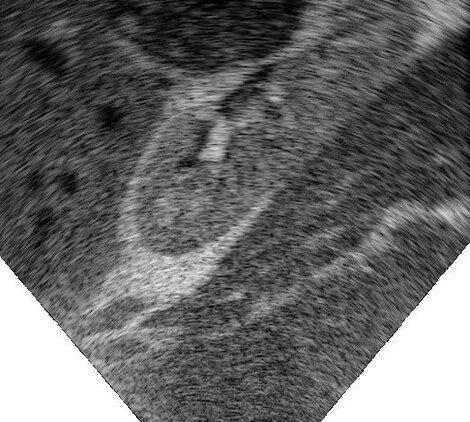
\includegraphics[width=0.33\textwidth]{img/speck ultrasuoni.jpg}
    \hspace{2em}
    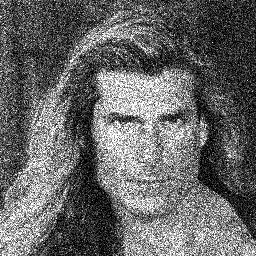
\includegraphics[width=0.33\textwidth]{img/puason.jpg}
\end{frame}

% Slide 4: Tipi di rumore
\begin{frame}{Tipologie di rumore}
    \begin{itemize}
        \item Rumore Gaussiano: disturbi elettronici
        \item Rumore Poissoniano: statistica dei fotoni
        \item Rumore Salt-and-Pepper: errori di trasmissione
        \item Rumore reale da sensori (es. smartphone)
        \item Rumore speckle (ultrasuoni)
    \end{itemize}
    \vspace{0.5cm}
    \begin{center}
        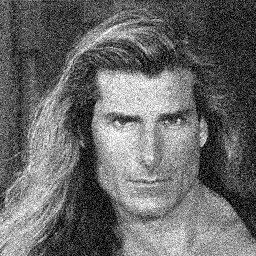
\includegraphics[width=0.2\linewidth]{img/awgn.jpg}
        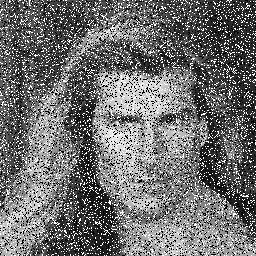
\includegraphics[width=0.2\linewidth]{img/s&p.jpg}
        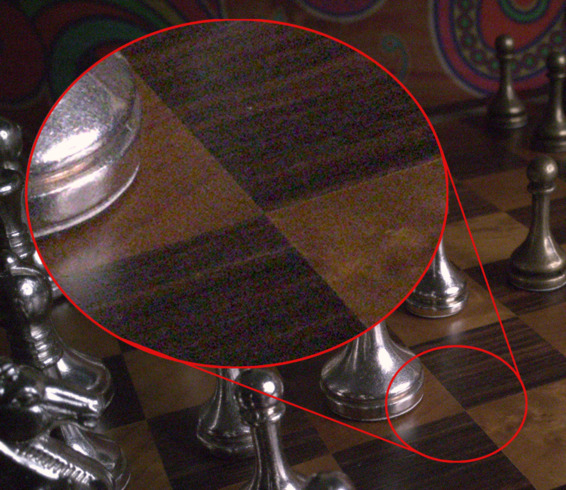
\includegraphics[width=0.2\linewidth]{img/img_dataset/ssid/scacchi_noise_zoom.jpg}
        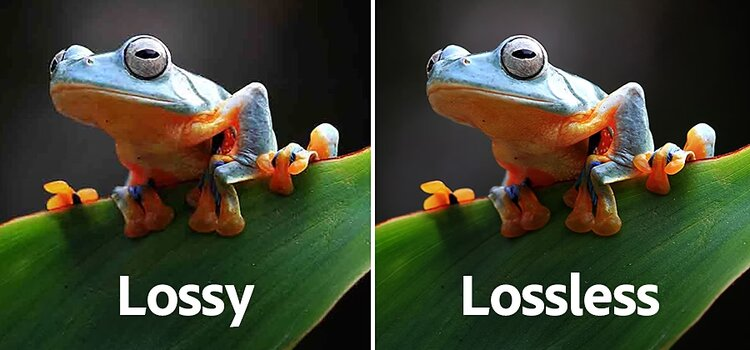
\includegraphics[width=0.3\linewidth]{img/frog.jpg}
    \end{center}
\end{frame}


% Slide 5: Metodi tradizionali
\begin{frame}{Metodi tradizionali}
  \begin{columns}{T}
    \begin{column}{0.4\textwidth}
      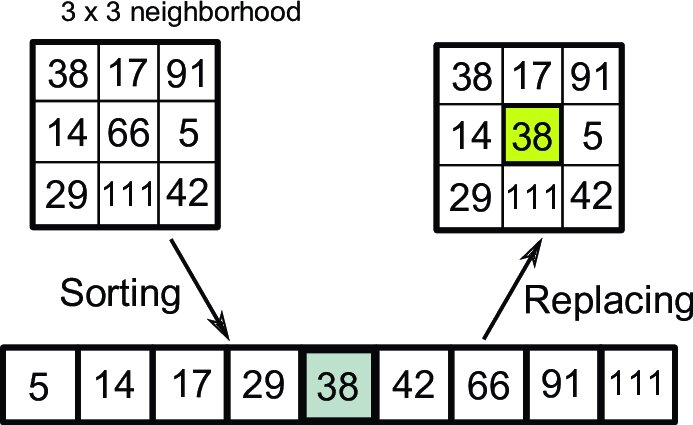
\includegraphics[width=0.7\linewidth]{img/median_filter.jpg}
      \vspace{1.5em}
      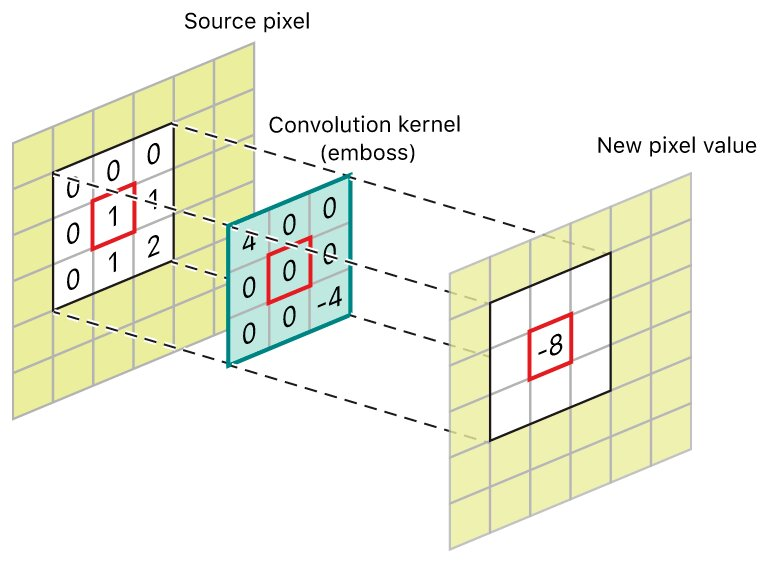
\includegraphics[width=0.7\linewidth]{img/gaussian_filter.jpg}
      \vspace{1.5em}
      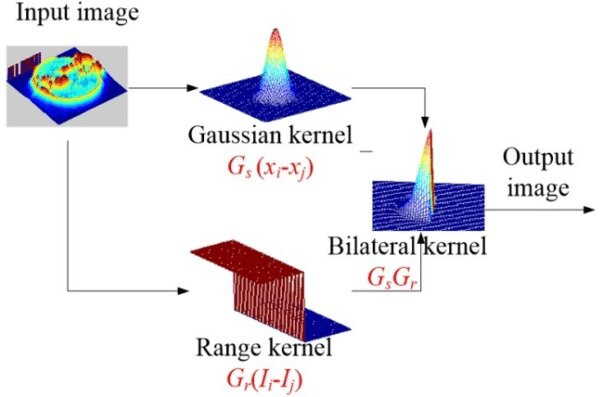
\includegraphics[width=0.7\linewidth]{img/bilateral filter.jpg}
    \end{column}

    \begin{column}{0.55\textwidth}
      \begin{itemize}
        \item Filtri mediani e gaussiani
        \item Non-Local Means
        \item BM3D
      \end{itemize}
    \end{column}
  \end{columns}
\end{frame}


% Un architettura per pagina con qualche dettaglio sui blocchi principali
% Slide 6: Metodi deep learning
\begin{frame}{Metodi deep learning}
    \begin{itemize}
        \item Reti neurali convoluzionali (CNN)
        \item Approcci auto-supervisionati (Noise2Noise) e non supervisionati
        \item Reti generative avversarie (GAN)
    \end{itemize}
\end{frame}

% Slide 7: Le tre reti utilizzate
\begin{frame}{Architetture considerate - 1}
\textbf{RIDNet (Residual Image Denoising Network)} \\
\begin{itemize}
    \item Architettura modulare: estrazione feature, apprendimento residuo, ricostruzione immagine
    \item Normalizzazione iniziale (MeanShift), convoluzioni base, 4 blocchi principali (Merge Run Dual, ResidualBlock, EResidualBlock, CALayer)
    \item Convoluzioni 3x3, 64 feature map, output con 3 filtri e padding "same"
    \item Residual learning: somma residua con input e normalizzazione inversa
    \item Loss: errore quadratico medio (MSE) tra immagine denoisata e pulita
\end{itemize}
\includegraphics[width=\textwidth]{img/ridnet_arch.png}
\end{frame}

\begin{frame}{Architetture considerate - 2}
\textbf{DnCNN (Denoising Convolutional Neural Network)} \\
\begin{itemize}
    \item Rete convoluzionale profonda per la rimozione del rumore tramite apprendimento del residuo
    \item 20 strati convoluzionali: primo con ReLU, 17 con batch normalization + ReLU, ultimo per stima rumore
    \item Tutti i layer convoluzionali: filtri 3x3, 64 feature map; ultimo layer con 3 filtri senza attivazione
    \item Residual learning: sottrazione della stima del rumore dall’immagine originale
    \item Loss: errore quadratico medio (MSE) tra immagine pulita e ricostruita
\end{itemize}
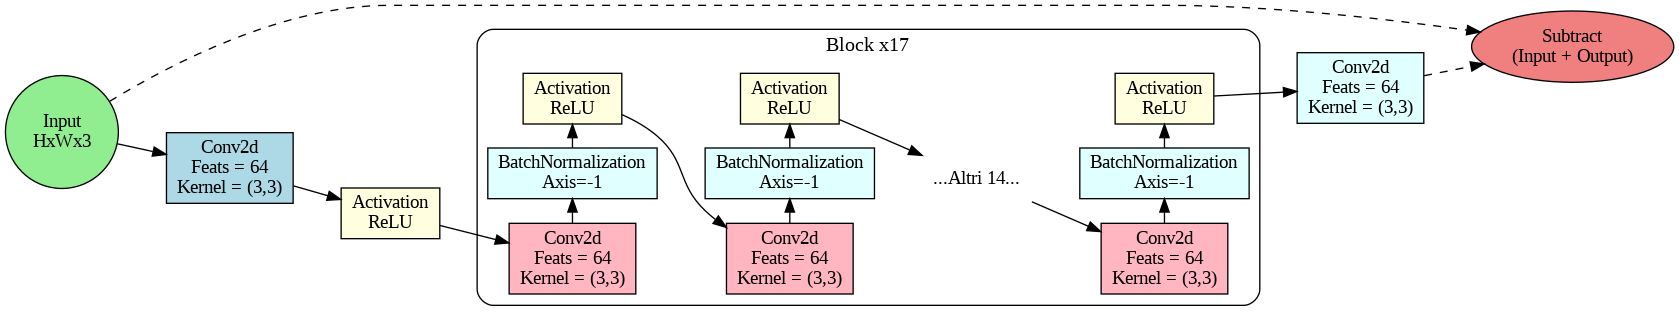
\includegraphics[width=\textwidth]{img/dncnn_arch.png}
\end{frame}

\begin{frame}{Architetture considerate - 3}
\textbf{Autoencoder} \\

\begin{itemize}
    \item Architettura generica per apprendere rappresentazioni compatte dai dati
    \item Composta da encoder (compressione) e decoder (ricostruzione)
    \item Compressione elimina il rumore, decoder ricostruisce le strutture coerenti
    \item Implementato con 5 strati convoluzionali, MaxPooling, UpSampling, filtri 3x3, 64 feature map, ultimo layer con 3 filtri
    \item Loss: errore quadratico medio (MSE) tra immagine ricostruita e pulita
\end{itemize}

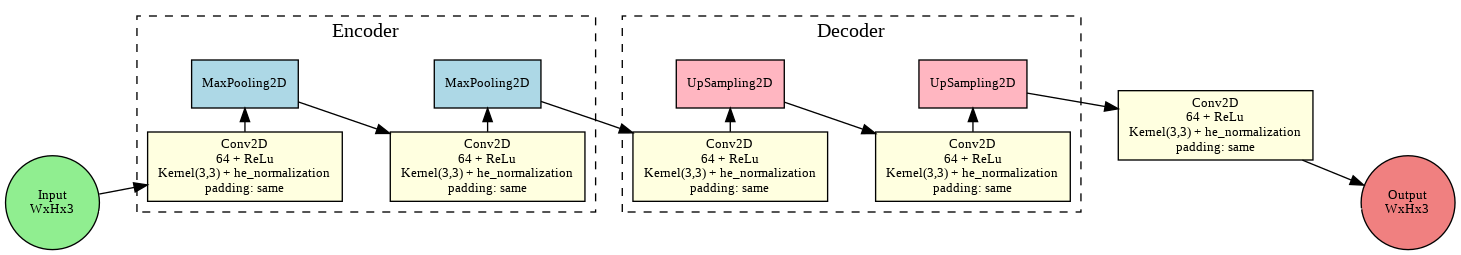
\includegraphics[width=\textwidth]{img/autoen_arch.png}
\end{frame}



% dividere uno per slide con immgini di esempio
% Slide 8: Dataset utilizzati

% Slide: SIDD
\begin{frame}{Dataset utilizzati - SIDD}
    \begin{itemize}
        \item Il \textbf{Smartphone Image Denoising Dataset} contiene immagini acquisite da smartphone in condizioni reali, con rumore autentico dovuto a scarsa luminosità e vari livelli ISO.
        \item Ogni immagine noisy è accompagnata dalla versione clean, ottenuta tramite esposizioni multiple.
        \item Utilizzato per valutare la robustezza dei modelli su rumore reale.
    \end{itemize}
    \centering
    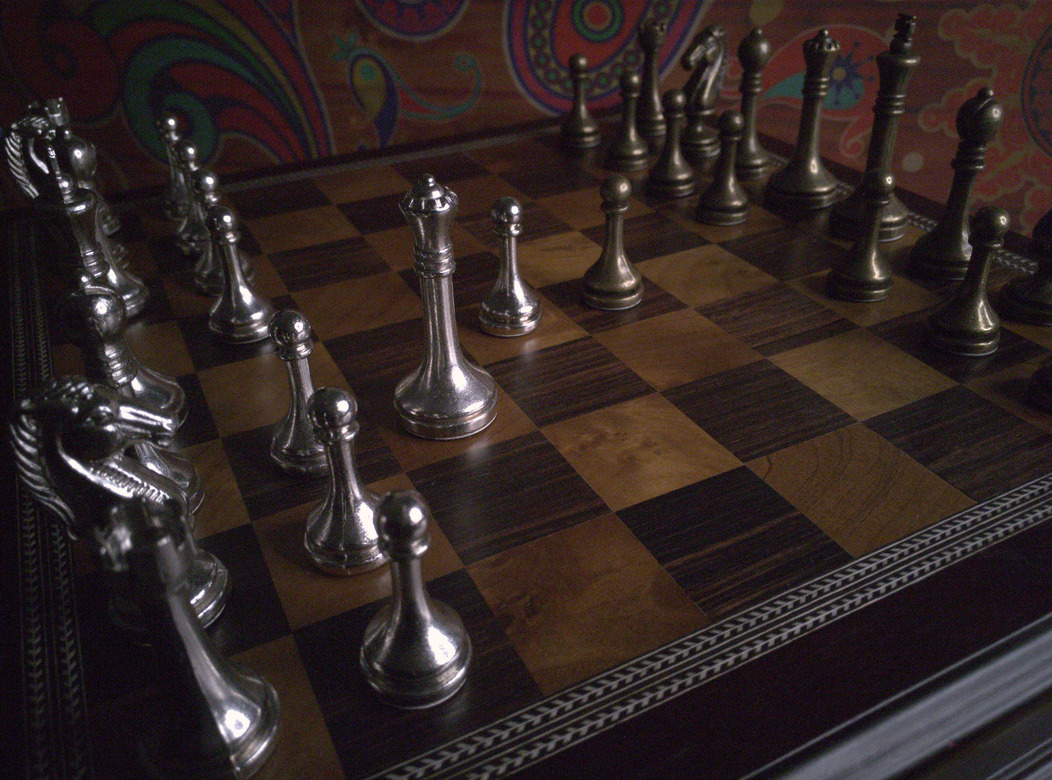
\includegraphics[height=0.22\textheight]{img/img_dataset/ssid/scacchi_noisy.jpg}
    \hspace{1.5em}
    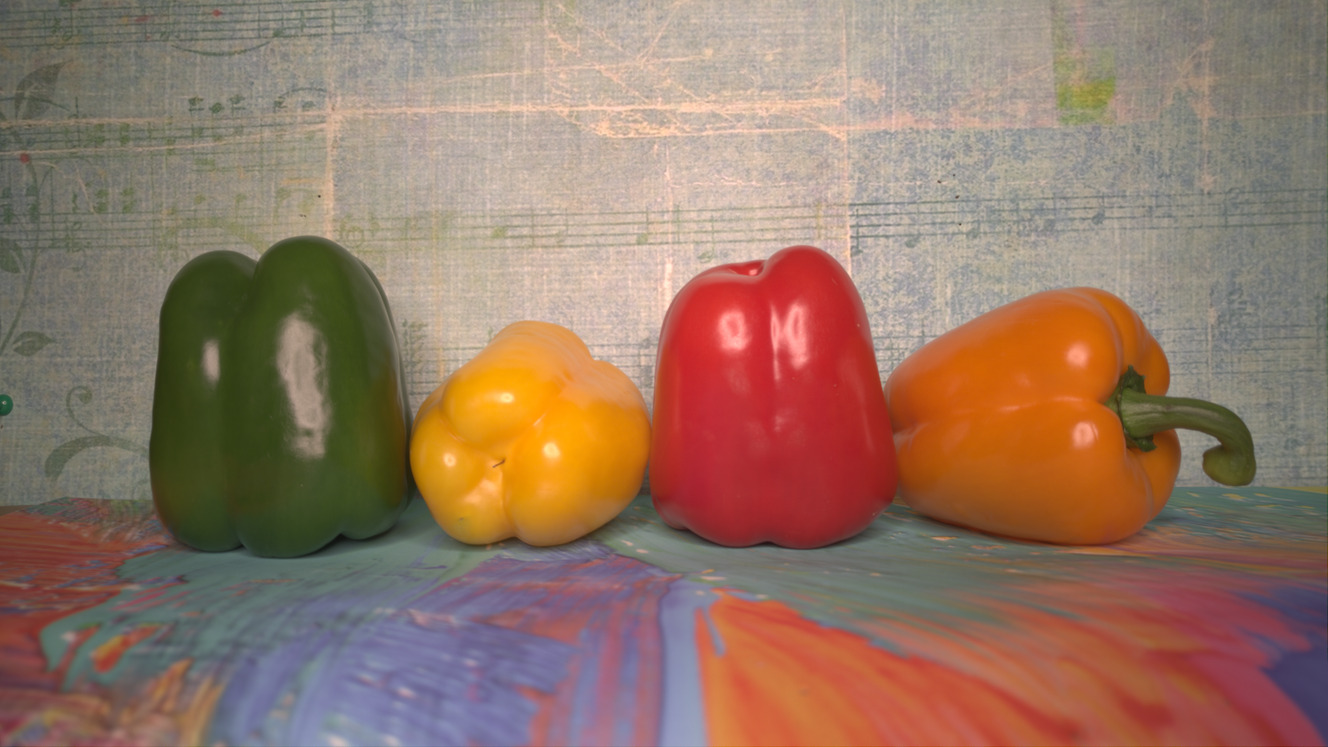
\includegraphics[height=0.22\textheight]{img/img_dataset/ssid/peperoni.jpg}
    \hspace{1.5em}
    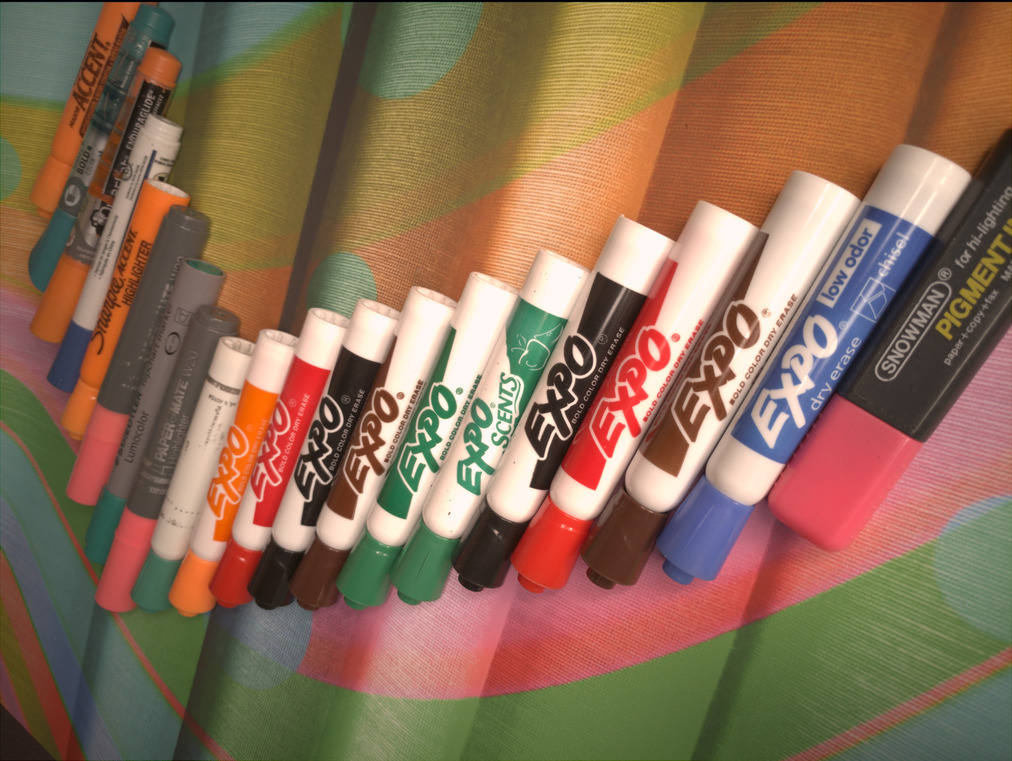
\includegraphics[height=0.22\textheight]{img/img_dataset/ssid/colori.jpg}
\end{frame}

% Slide: Renoir
\begin{frame}{Dataset utilizzati - Renoir}
    \begin{itemize}
        \item Il dataset \textbf{Renoir} raccoglie immagini reali scattate in condizioni di luce variabile, con diversi livelli di esposizione e rumore.
        \item Permette di testare i modelli su scene indoor e outdoor, con rumore non sintetico.
        \item Include versioni noisy e clean per ogni scena.
    \end{itemize}
    \centering
    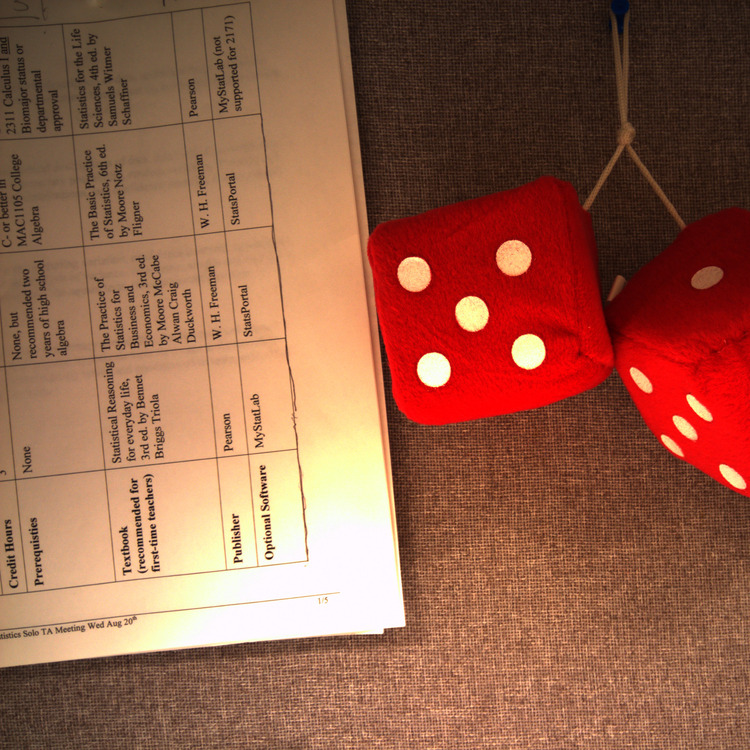
\includegraphics[height=0.22\textheight]{img/img_dataset/renoir/mi3_dadi.jpg}
    \hspace{1.5em}
    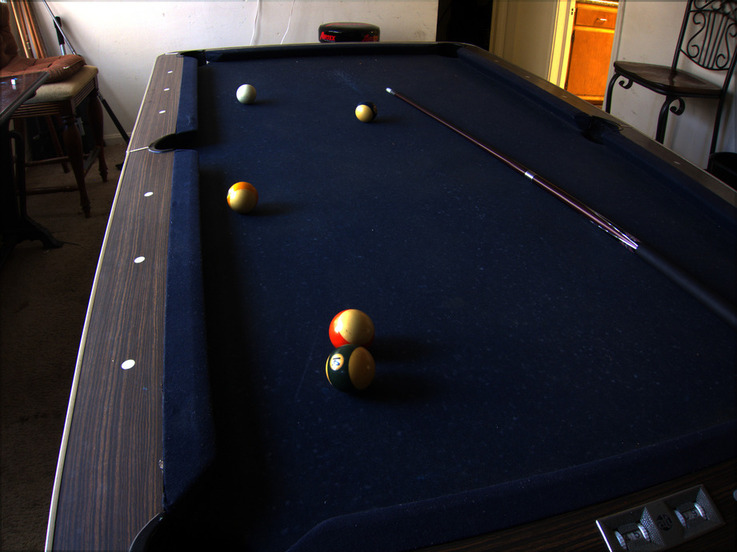
\includegraphics[height=0.22\textheight]{img/img_dataset/renoir/s90_biliardo.jpg}
    \hspace{1.5em}
    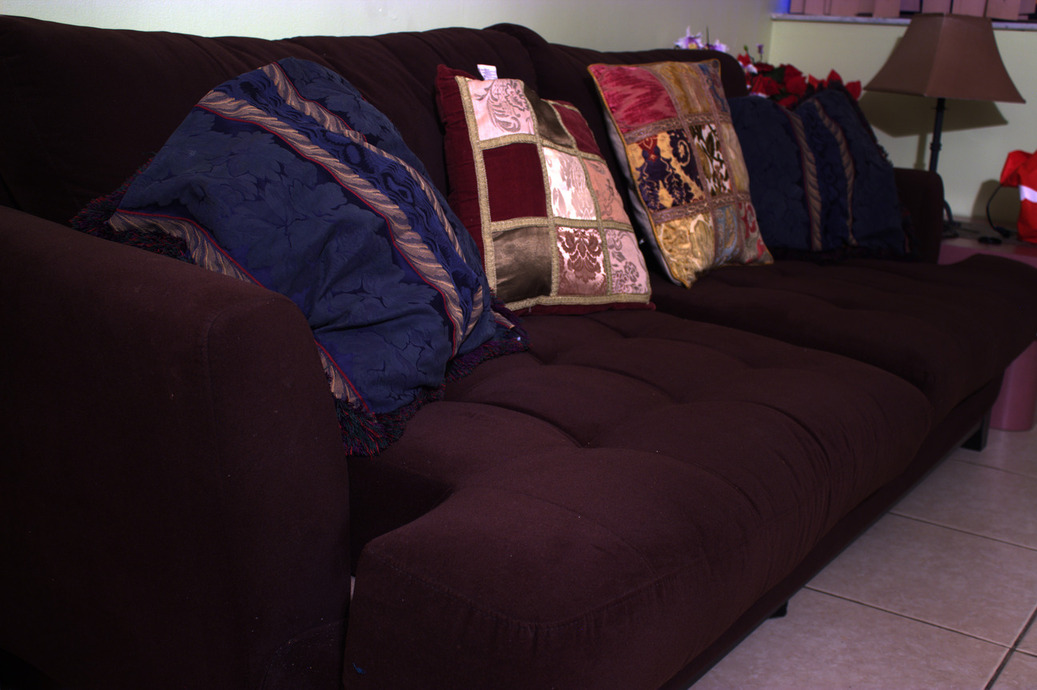
\includegraphics[height=0.22\textheight]{img/img_dataset/renoir/t3i_divano.jpg}
\end{frame}

% Slide: BSD500
\begin{frame}{Dataset utilizzati - BSD500}
    \begin{itemize}
        \item Il \textbf{Berkeley Segmentation Dataset} è composto da immagini naturali di vario tipo, spesso usato come benchmark per algoritmi di visione.
        \item Su queste immagini viene aggiunto rumore sintetico di diversi livelli per testare la capacità di denoising.
        \item Ampia varietà di soggetti e scene.
    \end{itemize}
    \centering
    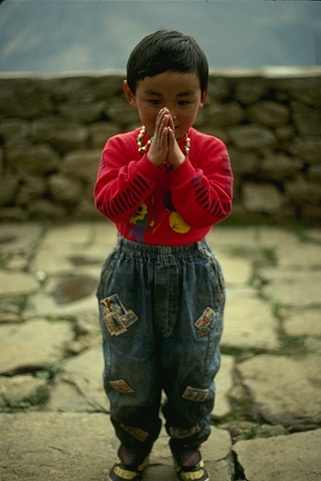
\includegraphics[height=0.22\textheight]{img/img_dataset/bsd/bimba.jpg}
    \hspace{1.5em}
    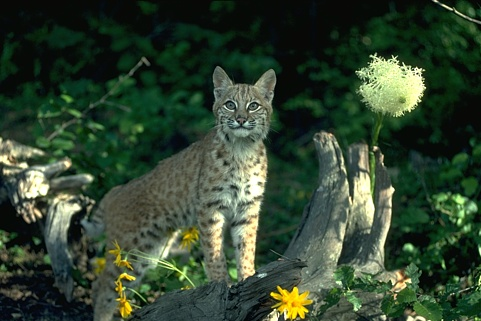
\includegraphics[height=0.22\textheight]{img/img_dataset/bsd/gattp.jpg}
    \hspace{1.5em}
    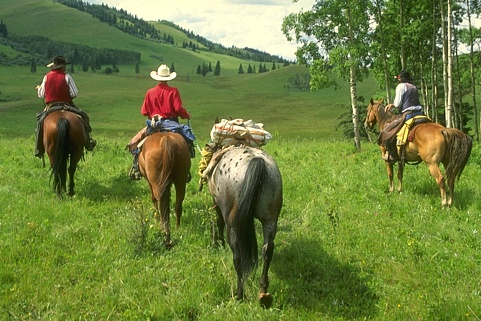
\includegraphics[height=0.22\textheight]{img/img_dataset/bsd/paesaggio_completo.jpg}
\end{frame}

% Slide: FiveK
\begin{frame}{Dataset utilizzati - FiveK}
    \begin{itemize}
        \item Il \textbf{MIT-Adobe FiveK} contiene immagini fotografiche ad alta qualità, spesso usate per testare algoritmi di miglioramento e denoising.
        \item Le immagini sono di vario genere e vengono degradate con rumore sintetico per la valutazione dei modelli.
        \item Ottimo per test su fotografie professionali.
    \end{itemize}
    \centering
    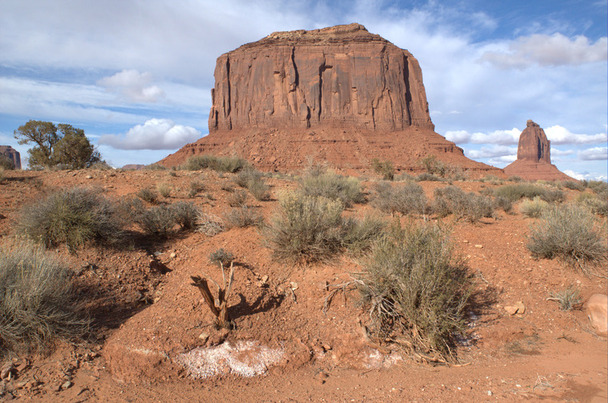
\includegraphics[height=0.22\textheight]{img/img_dataset/fivek/hq1.jpg}
    \hspace{1.5em}
    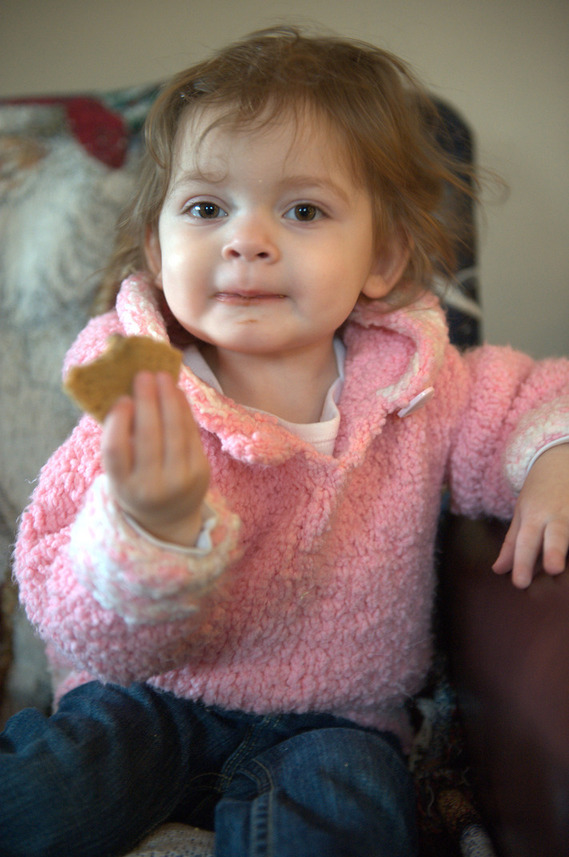
\includegraphics[height=0.22\textheight]{img/img_dataset/fivek/hq2.jpg}
    \hspace{1.5em}
    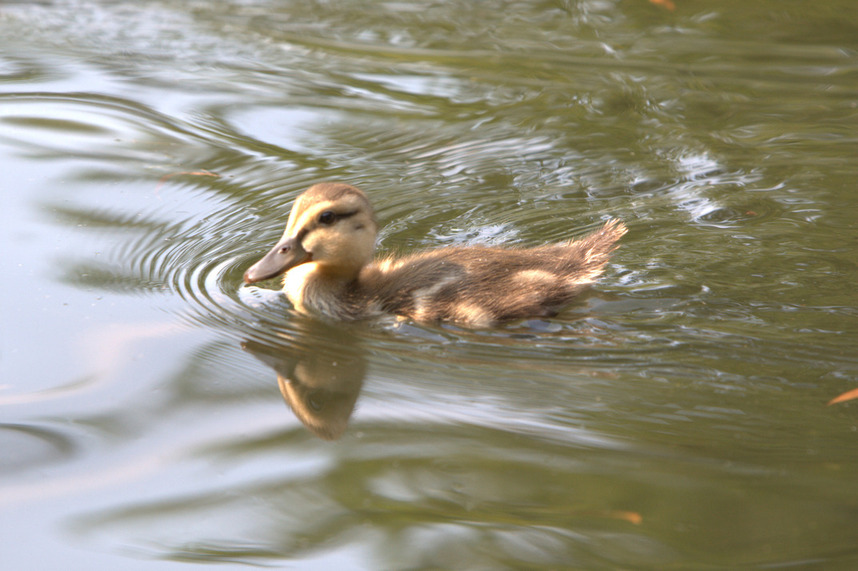
\includegraphics[height=0.22\textheight]{img/img_dataset/fivek/hq6.jpg}
\end{frame}

% Slide: DIV2K
\begin{frame}{Dataset utilizzati - DIV2K}
    \begin{itemize}
        \item Il \textbf{DIV2K} è un dataset di immagini ad alta risoluzione (2K), molto utilizzato per super-risoluzione e denoising.
        \item Le immagini coprono una grande varietà di soggetti e vengono degradate con diversi livelli di rumore.
        \item Utile per valutare le prestazioni su immagini di grandi dimensioni.
    \end{itemize}
    \centering
    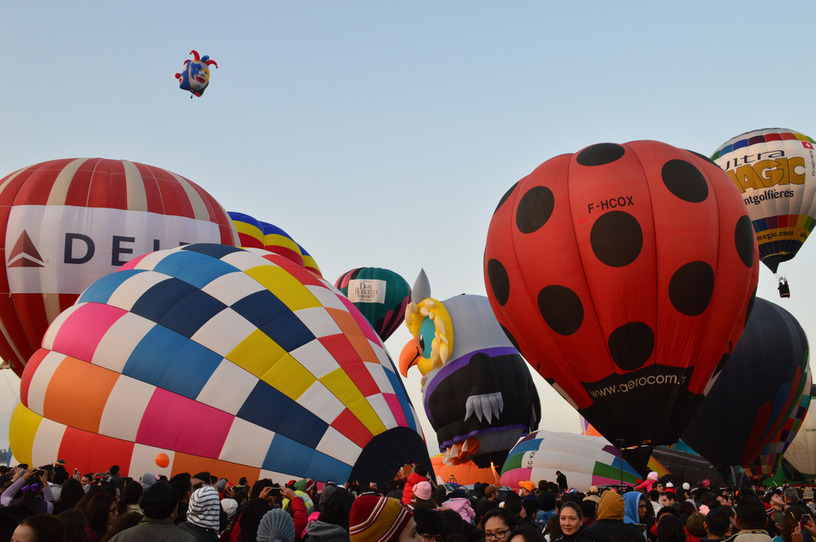
\includegraphics[height=0.22\textheight]{img/img_dataset/div2k/mongolfiere.jpg}
    \hspace{1.5em}
    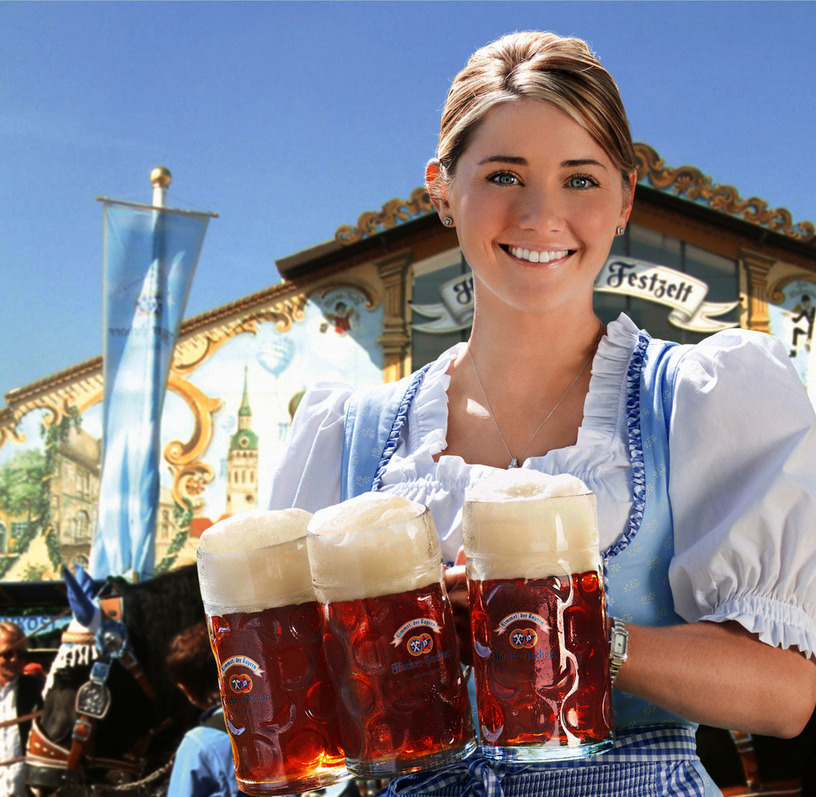
\includegraphics[height=0.22\textheight]{img/img_dataset/div2k/oktoberfest.jpg}
    \hspace{1.5em}
    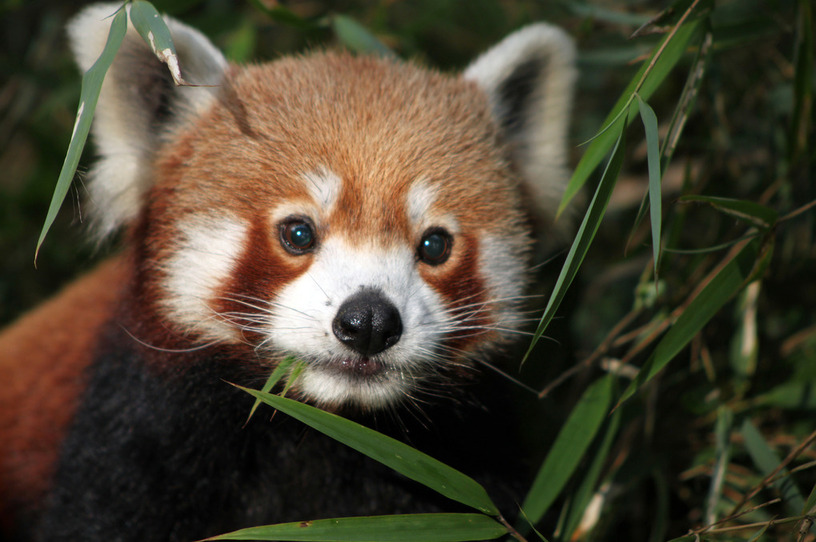
\includegraphics[height=0.22\textheight]{img/img_dataset/div2k/pandar.jpg}
\end{frame}

% Slide: Kvasir
\begin{frame}{Dataset utilizzati - Kvasir}
    \begin{itemize}
        \item \textbf{Kvasir} è un dataset di immagini endoscopiche, utilizzato per testare la capacità di adattamento dei modelli su dati medici.
        \item Le immagini presentano rumore e artefatti tipici delle acquisizioni cliniche.
        \item Fondamentale per valutare il fine tuning e la generalizzazione su domini specifici.
    \end{itemize}
    \centering
    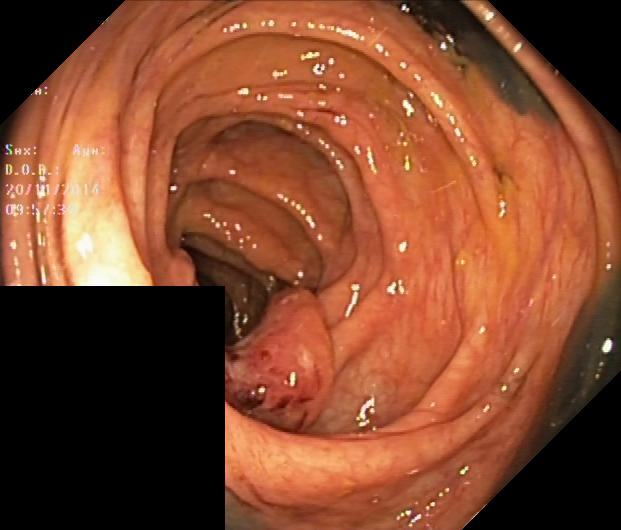
\includegraphics[height=0.22\textheight]{img/img_dataset/kvasir/kvasir_1.jpg}
 \hspace{1.5em}
    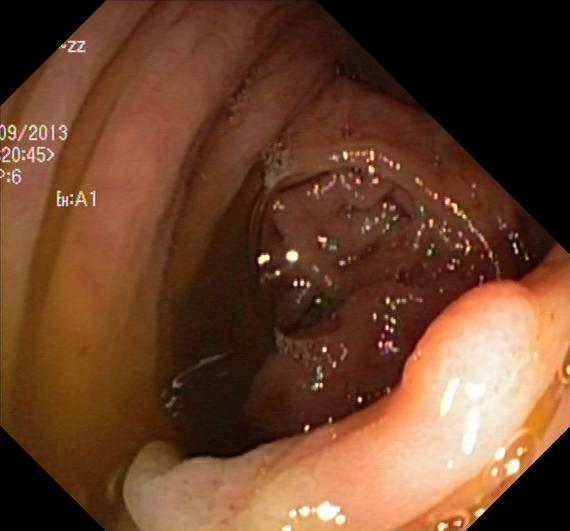
\includegraphics[height=0.22\textheight]{img/img_dataset/kvasir/kvasir_2.jpg}
\hspace{1.5em}
    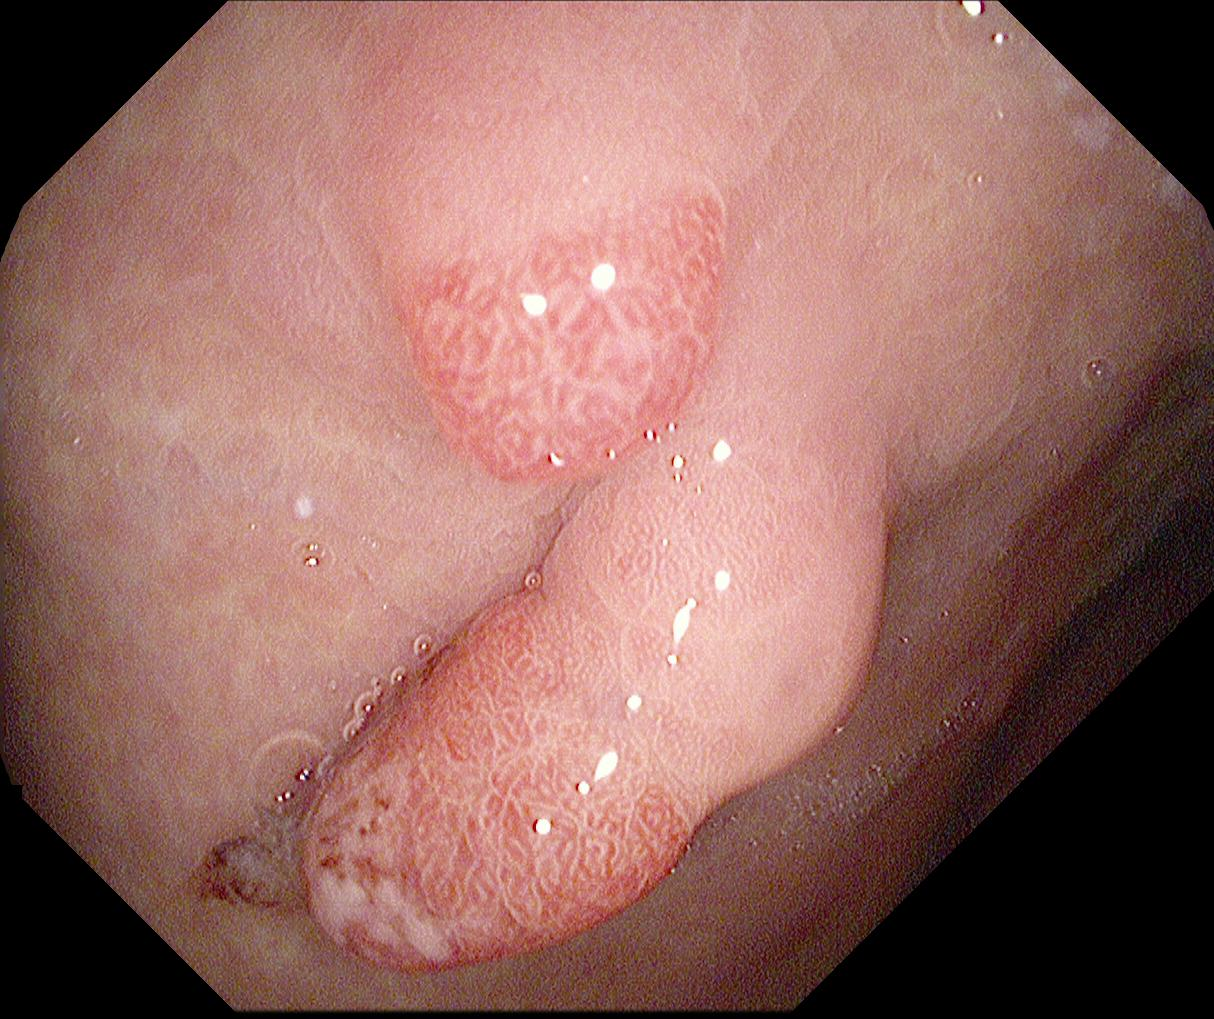
\includegraphics[height=0.22\textheight]{img/img_dataset/kvasir/kvasir_3.jpg}
\end{frame}


% Slide 9: Valutazione dei risultati
\begin{frame}{Metodologia di valutazione}
    \begin{itemize}
        \item Calcolato il PSNR per ogni modello e dataset % forma del psnr
        \item Confronto tra modelli sui diversi dataset e livelli di rumore
        \item Analisi quantitativa e qualitativa
        \item BM3D metodo consolidato, considerato come baseline per il denoising, ti tipo non-learned
    \end{itemize}
\end{frame}

% dettagli sulla sistemazione dei dataset
\begin{frame}{Preprocessing dei dataset di training}
  \begin{itemize}
    \item Dataset usati per il train: SIDD, Renoir, Div2K, BSD500 e FiveK
    \item BSD500 applicato un padding per portare le immagini ad una risoluzione di (512x512)
    \item Gli altri hanno subito un patching di 12 immagini di risoluzione sempre (512x512)
    \item A DIV2K, BSD e FiveK è stato applicato un rumore artficiale casuale tra $\sigma=15,25,50$
    \item Tutti i dataset sono stati mischiati, uniti, rimischiati e suddivisi al 60\% per il training e 20\% per validation e accuracy
  \end{itemize}
\end{frame}


\begin{frame}{Preprocessing: Padding}
    \centering
    \begin{tikzpicture}
        % Riduci la distanza tra le immagini per evitare overflow
        \node[anchor=east] (A) at (0,0) {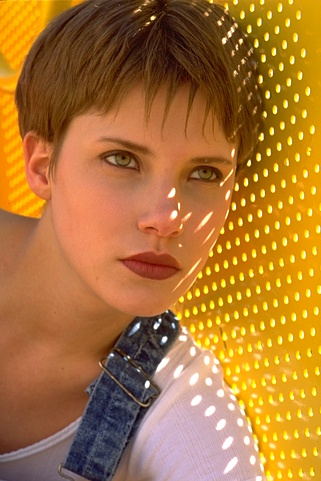
\includegraphics[width=0.38\linewidth]{img/img_dataset/bsd/signorina.jpg}};
        \node[anchor=west] (B) at (2,0) {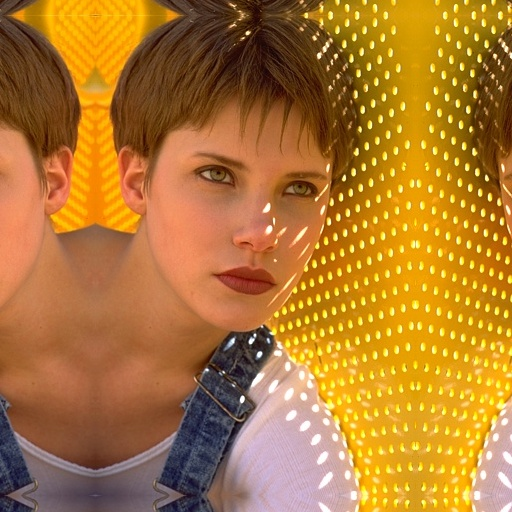
\includegraphics[width=0.38\linewidth]{img/img_dataset/bsd/signorina specchiata.jpg}};
        \draw[thick,->] (A.east) -- (B.west);
    \end{tikzpicture}
\end{frame}

\begin{frame}{Preprocessing: Patching}
    \centering
    \begin{tikzpicture}
        % Immagine originale a sinistra
        \node[anchor=east] (A) at (0,0) {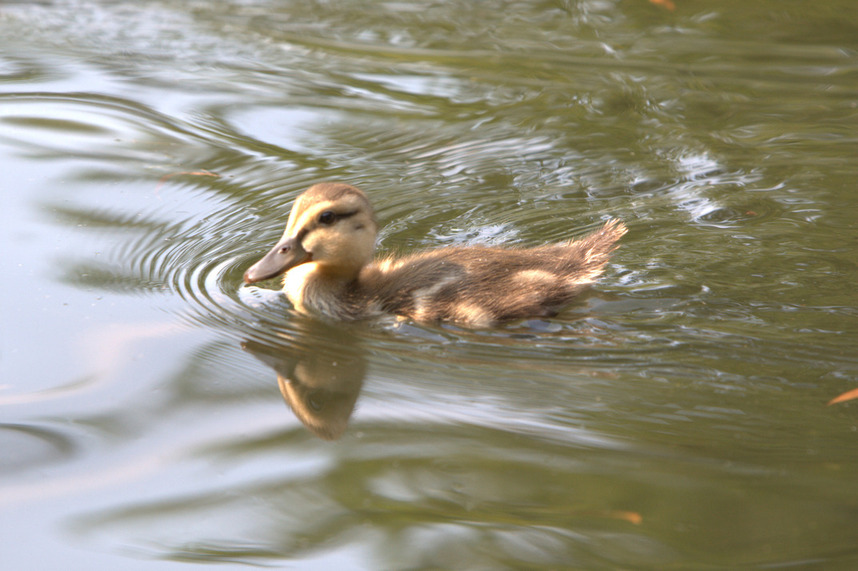
\includegraphics[width=0.4\linewidth]{img/img_dataset/fivek/hq6.jpg}};
        % Tabella delle patch a destra
        \node[anchor=west] (B) at (1,0) {
            \begin{tabular}{cccc}
                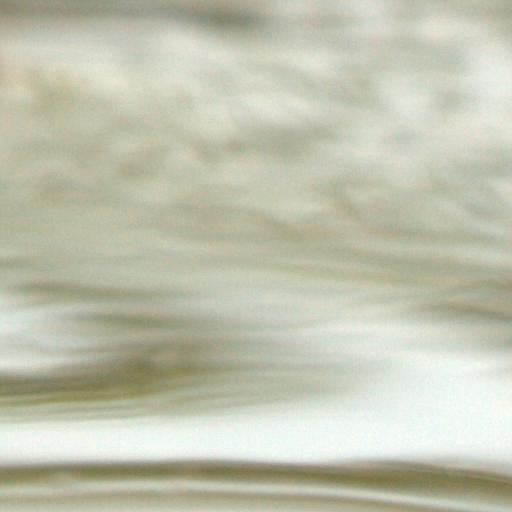
\includegraphics[width=0.09\linewidth]{img/img_dataset/fivek/patch/hq6_patch0.jpg} &
                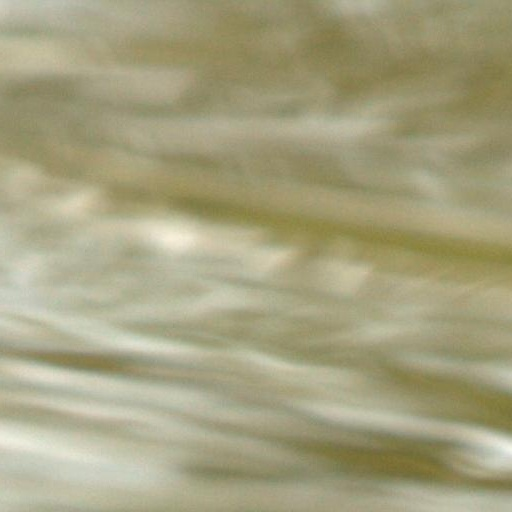
\includegraphics[width=0.09\linewidth]{img/img_dataset/fivek/patch/hq6_patch1.jpg} &
                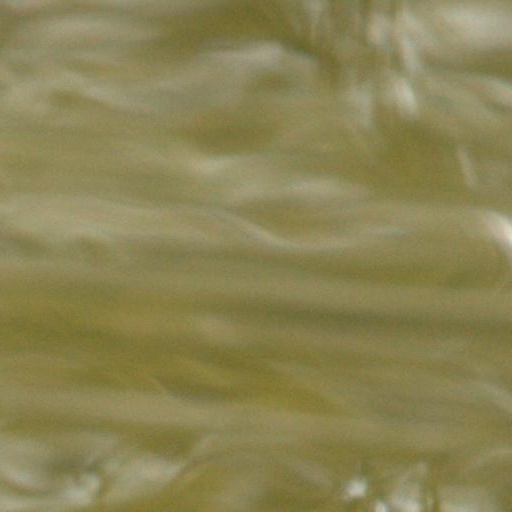
\includegraphics[width=0.09\linewidth]{img/img_dataset/fivek/patch/hq6_patch2.jpg} &
                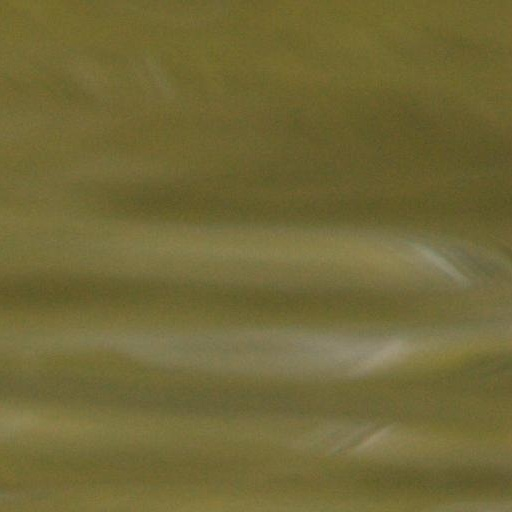
\includegraphics[width=0.09\linewidth]{img/img_dataset/fivek/patch/hq6_patch3.jpg} \\
                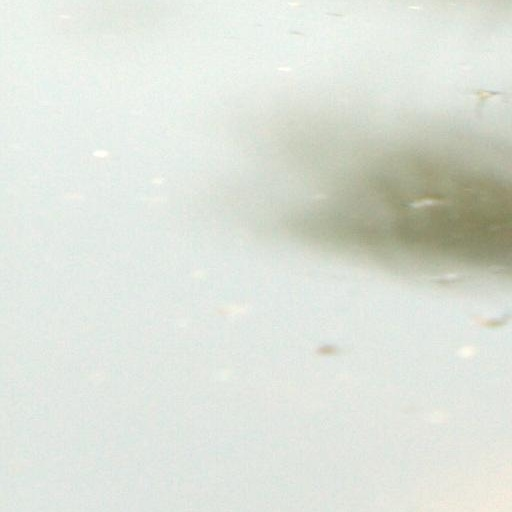
\includegraphics[width=0.09\linewidth]{img/img_dataset/fivek/patch/hq6_patch4.jpg} &
                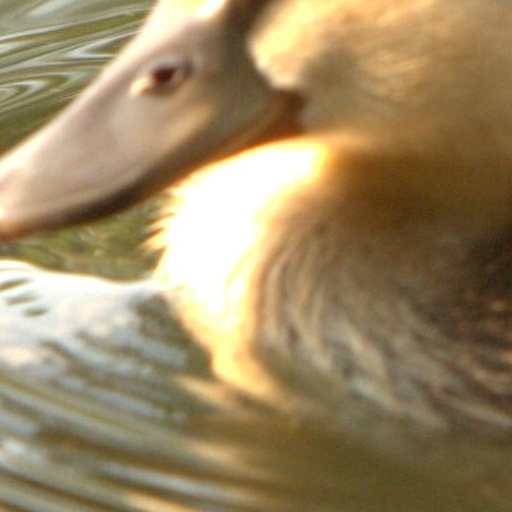
\includegraphics[width=0.09\linewidth]{img/img_dataset/fivek/patch/hq6_patch5.jpg} &
                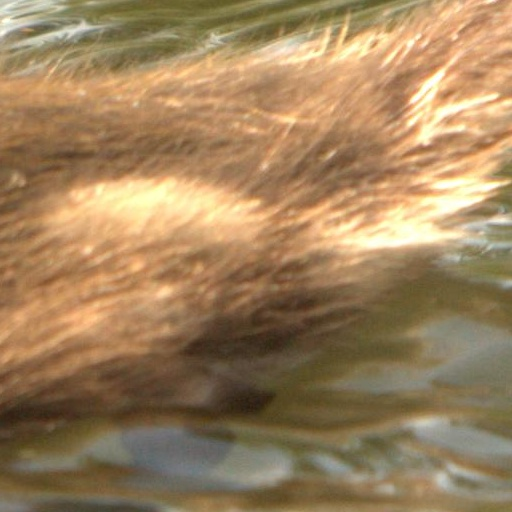
\includegraphics[width=0.09\linewidth]{img/img_dataset/fivek/patch/hq6_patch6.jpg} &
                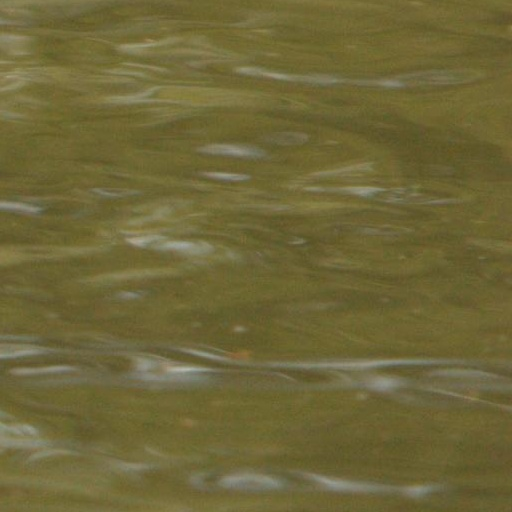
\includegraphics[width=0.09\linewidth]{img/img_dataset/fivek/patch/hq6_patch7.jpg} \\
                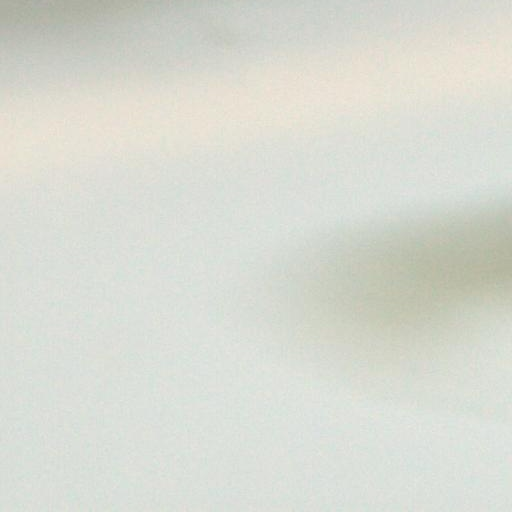
\includegraphics[width=0.09\linewidth]{img/img_dataset/fivek/patch/hq6_patch8.jpg} &
                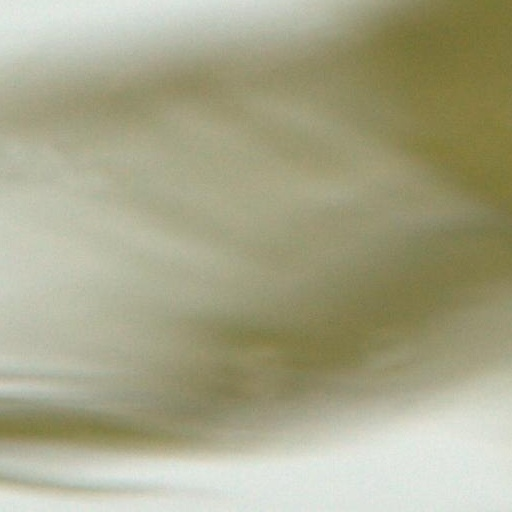
\includegraphics[width=0.09\linewidth]{img/img_dataset/fivek/patch/hq6_patch9.jpg} &
                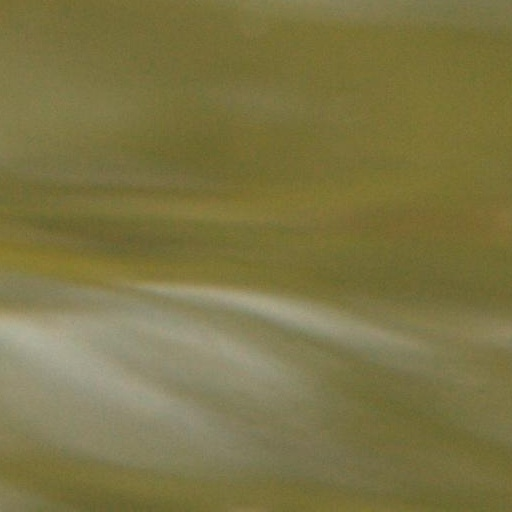
\includegraphics[width=0.09\linewidth]{img/img_dataset/fivek/patch/hq6_patch10.jpg} &
                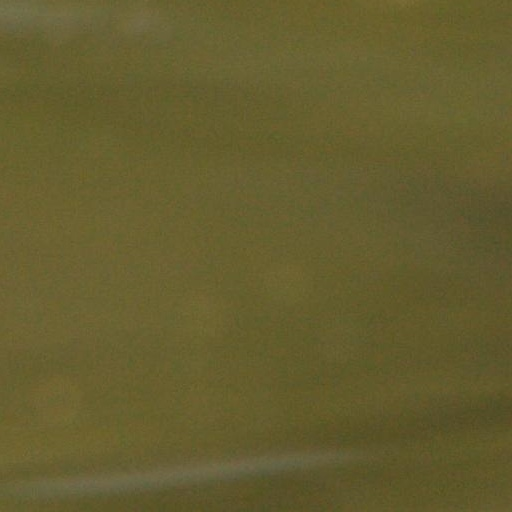
\includegraphics[width=0.09\linewidth]{img/img_dataset/fivek/patch/hq6_patch11.jpg} \\
            \end{tabular}
        };
        % Freccia dalla foto originale alla tabella delle patch
        \draw[thick,->] (A.east) -- (B.west);
    \end{tikzpicture}
\end{frame}

\begin{frame}{Preprocessing: Rumore}
    \centering
    \begin{tikzpicture}
        % Nodo immagine originale
        \node (orig) at (0,0) {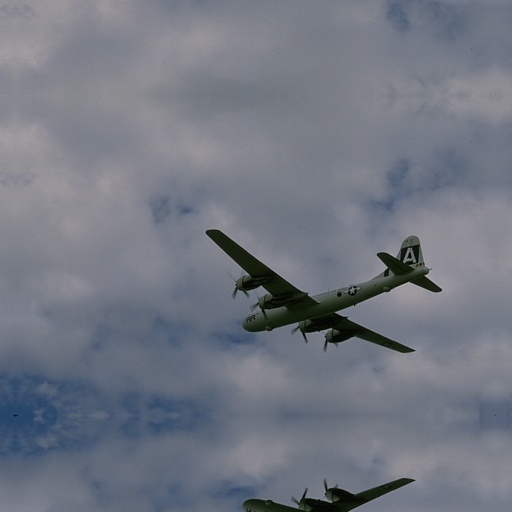
\includegraphics[width=0.25\linewidth]{img/noise/aereo.jpg}};
        % Nodi immagini noisy, posizionati più distanti
        \node (n15) at (-4,-4) {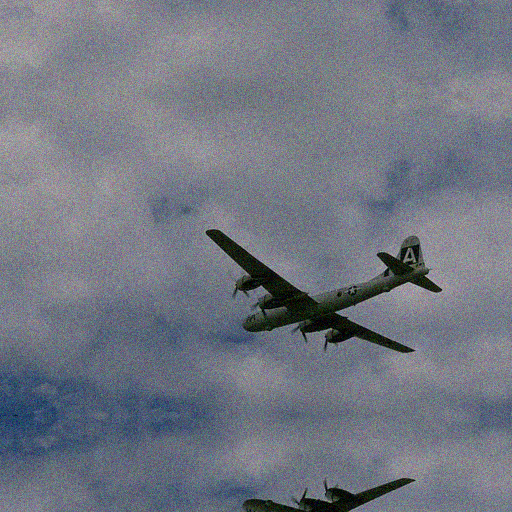
\includegraphics[width=0.22\linewidth]{img/noise/noisy_aereo_15.png}};
        \node (n25) at (0,-4.5) {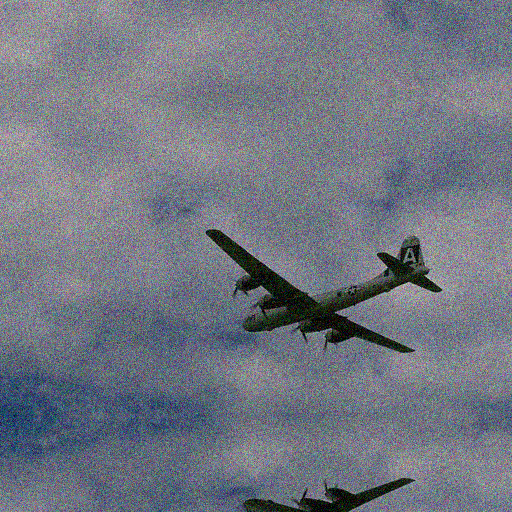
\includegraphics[width=0.22\linewidth]{img/noise/noisy_aereo_25.png}};
        \node (n50) at (4,-4) {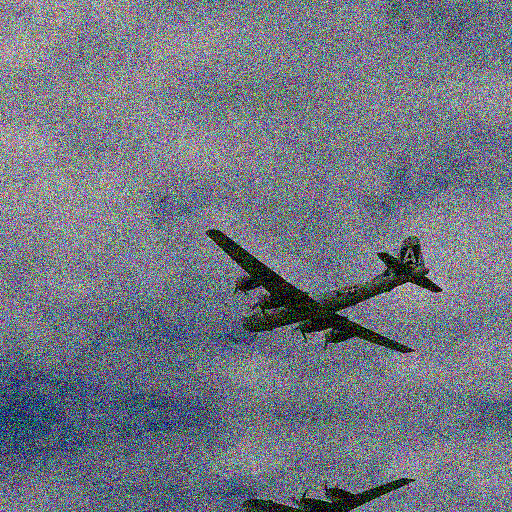
\includegraphics[width=0.22\linewidth]{img/noise/noisy_aereo_50.png}};
        % Frecce con etichette
        \draw[thick,->] (orig.south west) -- node[left, font=\small] {$\sigma=15$} (n15.north);
        \draw[thick,->] (orig.south) -- node[right, font=\small] {$\sigma=25$} (n25.north);
        \draw[thick,->] (orig.south east) -- node[right, font=\small] {$\sigma=50$} (n50.north);
    \end{tikzpicture}
\end{frame}

% Varie slide con i grafici del trainig, dimensioni dei sub dataset
% prestazioni con gli iperparametri consigliati
\begin{frame}{Risultati training: RIDNet}

  \begin{itemize}
      \item RIDNet inizializzato con input flessibile (qualsiasi risoluzione, 3 canali RGB).
      \item Iperparametri principali scelti dagli autori: 64 feature map (n\_feats) e reduction 16 nei blocchi di attenzione.
      \item Ottimizzatore Adam con learning rate 1e-4.
      \item Loss: Mean Squared Error (MSE), adatta al denoising.
      \item Accuracy monitorata durante il training.
      \item Setup pensato per denoising su immagini di qualsiasi dimensione.
  \end{itemize}

  \begin{columns}[T]
    \begin{column}{0.5\linewidth}
      \centering
      RIDNet - Training Loss\\
      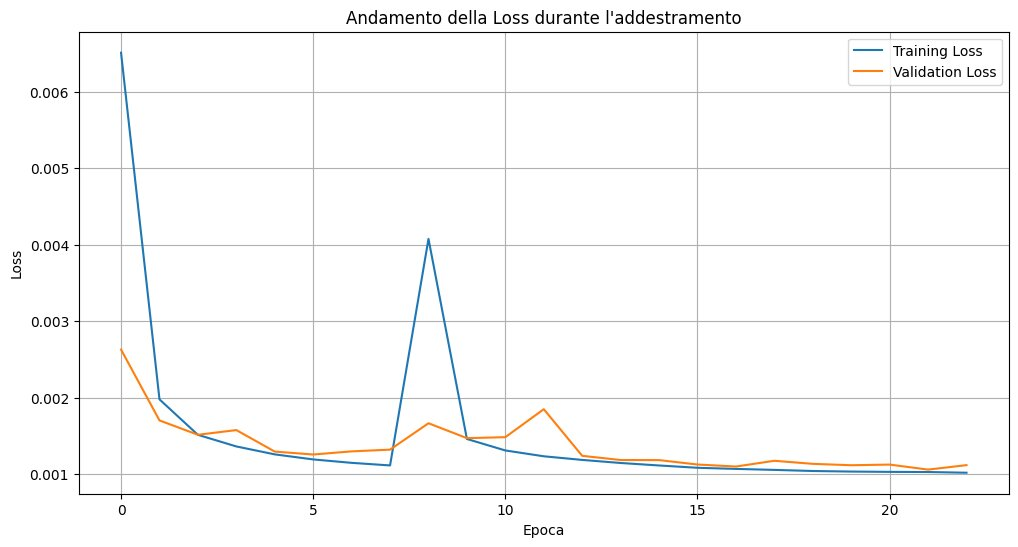
\includegraphics[width=0.8\linewidth]{img/Ridnet_loss.jpg}\\[0.5em]
    \end{column}
    \begin{column}{0.5\linewidth}
      \centering
      RIDNet - Training Accuracy\\
      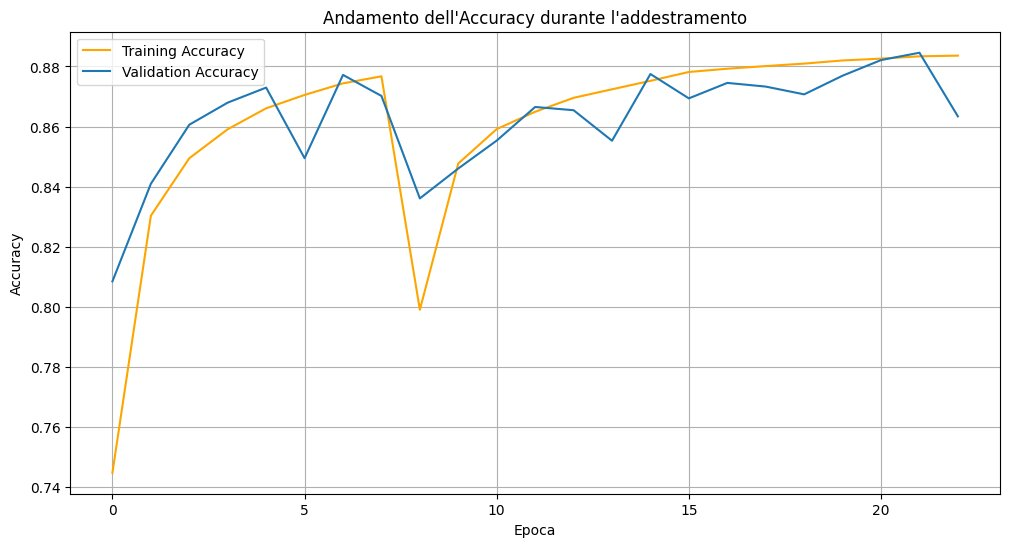
\includegraphics[width=0.8\linewidth]{img/Ridnet_accuracy.jpg}
    \end{column}
  \end{columns}
\end{frame}

% Slide 7: Le tre reti utilizzate
\begin{frame}{Risultati training: DnCNN}

  \begin{itemize}
      \item DnCNN addestrato per apprendere il rumore residuo da sottrarre all'immagine rumorosa.
      \item Batch normalization e ReLU stabilizzano il training.
      \item Modello creato per input di qualsiasi dimensione e 3 canali (RGB).
      \item Ottimizzatore Adam con learning rate 1e-4, loss MSE, metrica accuracy.
      \item Iperparametri: 64 feature e 16 reduction
  \end{itemize}

  \begin{columns}[T]
    \begin{column}{0.5\linewidth}
      \centering
      DnCNN - Training Loss\\
      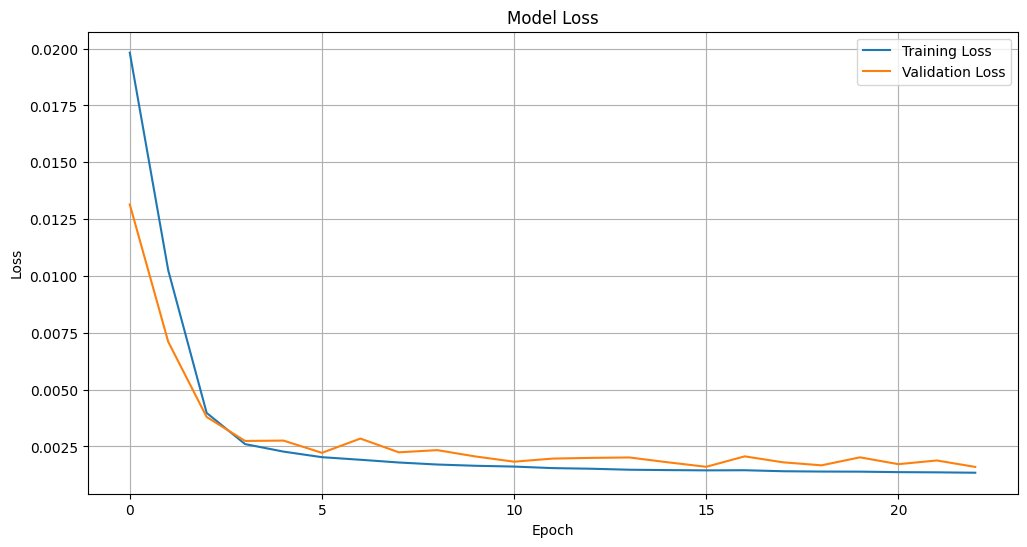
\includegraphics[width=0.8\linewidth]{img/DnCNN_loss.jpg}\\[0.5em]
    \end{column}
    \begin{column}{0.5\linewidth}
      \centering
      DnCNN - Training Accuracy\\
      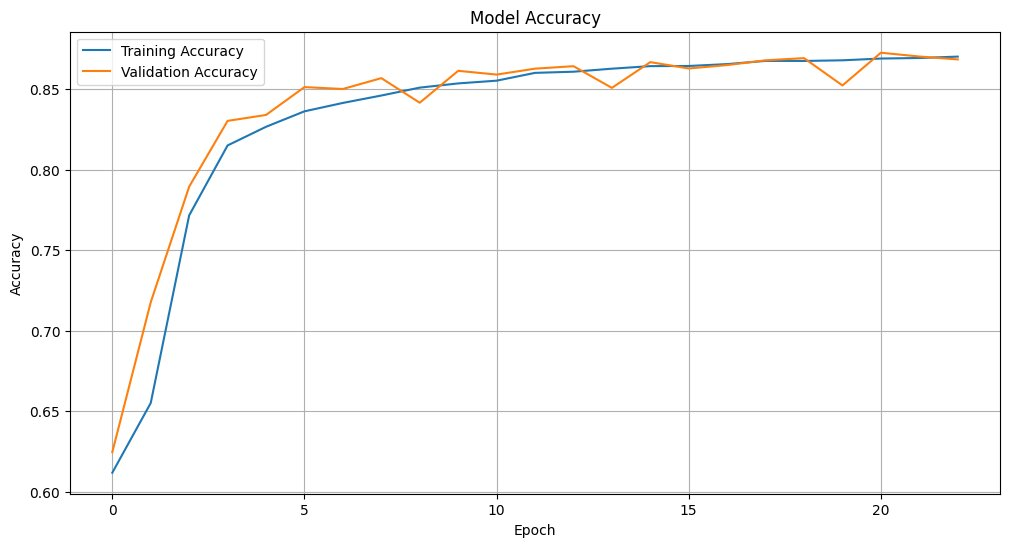
\includegraphics[width=0.8\linewidth]{img/DnCNN_accuracy.jpg}
    \end{column}
  \end{columns}
\end{frame}

\begin{frame}{Risultati training: Autoencoder}

  \begin{itemize}
      \item Autoencoder allenato come architettura compressiva, sfruttando codifica e decodifica per ridurre il rumore.
      \item Creato per input di qualsiasi dimensione e 3 canali (RGB).
      \item Compilato con Adam, loss MSE e accuratezza come metrica.
      \item Iperparametri: 64 fetaure e 16 reduction
  \end{itemize}

  \begin{columns}[T]
    \begin{column}{0.5\linewidth}
      \centering
      Autoencoder - Training Loss\\
      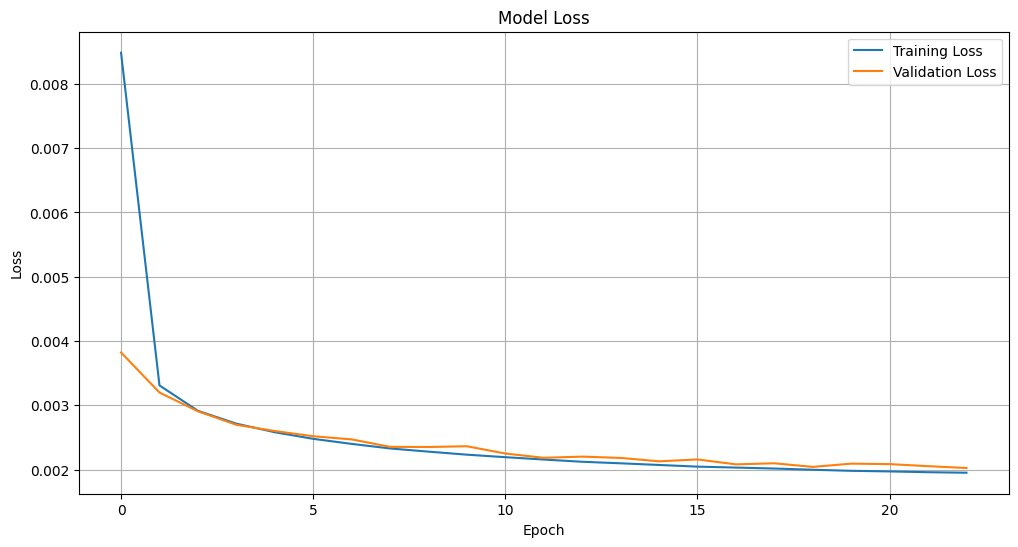
\includegraphics[width=0.9\linewidth]{img/Autoen_loss.jpg}\\[0.5em]
    \end{column}
    \begin{column}{0.5\linewidth}
      \centering
      Autoencoder - Training Accuracy\\
      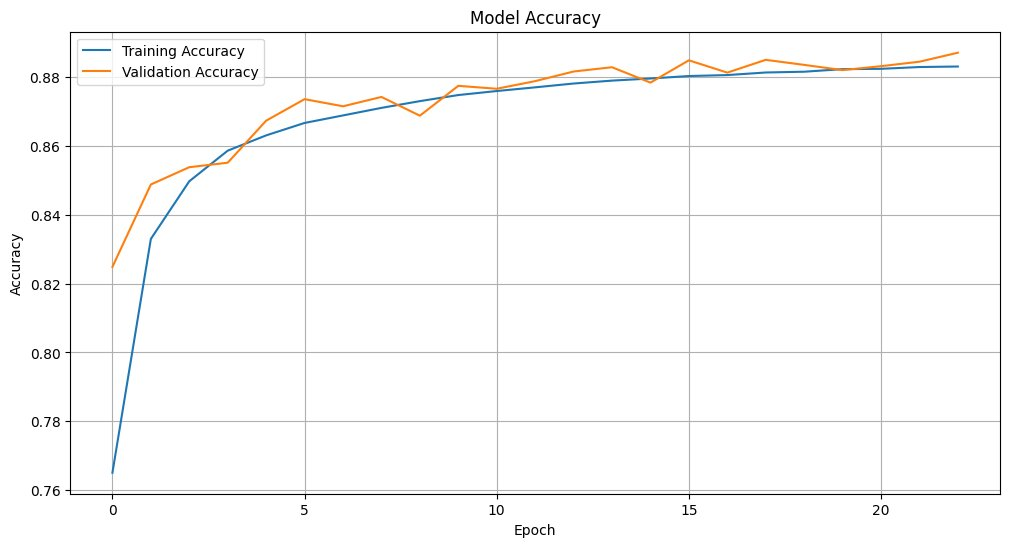
\includegraphics[width=0.9\linewidth]{img/Autoen_accuracy.jpg}
    \end{column}
  \end{columns}
\end{frame}


% RISULTATI TRAINING












%%%%%%%%%%%%%%%%%% TAMBURO  %%%%%%%%%%%%%%%%%%%%%%%%%%%%%%%%%%%%%%%%%%%%%%%%%%%%%%%%%%%%%%%%%%

% --- Tamburo σ=15 ---
\begin{frame}{Denoising: $\sigma=15$ (Tamburo)}
    \centering
    \renewcommand{\arraystretch}{1.5}
    \begin{tabular}{c c c}
        % Prima riga: Noisy, RidNet, DnCNN
        \begin{minipage}{0.28\linewidth}
            \centering
            \textbf{Noisy}\\[0.3em]
            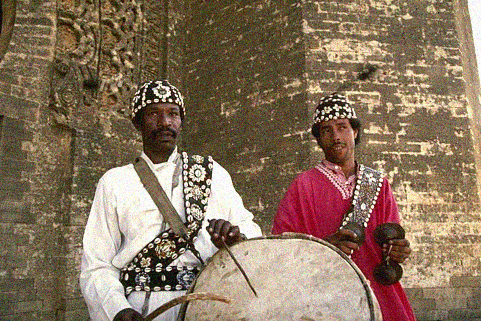
\includegraphics[width=\linewidth]{img/presentazione/noisy/tamburo_noise_15.png}\\[0.3em]
            $\sigma=15$
        \end{minipage} &
        \begin{minipage}{0.28\linewidth}
            \centering
            \textbf{RidNet}\\[0.3em]
            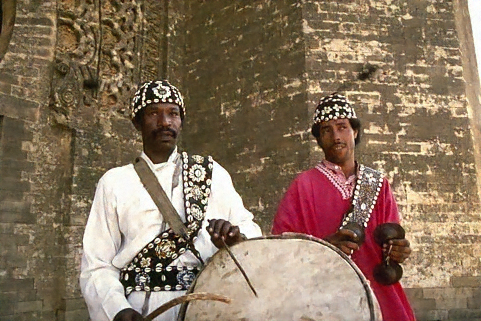
\includegraphics[width=\linewidth]{img/presentazione/ridnet/tamburo_denoise_ridnet_15.png}\\[0.3em]
            PSNR=30.4905
        \end{minipage} &
        \begin{minipage}{0.28\linewidth}
            \centering
            \textbf{DnCNN}\\[0.3em]
            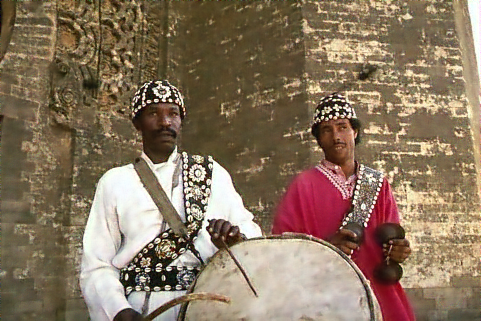
\includegraphics[width=\linewidth]{img/presentazione/dncnn/tamburo_denoise_dncnn_15.png}\\[0.3em]
            PSNR=29.0088
        \end{minipage} \\[1em]
        % Seconda riga: GT, Autoencoder, BM3D
        \begin{minipage}{0.28\linewidth}
            \centering
            \textbf{GT}\\[0.3em]
            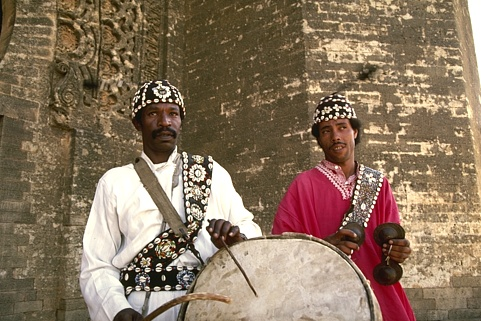
\includegraphics[width=\linewidth]{img/presentazione/bsd_tamburo.jpg}\\[0.3em]
            --
        \end{minipage} &
        \begin{minipage}{0.28\linewidth}
            \centering
            \textbf{Autoencoder}\\[0.3em]
            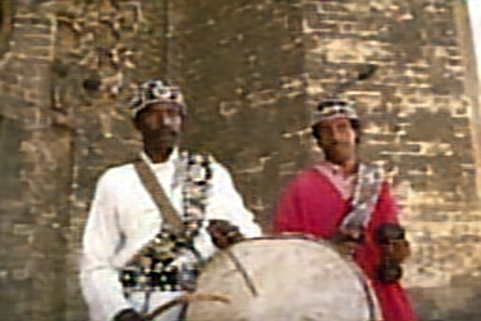
\includegraphics[width=\linewidth]{img/presentazione/autoen/tamburo_denoise_autoen_15.png}\\[0.3em]
            PSNR=23.0973
        \end{minipage} &
        \begin{minipage}{0.28\linewidth}
            \centering
            \textbf{BM3D}\\[0.3em]
            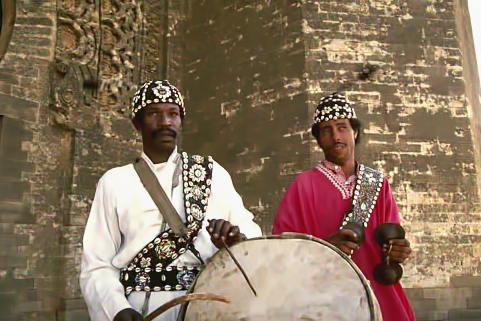
\includegraphics[width=\linewidth]{img/presentazione/bm3d/tamburo_denoise_bm3d_15.png}\\[0.3em]
            PSNR=28.5839
        \end{minipage} \\
    \end{tabular}
\end{frame}

% --- Tamburo σ=25 ---
\begin{frame}{Denoising: $\sigma=25$ (Tamburo)}
    \centering
    \renewcommand{\arraystretch}{1.5}
    \begin{tabular}{c c c}
        \begin{minipage}{0.28\linewidth}
            \centering
            \textbf{Noisy}\\[0.3em]
            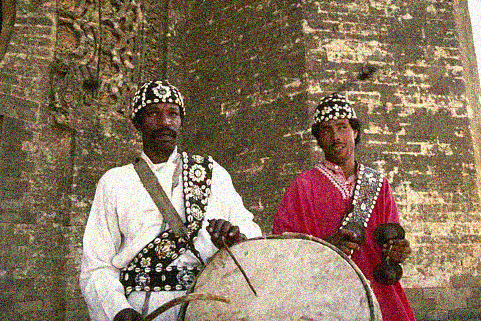
\includegraphics[width=\linewidth]{img/presentazione/noisy/tamburo_noise_25.png}\\[0.3em]
            $\sigma=25$
        \end{minipage} &
        \begin{minipage}{0.28\linewidth}
            \centering
            \textbf{RidNet}\\[0.3em]
            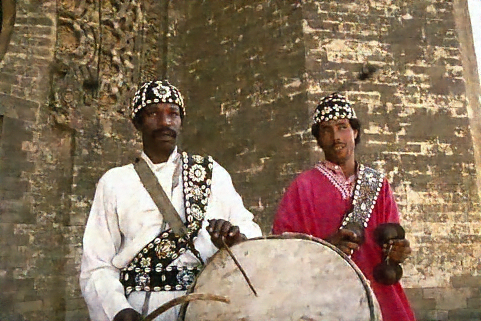
\includegraphics[width=\linewidth]{img/presentazione/ridnet/tamburo_denoise_ridnet_25.png}\\[0.3em]
            PSNR=27.7076
        \end{minipage} &
        \begin{minipage}{0.28\linewidth}
            \centering
            \textbf{DnCNN}\\[0.3em]
            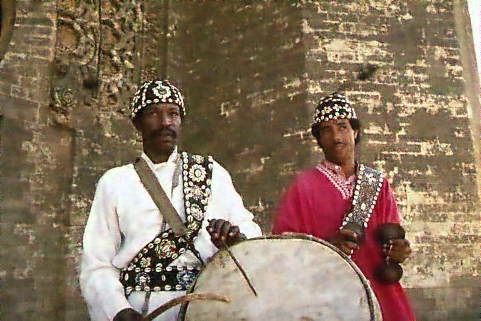
\includegraphics[width=\linewidth]{img/presentazione/dncnn/tamburo_denoise_dncnn_25.png}\\[0.3em]
            PSNR=26.3119
        \end{minipage} \\[1em]
        \begin{minipage}{0.28\linewidth}
            \centering
            \textbf{GT}\\[0.3em]
            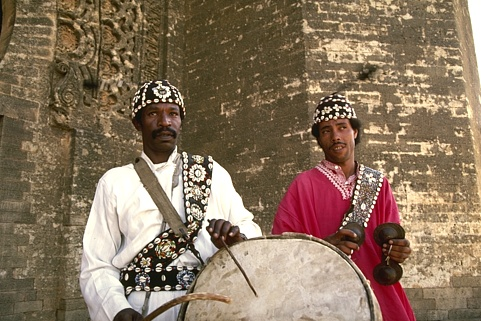
\includegraphics[width=\linewidth]{img/presentazione/bsd_tamburo.jpg}\\[0.3em]
            --
        \end{minipage} &
        \begin{minipage}{0.28\linewidth}
            \centering
            \textbf{Autoencoder}\\[0.3em]
            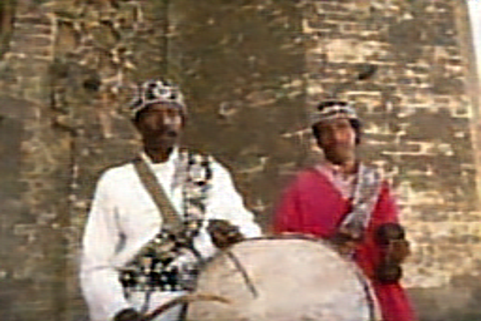
\includegraphics[width=\linewidth]{img/presentazione/autoen/tamburo_denoise_autoen_25.png}\\[0.3em]
            PSNR=22.7748
        \end{minipage} &
        \begin{minipage}{0.28\linewidth}
            \centering
            \textbf{BM3D}\\[0.3em]
            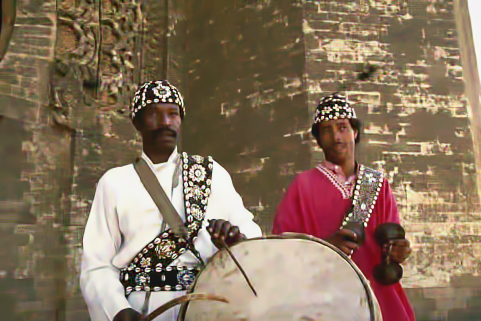
\includegraphics[width=\linewidth]{img/presentazione/bm3d/tamburo_denoise_bm3d_25.png}\\[0.3em]
            PSNR=25.7802
        \end{minipage} \\
    \end{tabular}
\end{frame}

% --- Tamburo σ=50 ---
\begin{frame}{Denoising: $\sigma=50$ (Tamburo)}
    \centering
    \renewcommand{\arraystretch}{1.5}
    \begin{tabular}{c c c}
        \begin{minipage}{0.28\linewidth}
            \centering
            \textbf{Noisy}\\[0.3em]
            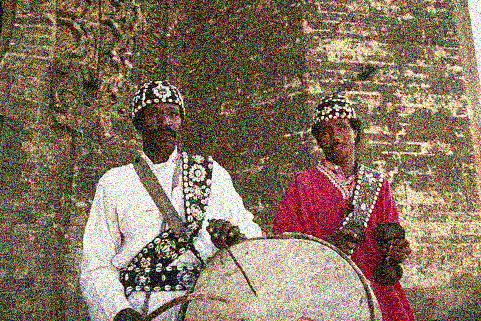
\includegraphics[width=\linewidth]{img/presentazione/noisy/tamburo_noise_50.png}\\[0.3em]
            $\sigma=50$
        \end{minipage} &
        \begin{minipage}{0.28\linewidth}
            \centering
            \textbf{RidNet}\\[0.3em]
            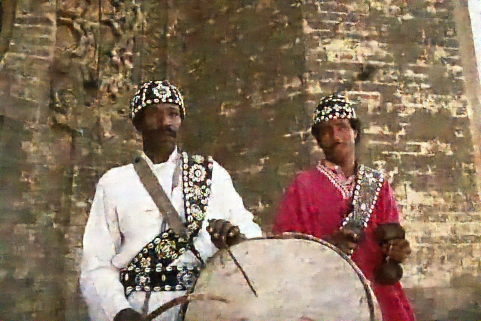
\includegraphics[width=\linewidth]{img/presentazione/ridnet/tamburo_denoise_ridnet_50.png}\\[0.3em]
            PSNR=24.2318
        \end{minipage} &
        \begin{minipage}{0.28\linewidth}
            \centering
            \textbf{DnCNN}\\[0.3em]
            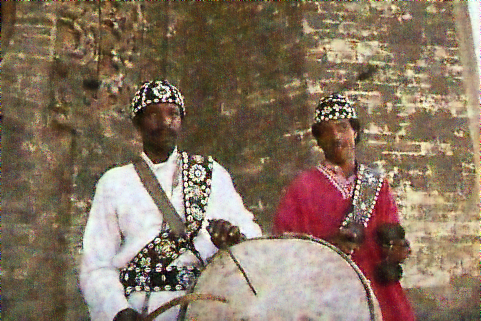
\includegraphics[width=\linewidth]{img/presentazione/dncnn/tamburo_denoise_dncnn_50.png}\\[0.3em]
            PSNR=22.5558
        \end{minipage} \\[1em]
        \begin{minipage}{0.28\linewidth}
            \centering
            \textbf{GT}\\[0.3em]
            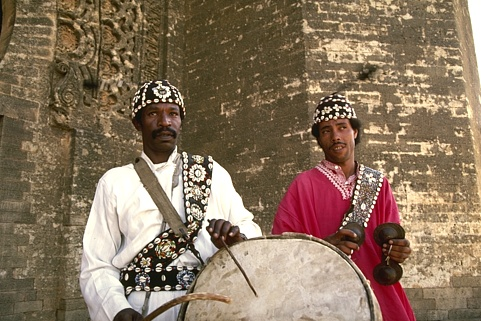
\includegraphics[width=\linewidth]{img/presentazione/bsd_tamburo.jpg}\\[0.3em]
            --
        \end{minipage} &
        \begin{minipage}{0.28\linewidth}
            \centering
            \textbf{Autoencoder}\\[0.3em]
            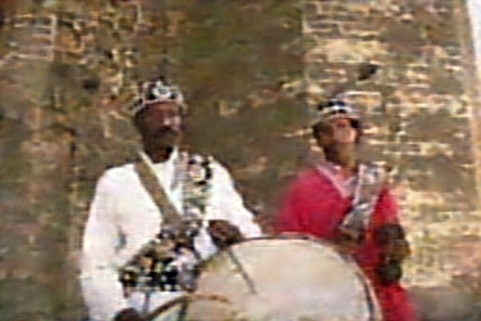
\includegraphics[width=\linewidth]{img/presentazione/autoen/tamburo_denoise_autoen_50.png}\\[0.3em]
            PSNR=21.7567
        \end{minipage} &
        \begin{minipage}{0.28\linewidth}
            \centering
            \textbf{BM3D}\\[0.3em]
            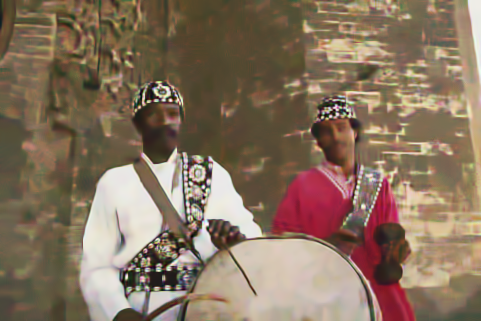
\includegraphics[width=\linewidth]{img/presentazione/bm3d/tamburo_denoise_bm3d_50.png}\\[0.3em]
            PSNR=22.0226
        \end{minipage} \\
    \end{tabular}
\end{frame}



%%%%%%%%%%%%%%%%%% PERSONE  %%%%%%%%%%%%%%%%%%%%%%%%%%%%%%%%%%%%%%%%%%%%%%%%%%%%%%%%%%%%%%%%%%

% --- Denoising σ=15 ---
\begin{frame}{Folla $\sigma=15$}
    \centering
    \renewcommand{\arraystretch}{1.5} % aumenta lo spazio tra le righe
    \begin{tabular}{c c c}
        % Prima riga
        \begin{minipage}{0.28\linewidth}
            \centering
            \textbf{Noisy}\\[0.3em]
            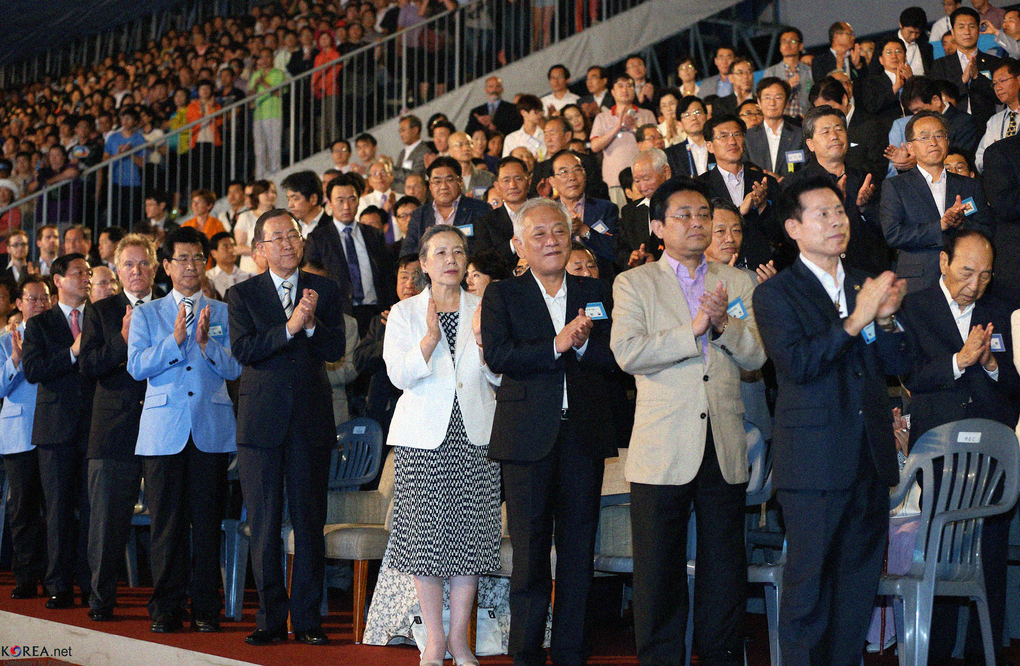
\includegraphics[width=\linewidth]{img/presentazione/noisy/persone_noise_15.png}\\[0.3em]
            $\sigma=15$
        \end{minipage} &
        \begin{minipage}{0.28\linewidth}
            \centering
            \textbf{RidNet}\\[0.3em]
            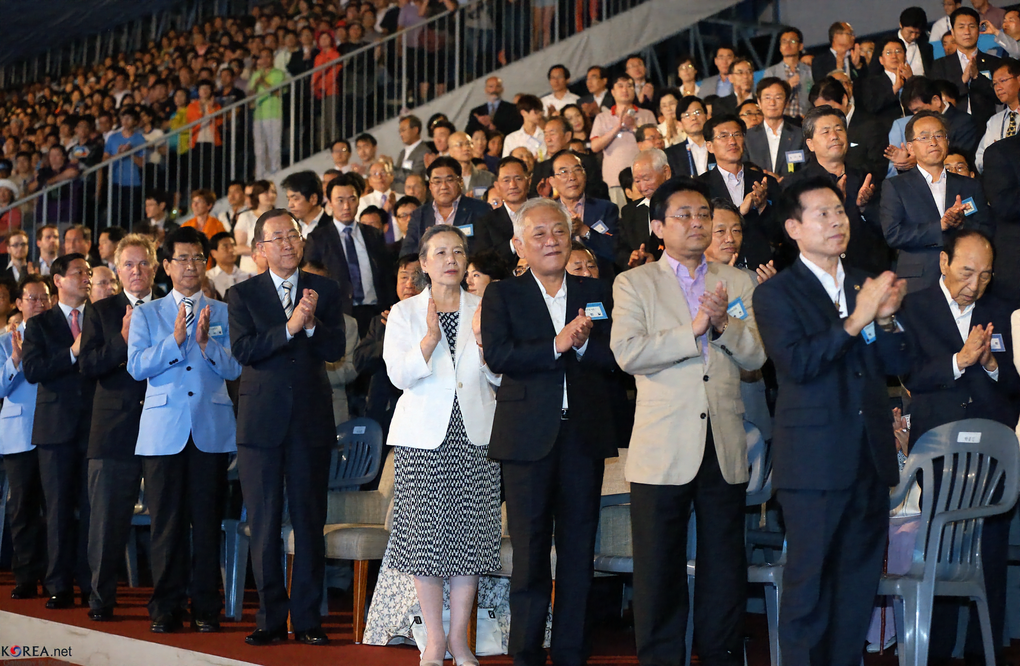
\includegraphics[width=\linewidth]{img/presentazione/ridnet/persone_denoise_ridnet_15.png}\\[0.3em]
            PSNR=34.8141
        \end{minipage} &
        \begin{minipage}{0.28\linewidth}
            \centering
            \textbf{DnCNN}\\[0.3em]
            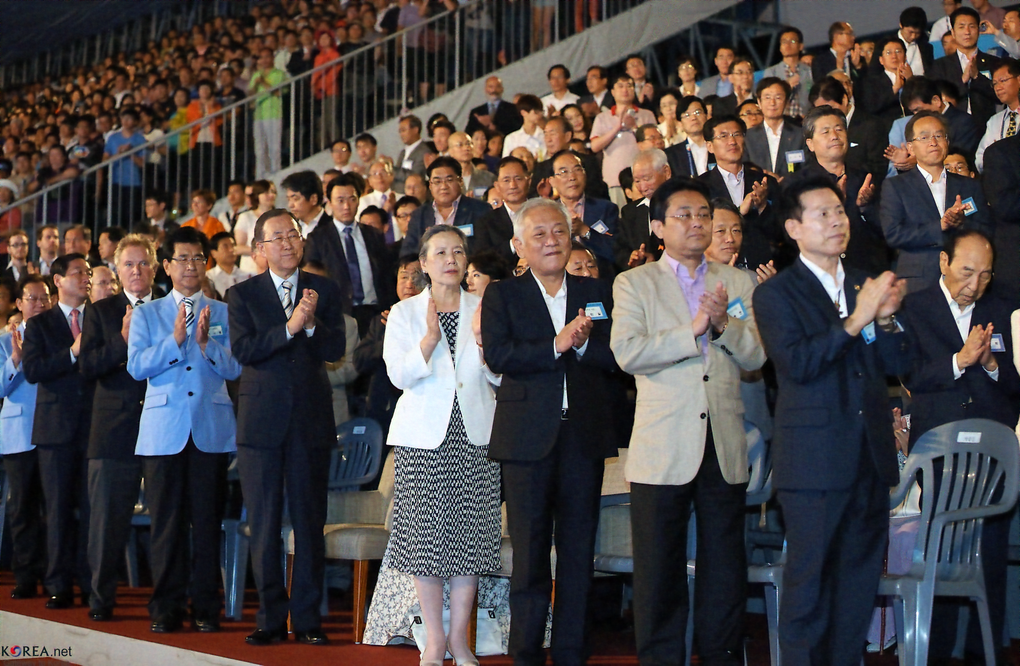
\includegraphics[width=\linewidth]{img/presentazione/dncnn/persone_denoise_dncnn_15.png}\\[0.3em]
            PSNR=32.2842
        \end{minipage} \\[1em]
        % Seconda riga
        \begin{minipage}{0.28\linewidth}
            \centering
            \textbf{GT}\\[0.3em]
            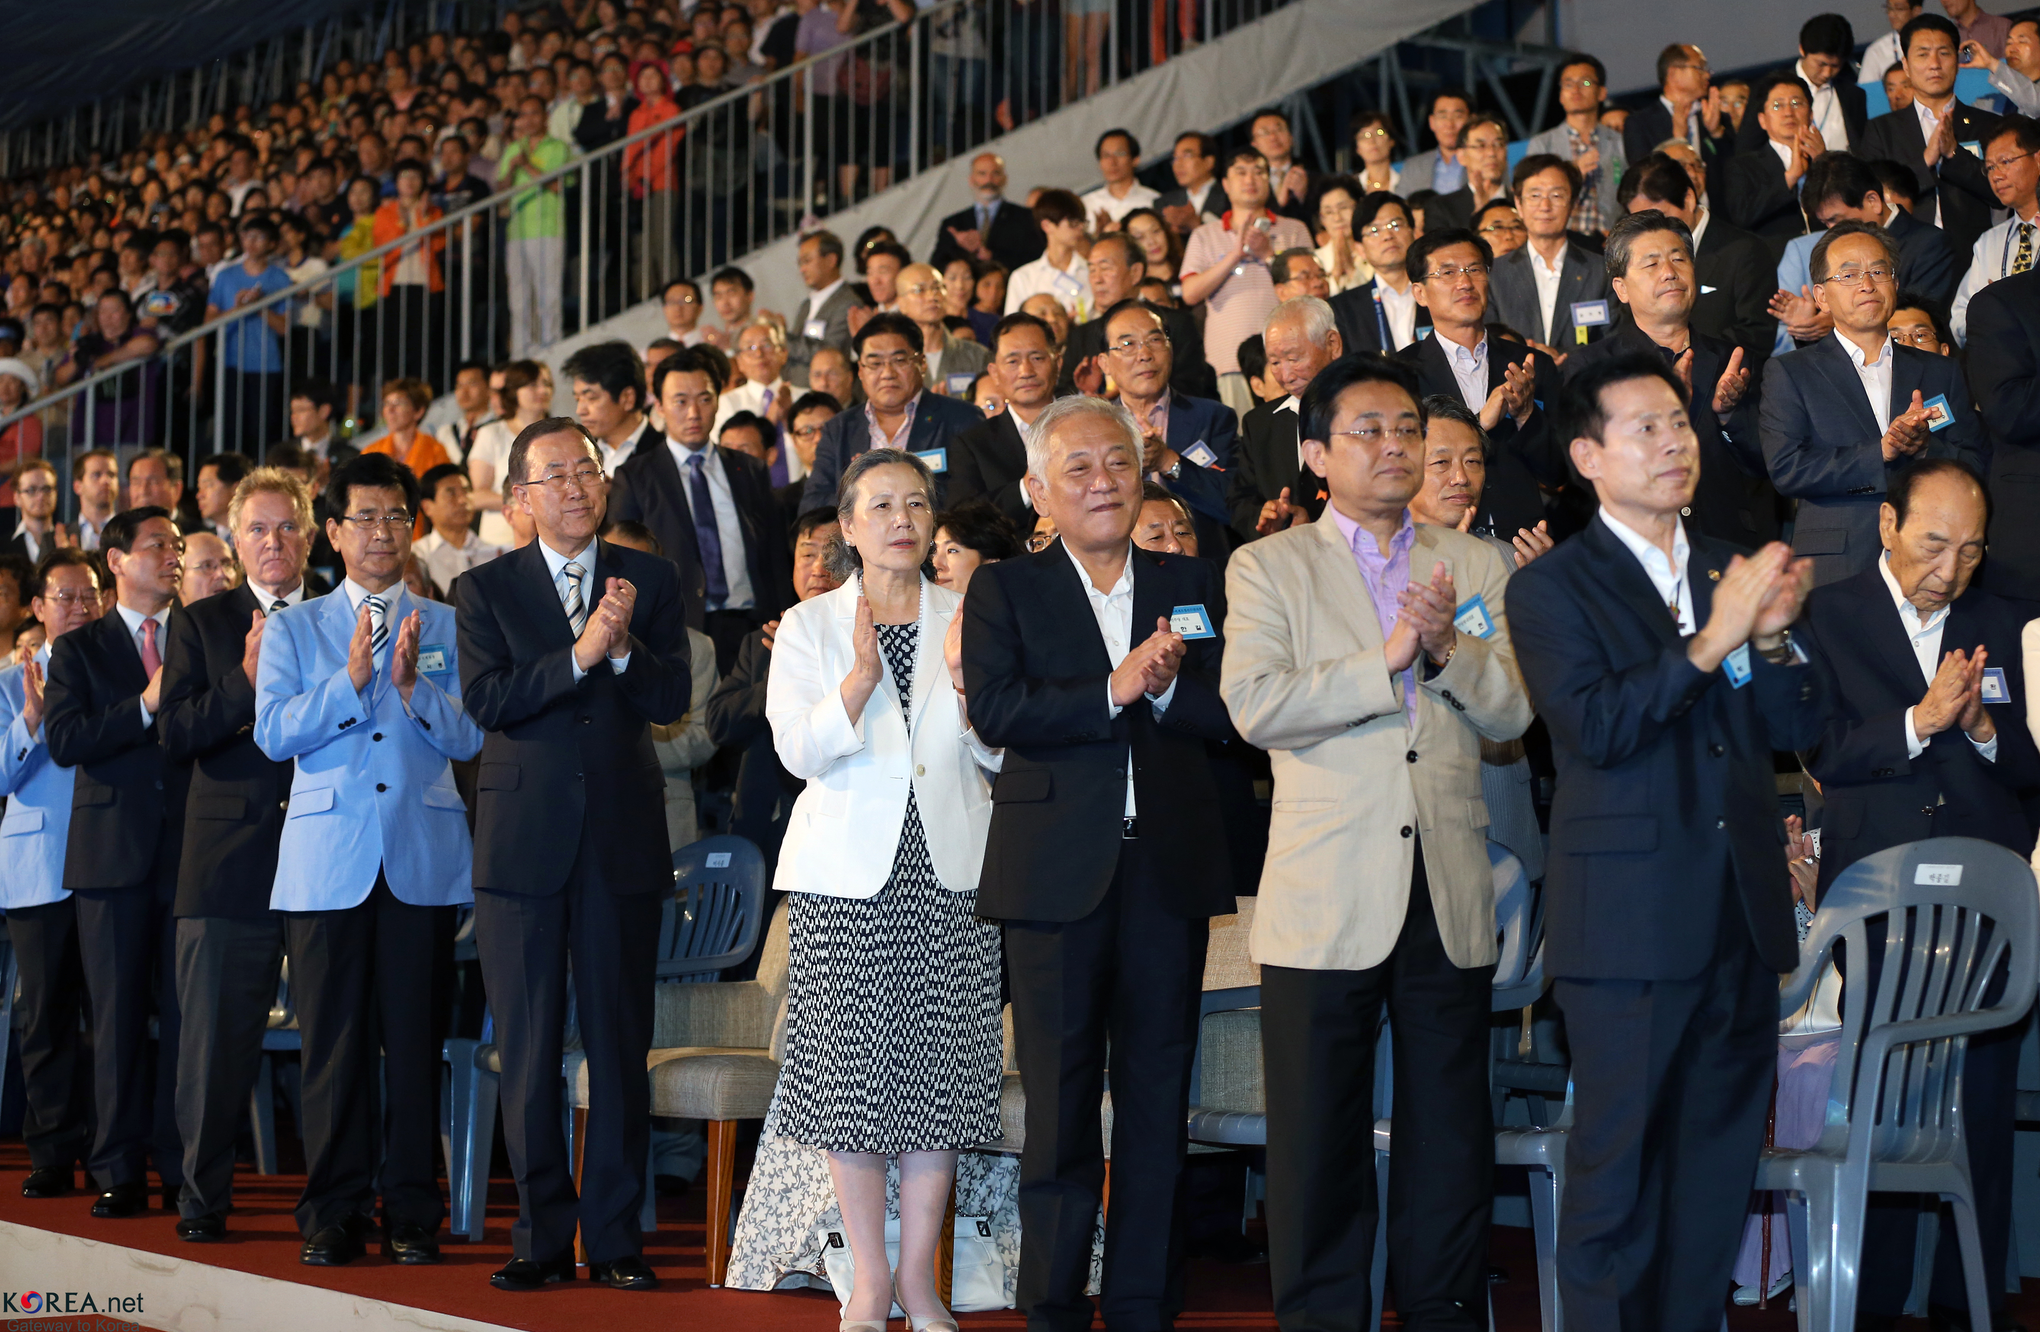
\includegraphics[width=\linewidth]{img/presentazione/div2k_persone.png}\\[0.3em]
            --
        \end{minipage} &
        \begin{minipage}{0.28\linewidth}
            \centering
            \textbf{Autoencoder}\\[0.3em]
            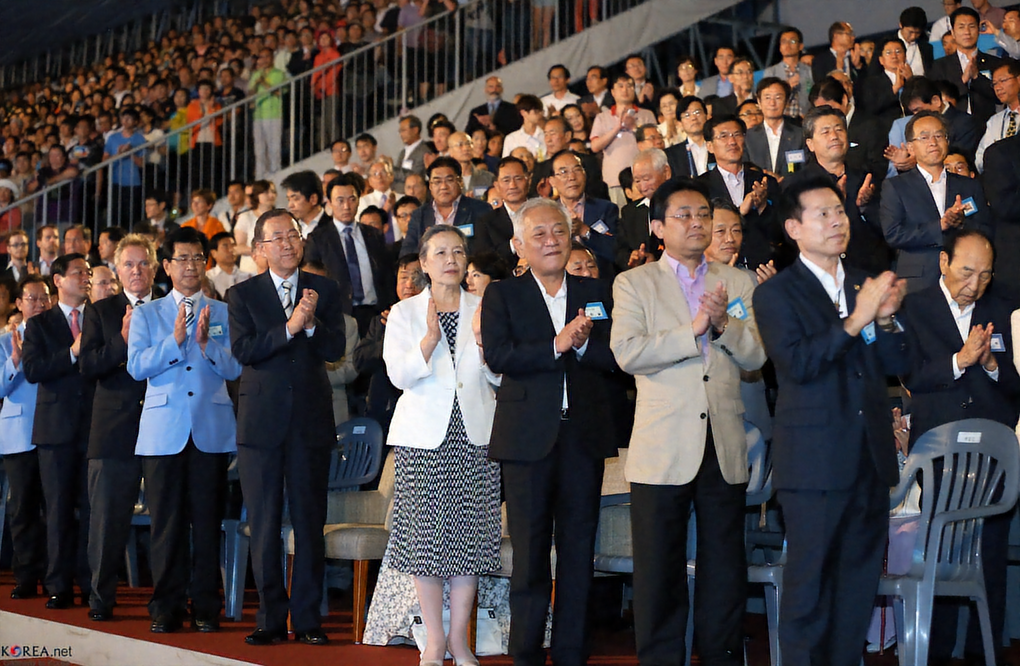
\includegraphics[width=\linewidth]{img/presentazione/autoen/persone_denoise_autoen_15.png}\\[0.3em]
            PSNR=28.3737
        \end{minipage} &
        \begin{minipage}{0.28\linewidth}
            \centering
            \textbf{BM3D}\\[0.3em]
            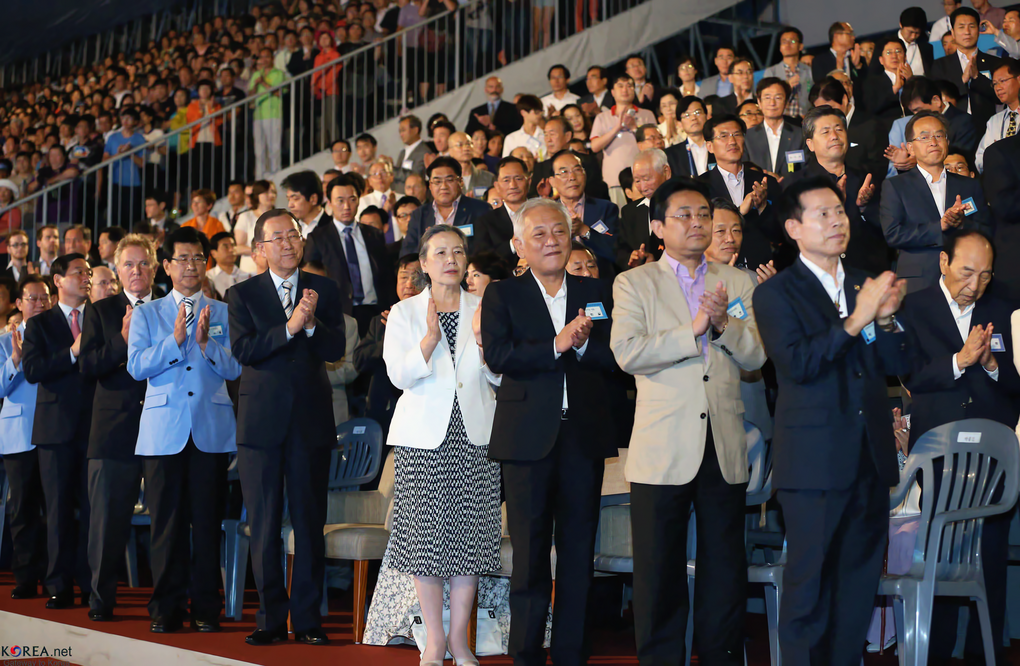
\includegraphics[width=\linewidth]{img/presentazione/bm3d/persone_denoise_bm3d_15.png}\\[0.3em]
            PSNR=34.8250
        \end{minipage} \\
    \end{tabular}
\end{frame}

% --- Denoising σ=25 ---
\begin{frame}{Folla $\sigma=25$}
    \centering
    \renewcommand{\arraystretch}{1.5}
    \begin{tabular}{c c c}
        \begin{minipage}{0.28\linewidth}
            \centering
            \textbf{Noisy}\\[0.3em]
            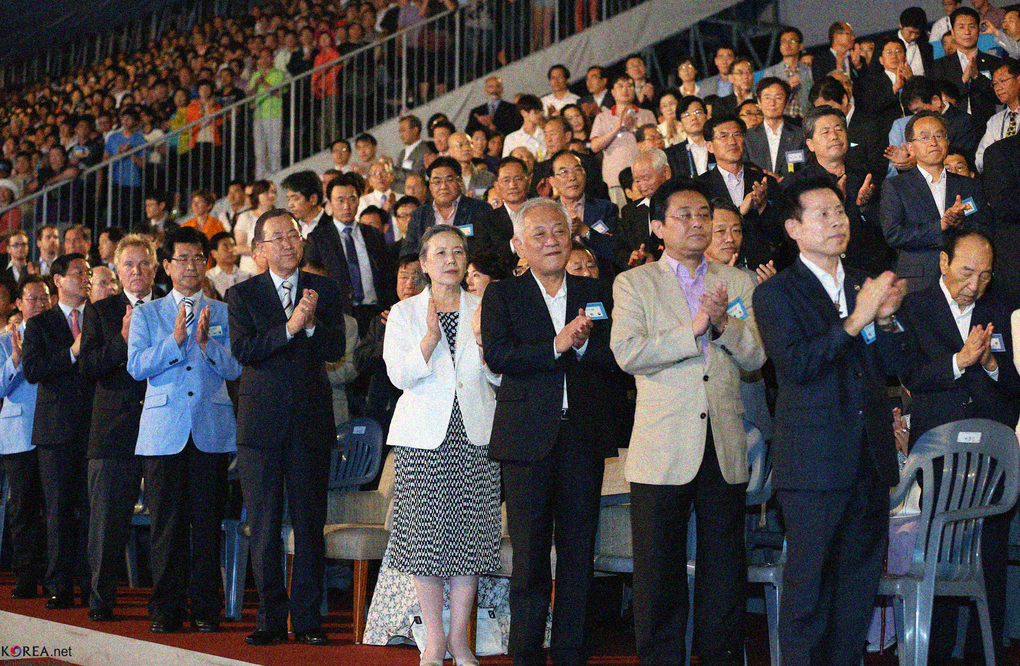
\includegraphics[width=\linewidth]{img/presentazione/noisy/persone_noise_25.png}\\[0.3em]
            $\sigma=25$
        \end{minipage} &
        \begin{minipage}{0.28\linewidth}
            \centering
            \textbf{RidNet}\\[0.3em]
            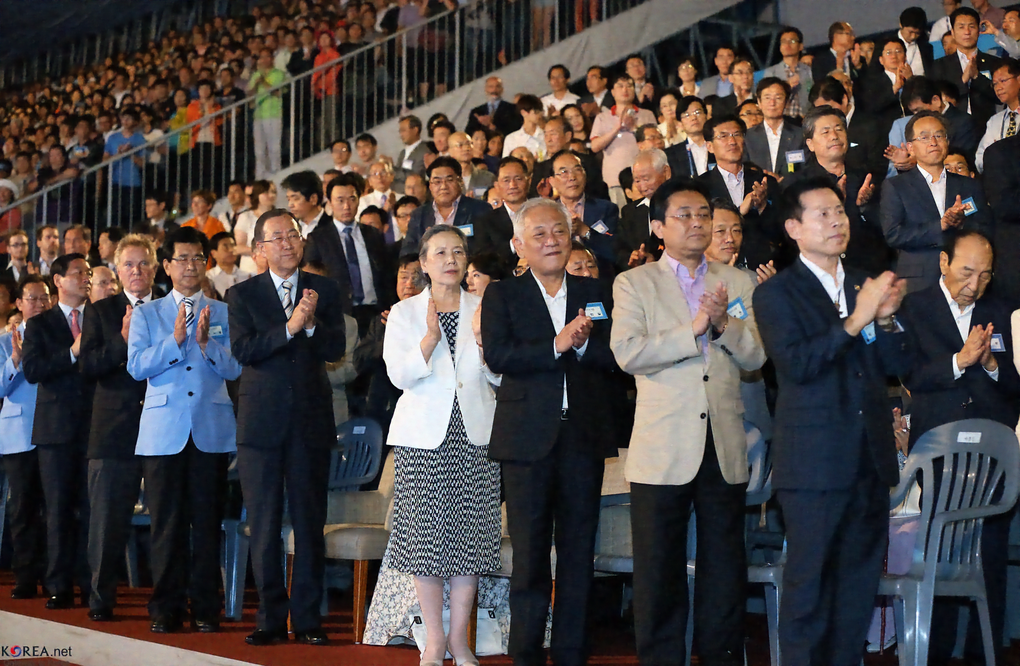
\includegraphics[width=\linewidth]{img/presentazione/ridnet/persone_denoise_ridnet_25.png}\\[0.3em]
            PSNR=32.2756
        \end{minipage} &
        \begin{minipage}{0.28\linewidth}
            \centering
            \textbf{DnCNN}\\[0.3em]
            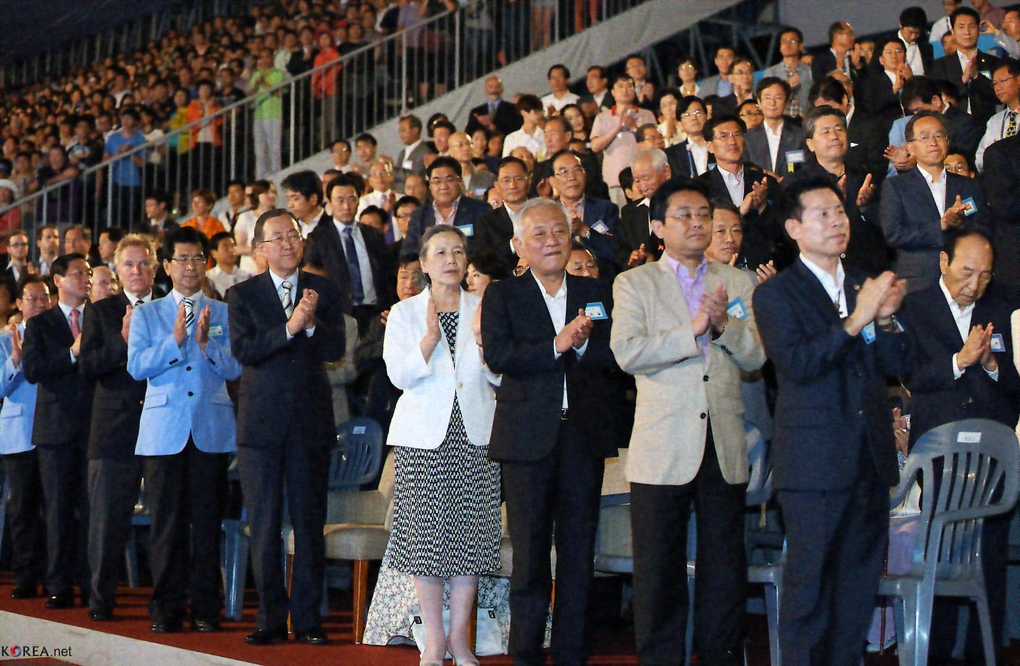
\includegraphics[width=\linewidth]{img/presentazione/dncnn/persone_denoise_dncnn_25.png}\\[0.3em]
            PSNR=30.2877
        \end{minipage} \\[1em]
        \begin{minipage}{0.28\linewidth}
            \centering
            \textbf{GT}\\[0.3em]
            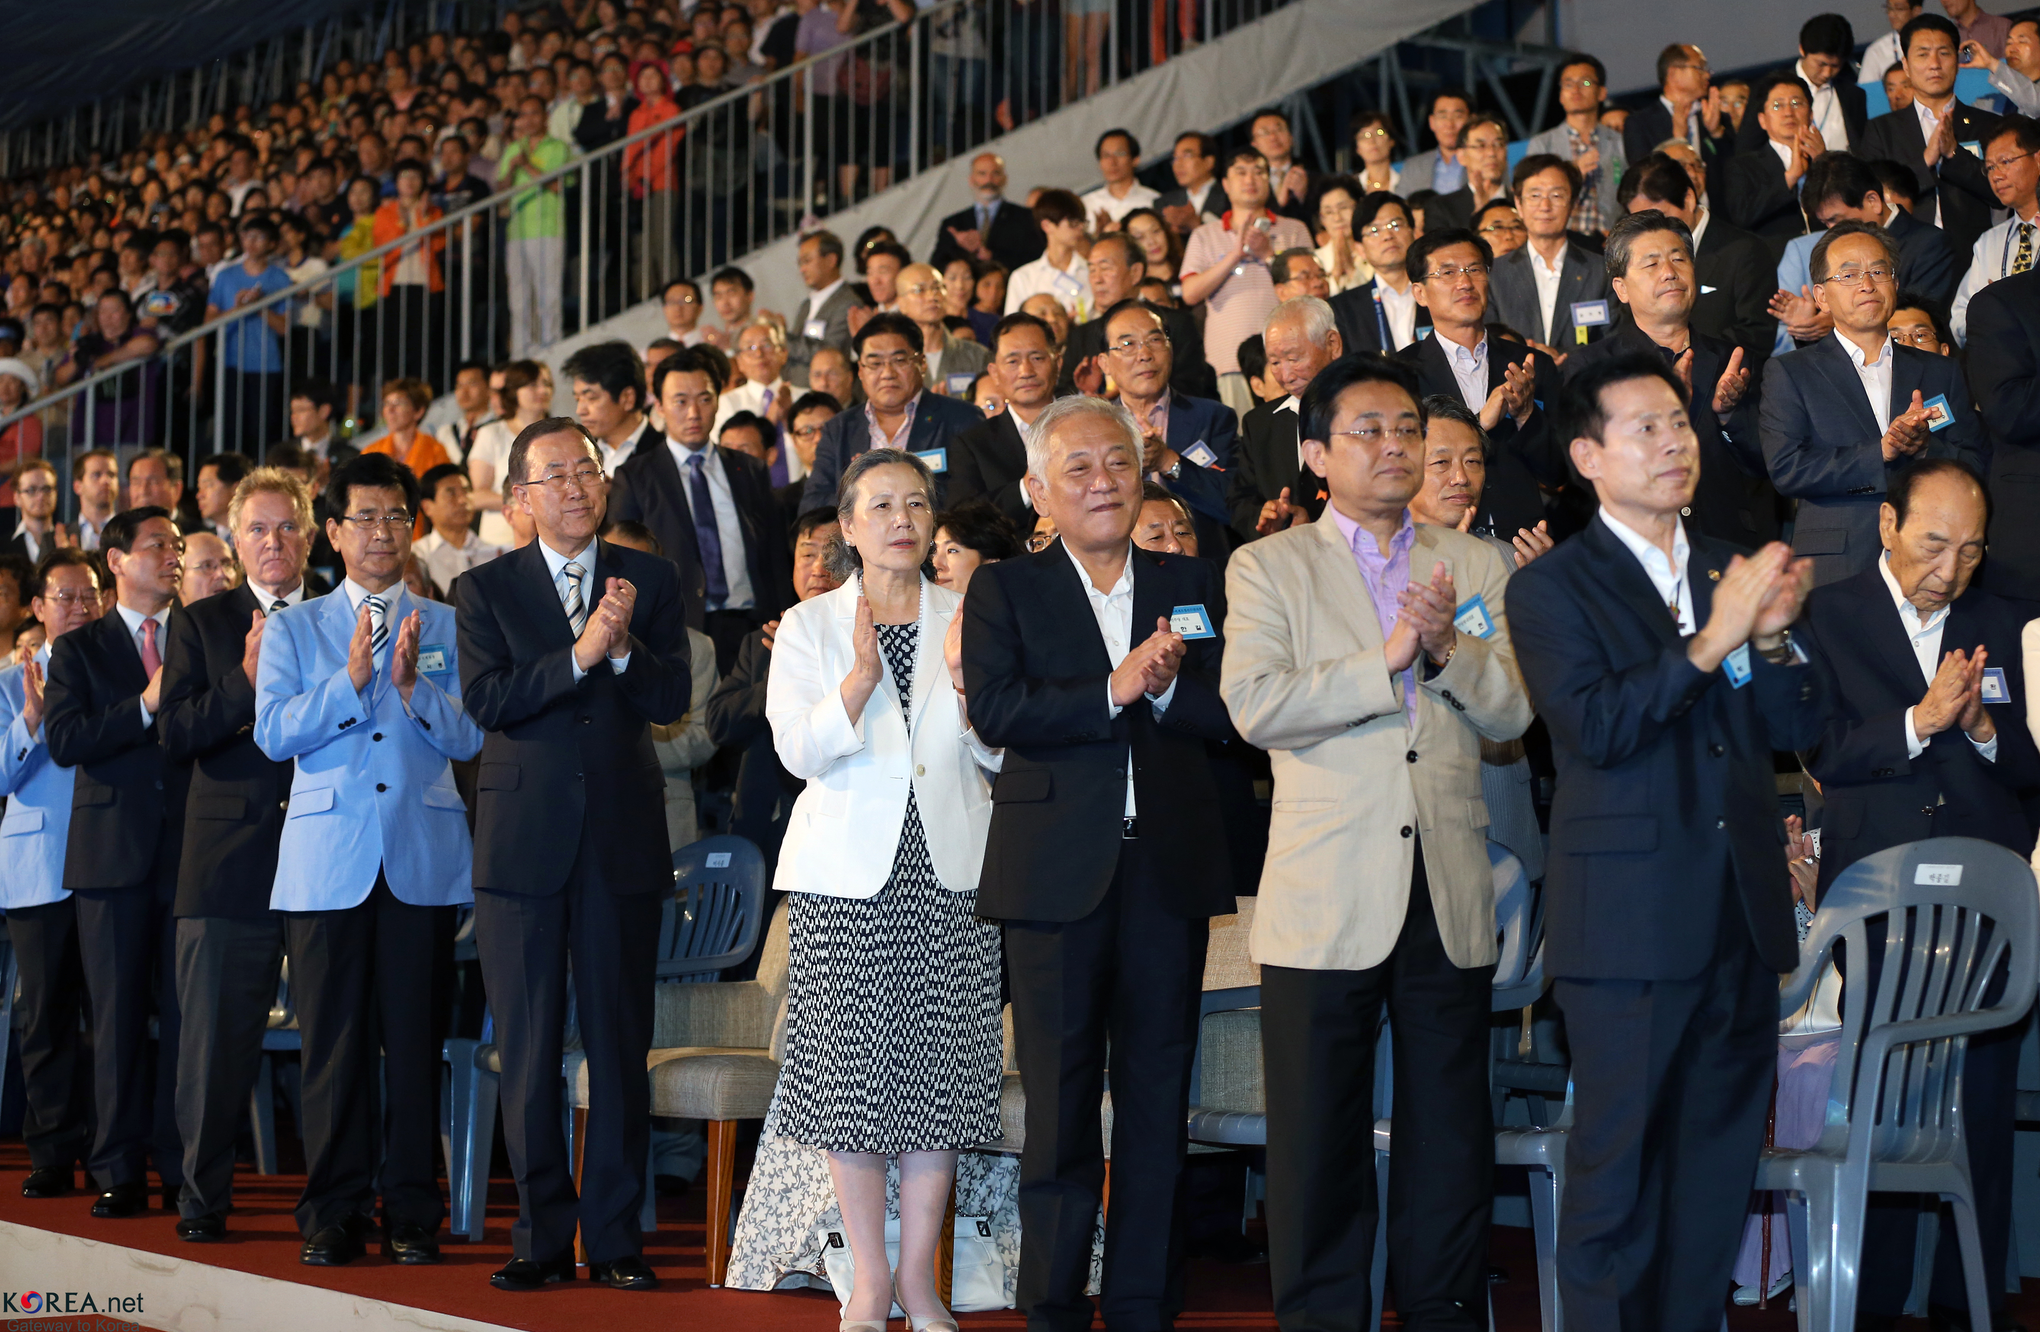
\includegraphics[width=\linewidth]{img/presentazione/div2k_persone.png}\\[0.3em]
            --
        \end{minipage} &
        \begin{minipage}{0.28\linewidth}
            \centering
            \textbf{Autoencoder}\\[0.3em]
            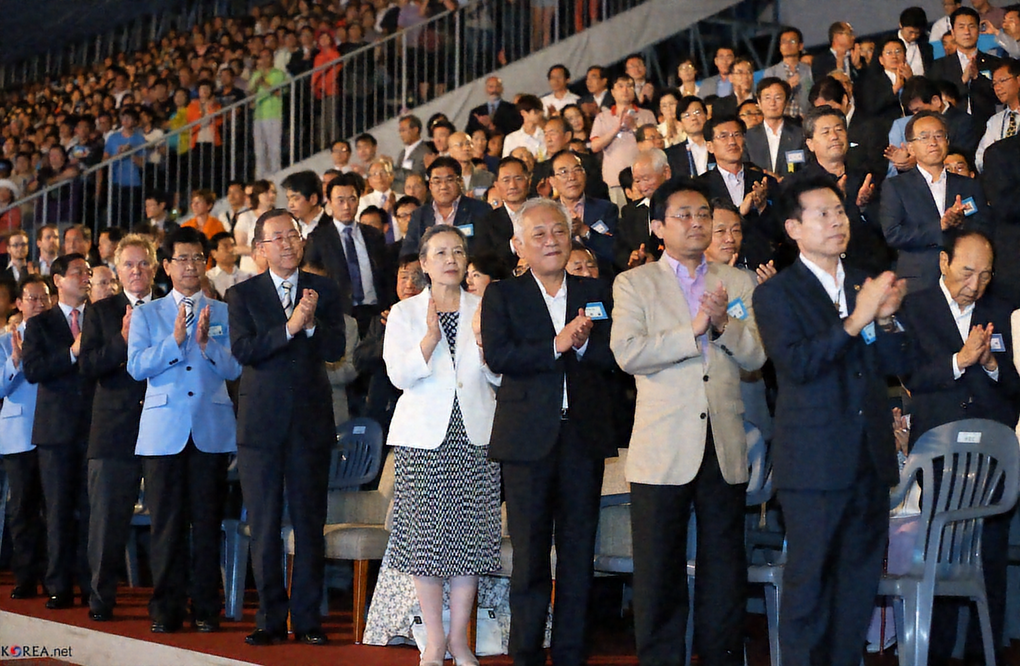
\includegraphics[width=\linewidth]{img/presentazione/autoen/persone_denoise_autoen_25.png}\\[0.3em]
            PSNR=27.7898
        \end{minipage} &
        \begin{minipage}{0.28\linewidth}
            \centering
            \textbf{BM3D}\\[0.3em]
            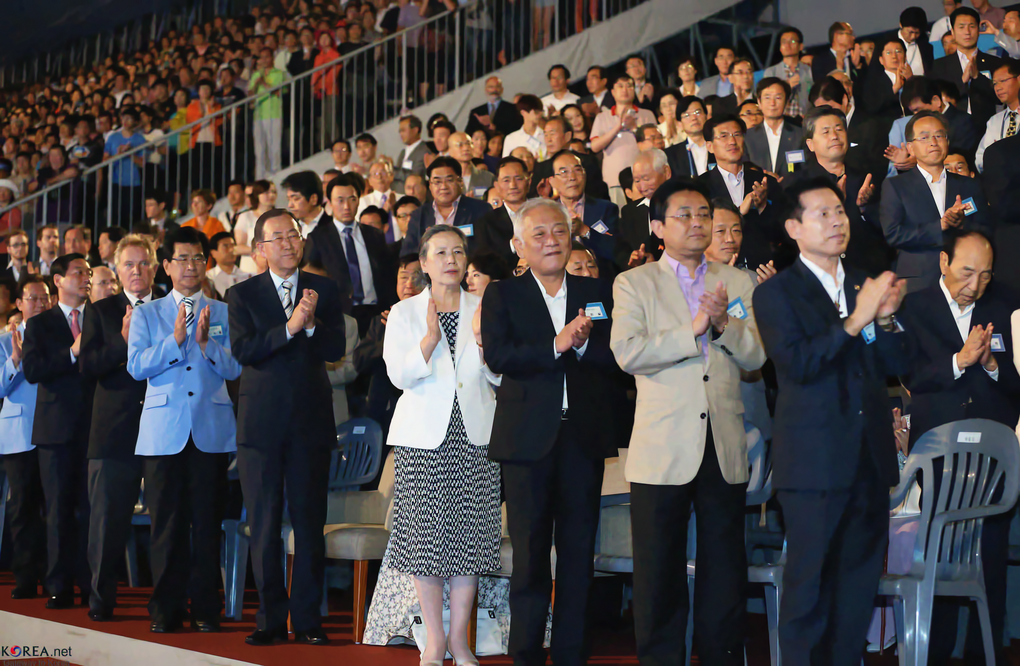
\includegraphics[width=\linewidth]{img/presentazione/bm3d/persone_denoise_bm3d_25.png}\\[0.3em]
            PSNR=31.5916
        \end{minipage} \\
    \end{tabular}
\end{frame}

% --- Denoising σ=50 ---
\begin{frame}{Folla $\sigma=50$}
    \centering
    \renewcommand{\arraystretch}{1.5}
    \begin{tabular}{c c c}
        \begin{minipage}{0.28\linewidth}
            \centering
            \textbf{Noisy}\\[0.3em]
            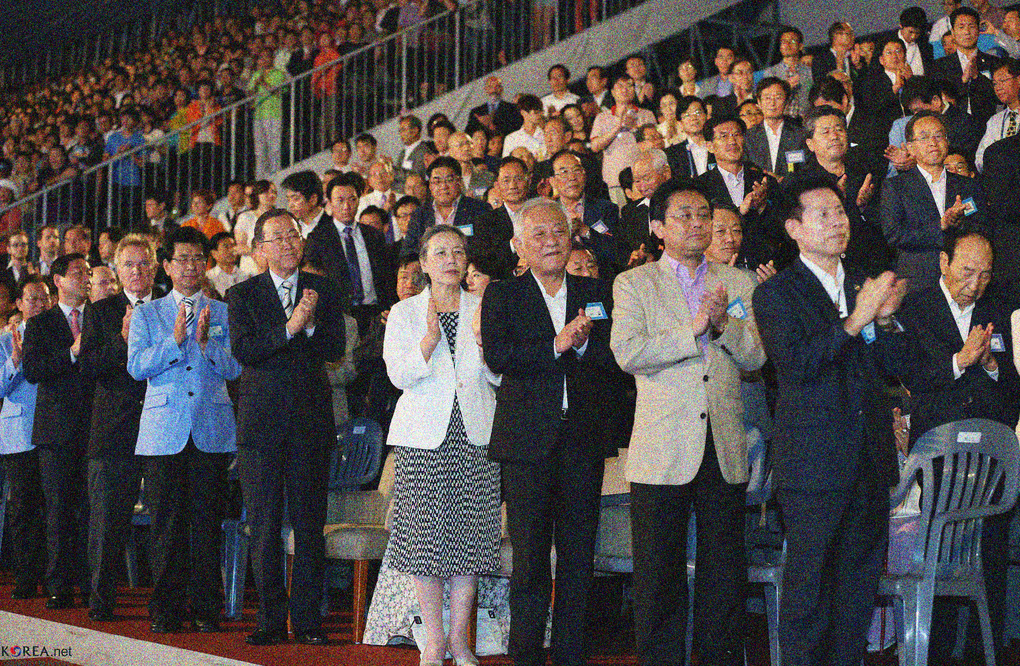
\includegraphics[width=\linewidth]{img/presentazione/noisy/persone_noise_50.png}\\[0.3em]
            $\sigma=50$
        \end{minipage} &
        \begin{minipage}{0.28\linewidth}
            \centering
            \textbf{RidNet}\\[0.3em]
            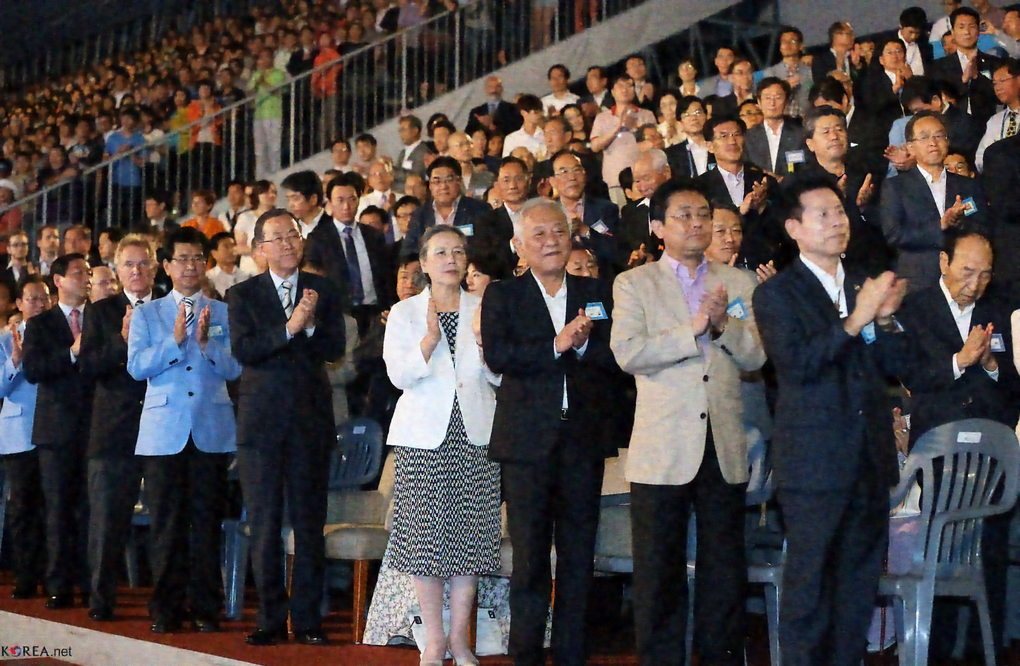
\includegraphics[width=\linewidth]{img/presentazione/ridnet/persone_denoise_ridnet_50.png}\\[0.3em]
            PSNR=28.5562
        \end{minipage} &
        \begin{minipage}{0.28\linewidth}
            \centering
            \textbf{DnCNN}\\[0.3em]
            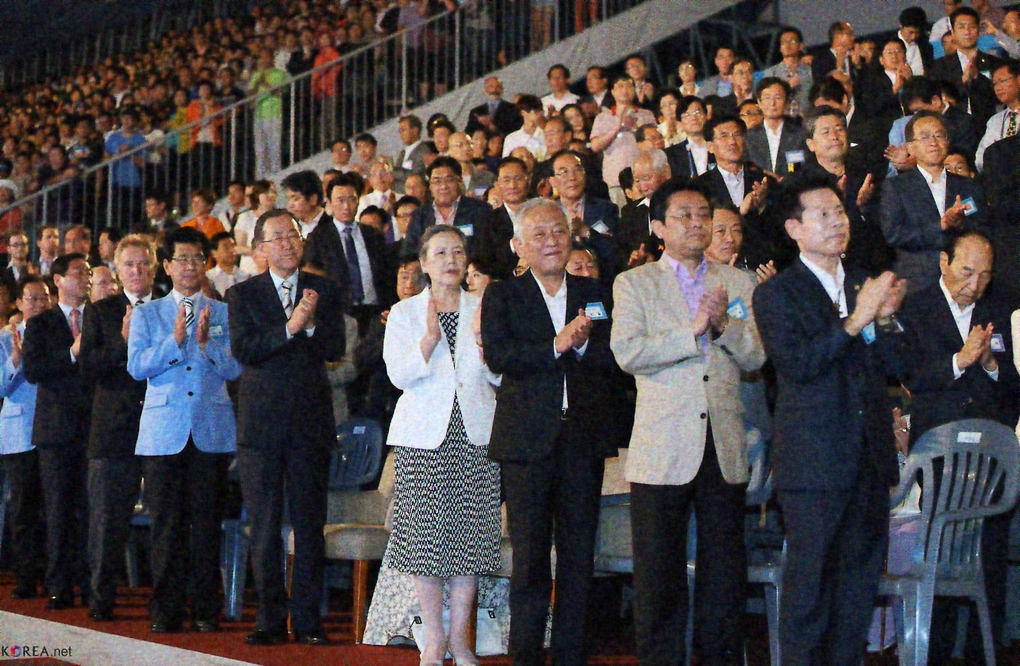
\includegraphics[width=\linewidth]{img/presentazione/dncnn/persone_denoise_dncnn_50.png}\\[0.3em]
            PSNR=26.2250
        \end{minipage} \\[1em]
        \begin{minipage}{0.28\linewidth}
            \centering
            \textbf{GT}\\[0.3em]
            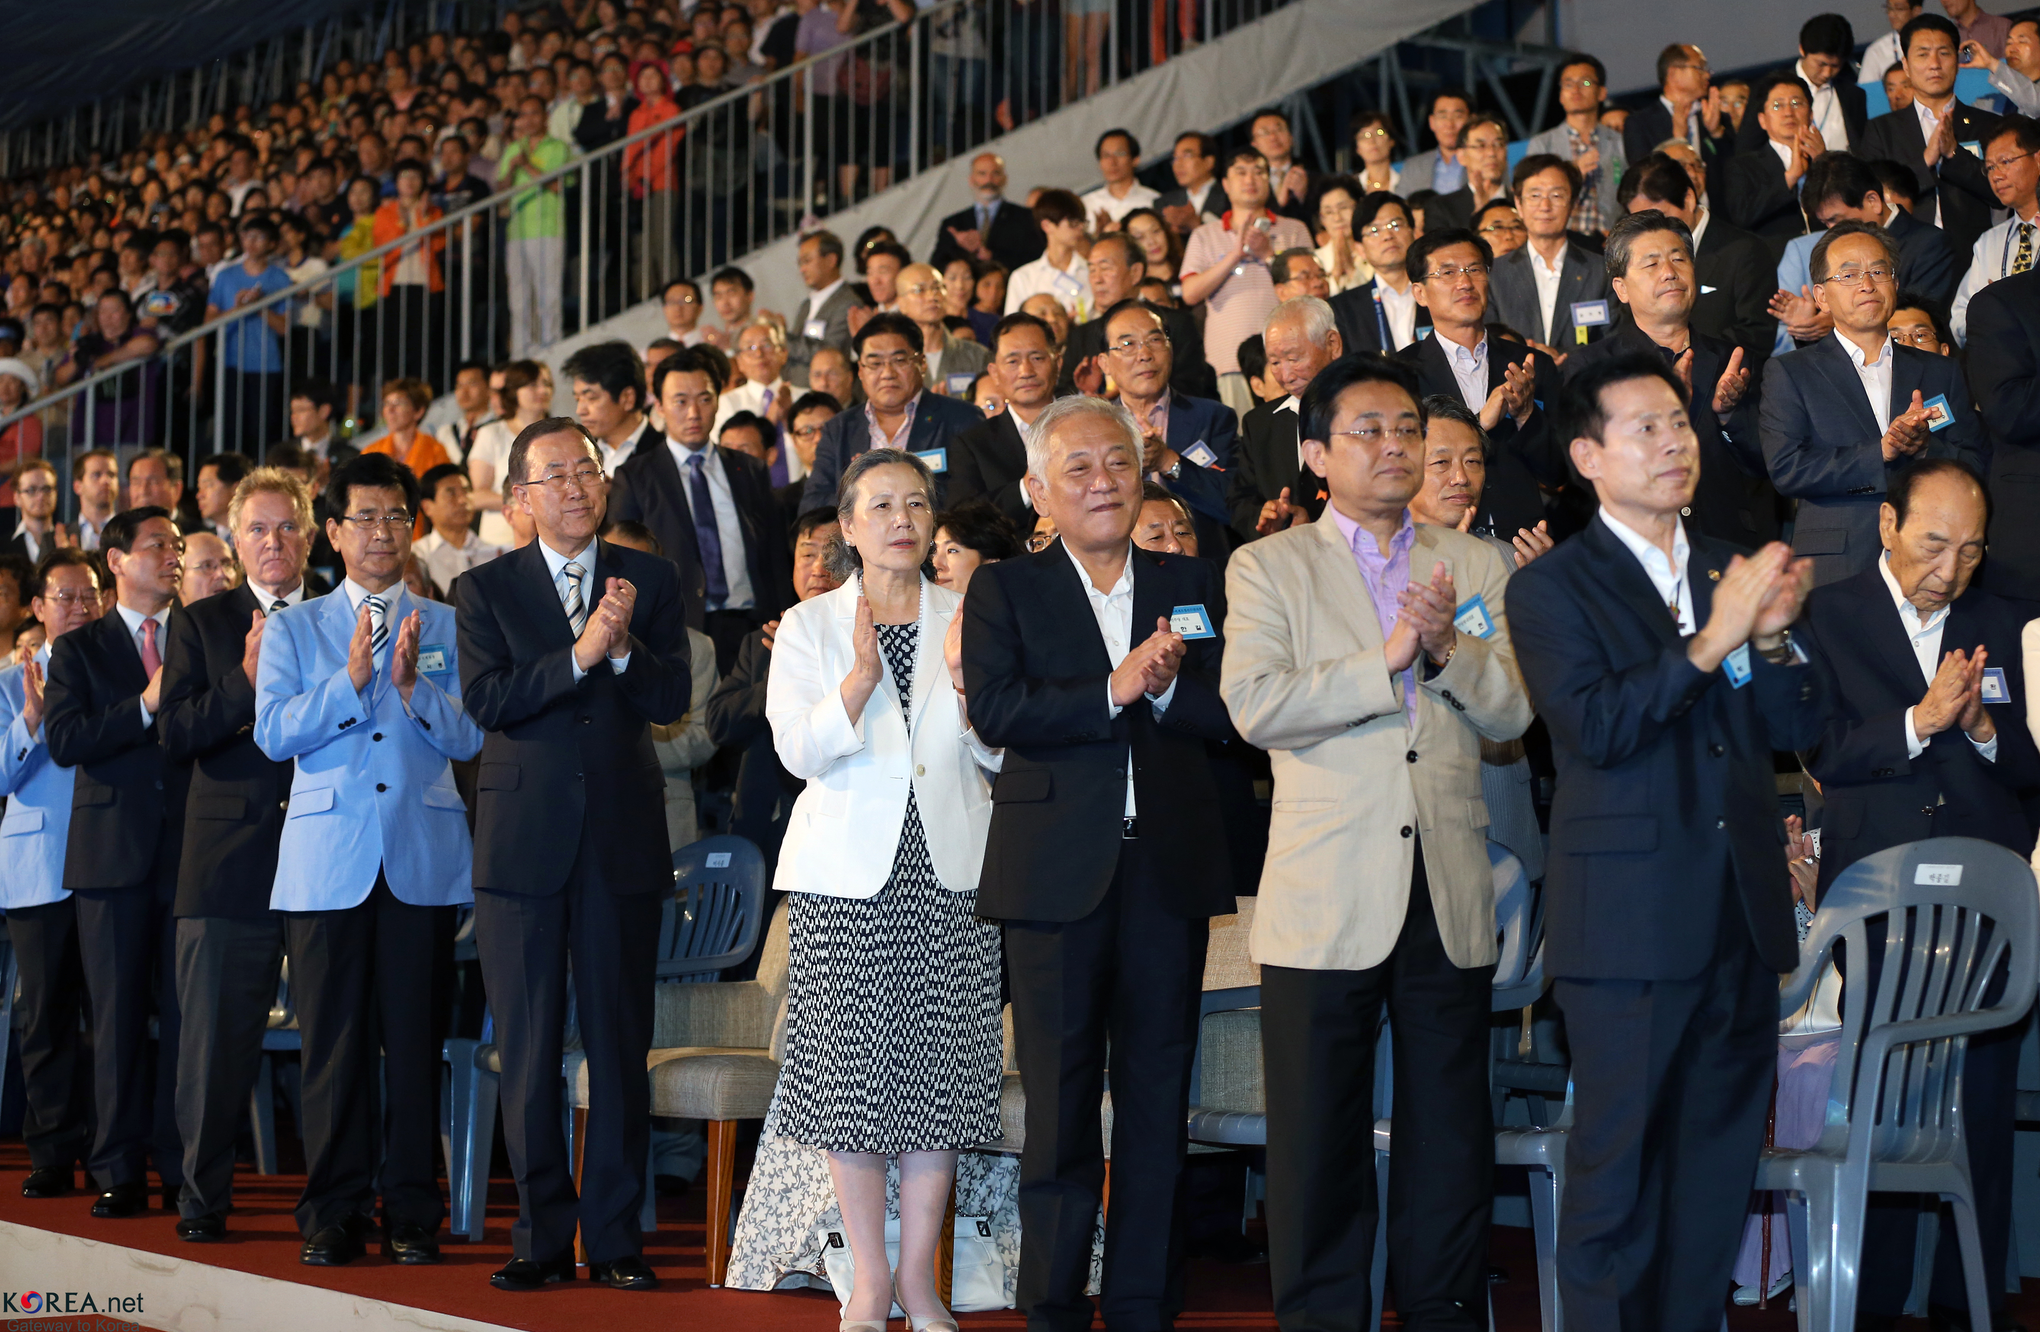
\includegraphics[width=\linewidth]{img/presentazione/div2k_persone.png}\\[0.3em]
            --
        \end{minipage} &
        \begin{minipage}{0.28\linewidth}
            \centering
            \textbf{Autoencoder}\\[0.3em]
            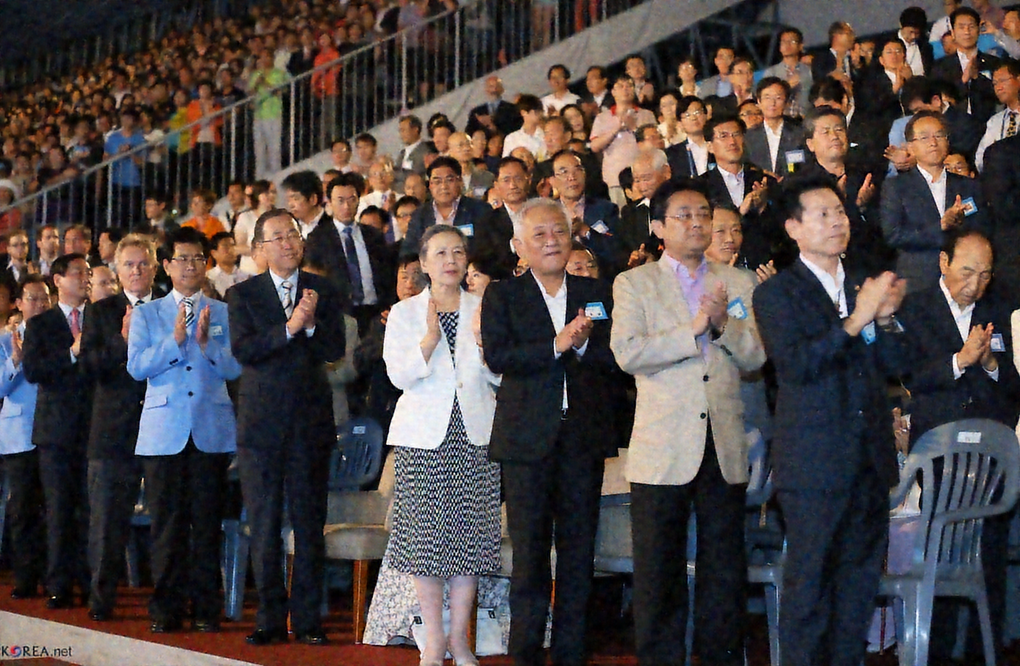
\includegraphics[width=\linewidth]{img/presentazione/autoen/persone_denoise_autoen_50.png}\\[0.3em]
            PSNR=26.3292
        \end{minipage} &
        \begin{minipage}{0.28\linewidth}
            \centering
            \textbf{BM3D}\\[0.3em]
            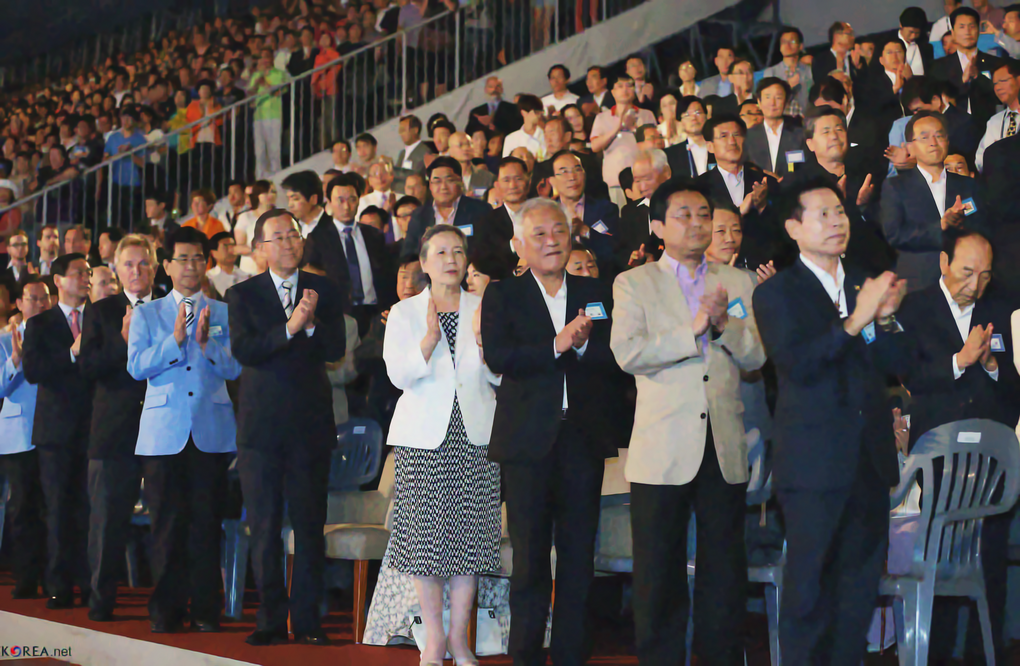
\includegraphics[width=\linewidth]{img/presentazione/bm3d/persone_denoise_bm3d_50.png}\\[0.3em]
            PSNR=26.0076
        \end{minipage} \\
    \end{tabular}
\end{frame}


%%%%%%%%%%%%%%%%%% SCACCHI  %%%%%%%%%%%%%%%%%%%%%%%%%%%%%%%%%%%%%%%%%%%%%%%%%%%%%%%%%%%%%%%%%%


% --- Scacchi σ≈16.473 ---
\begin{frame}{Denoising: Scacchi ($\sigma \approx 16.47$)}
    \centering
    \renewcommand{\arraystretch}{1.5} % aumenta lo spazio tra le righe
    \begin{tabular}{c c c}
        % Prima riga: Noisy, RidNet, DnCNN
        \begin{minipage}{0.28\linewidth}
            \centering
            \textbf{Noisy}\\[0.3em]
            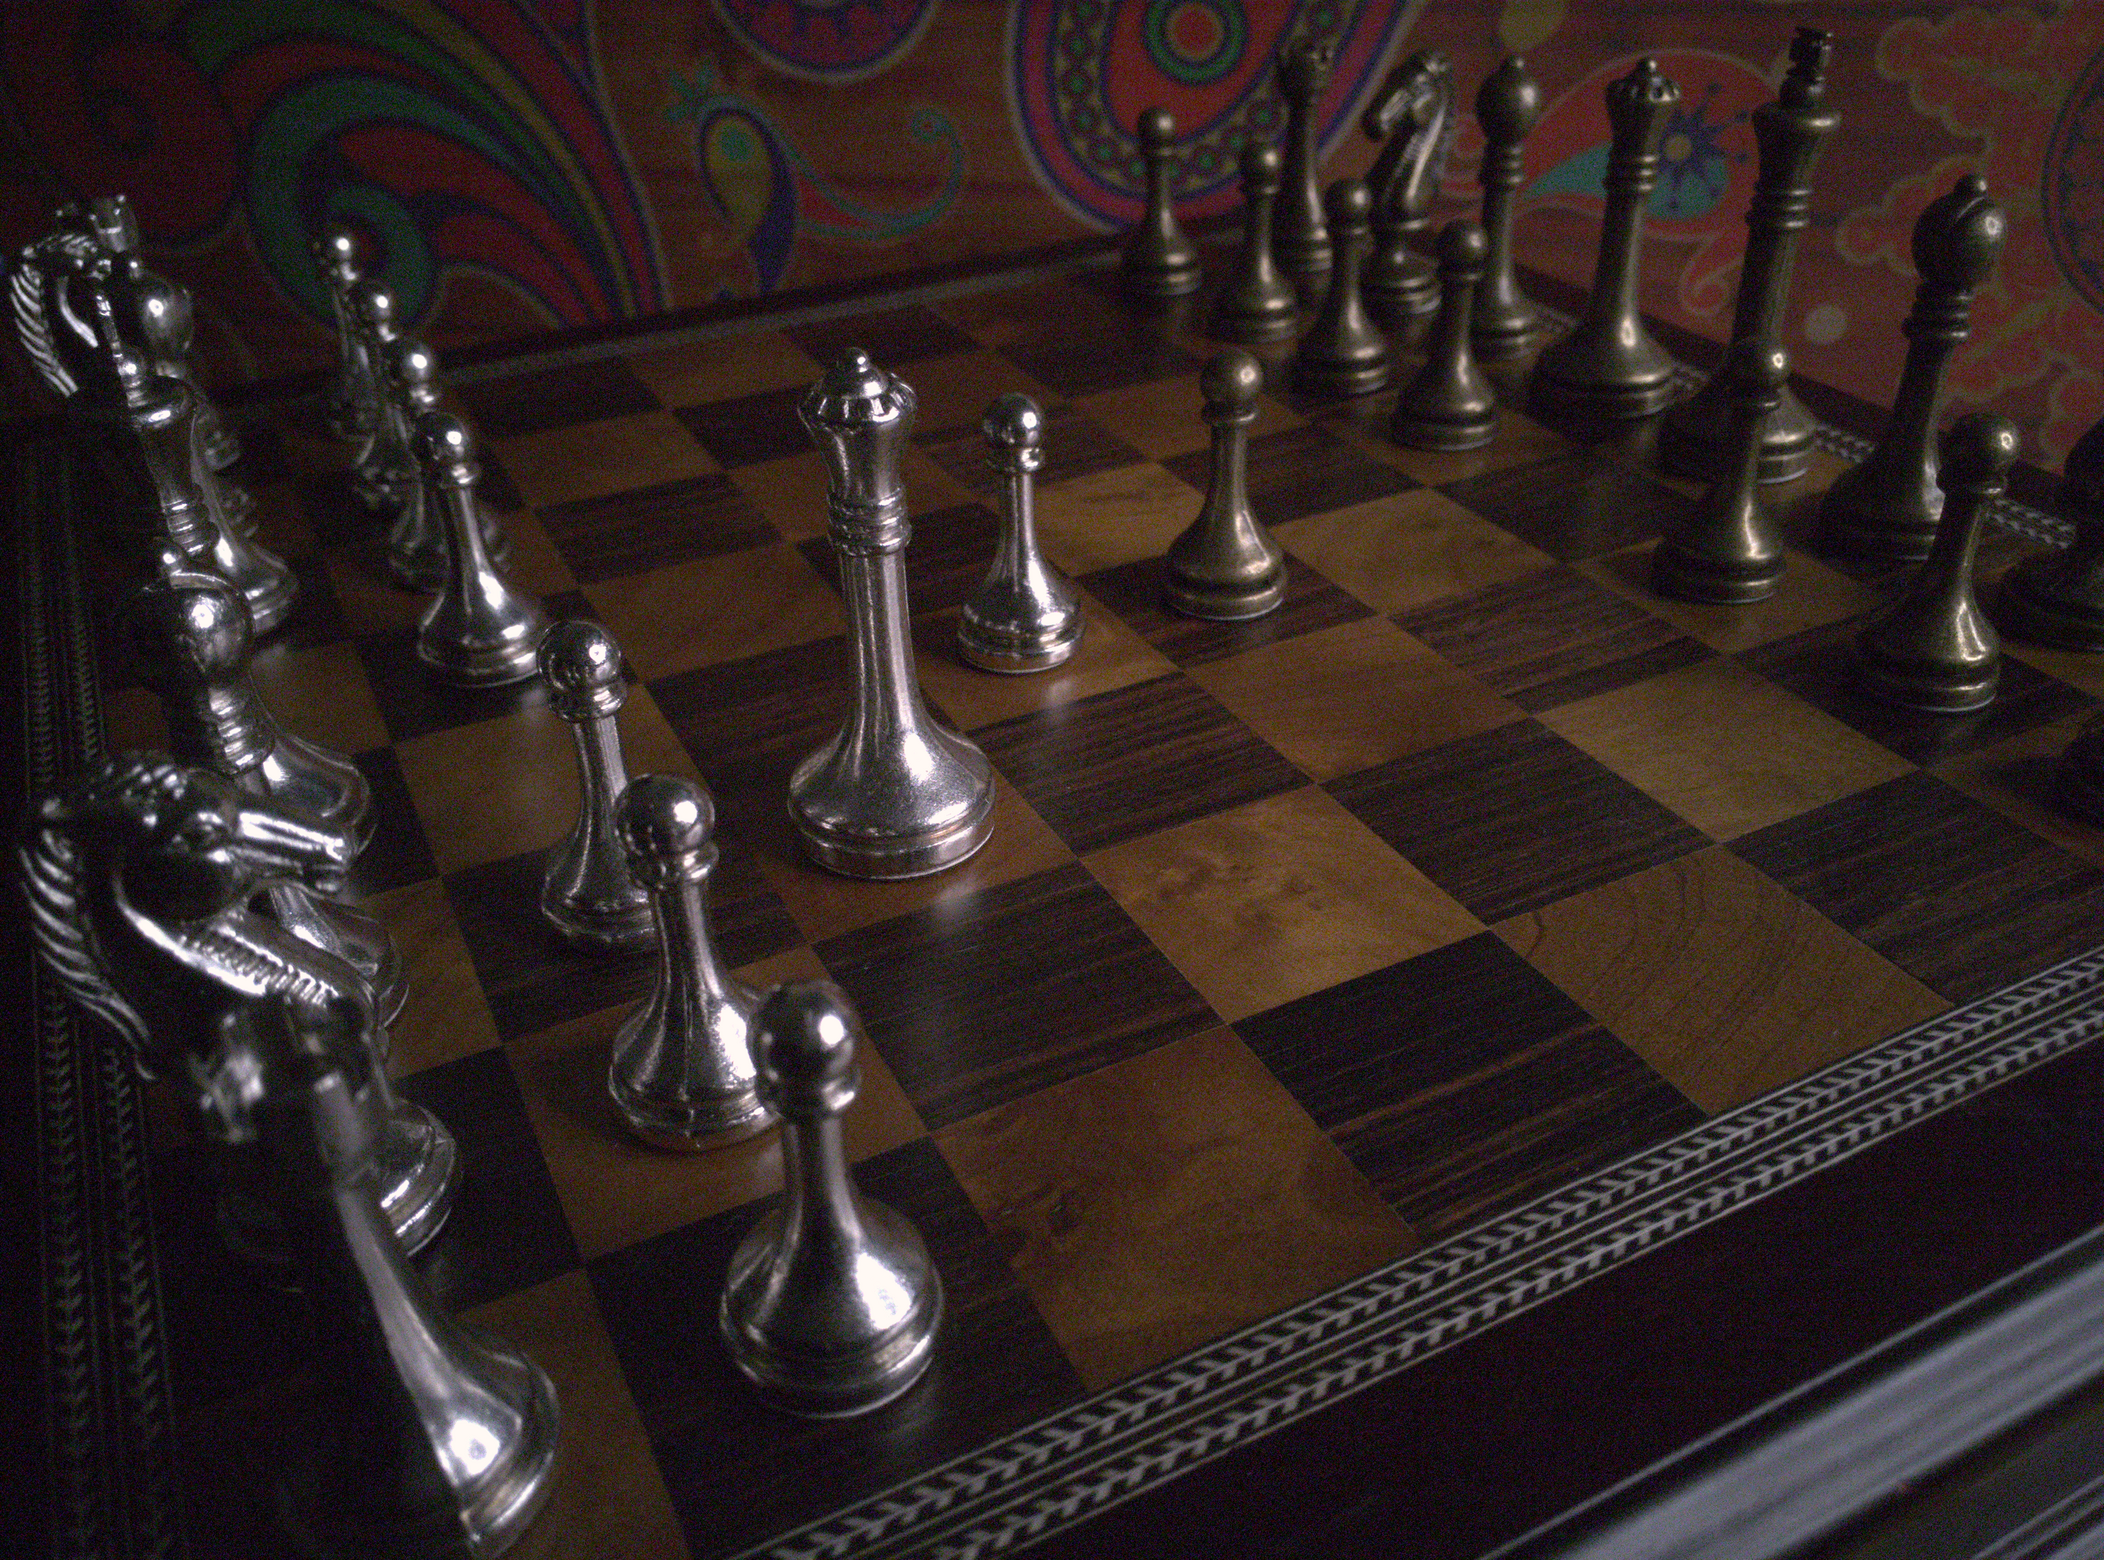
\includegraphics[width=\linewidth]{img/presentazione/sidd_scacchi_noise.PNG}\\[0.3em]
            $\sigma \approx 16.47$
        \end{minipage} &
        \begin{minipage}{0.28\linewidth}
            \centering
            \textbf{RidNet}\\[0.3em]
            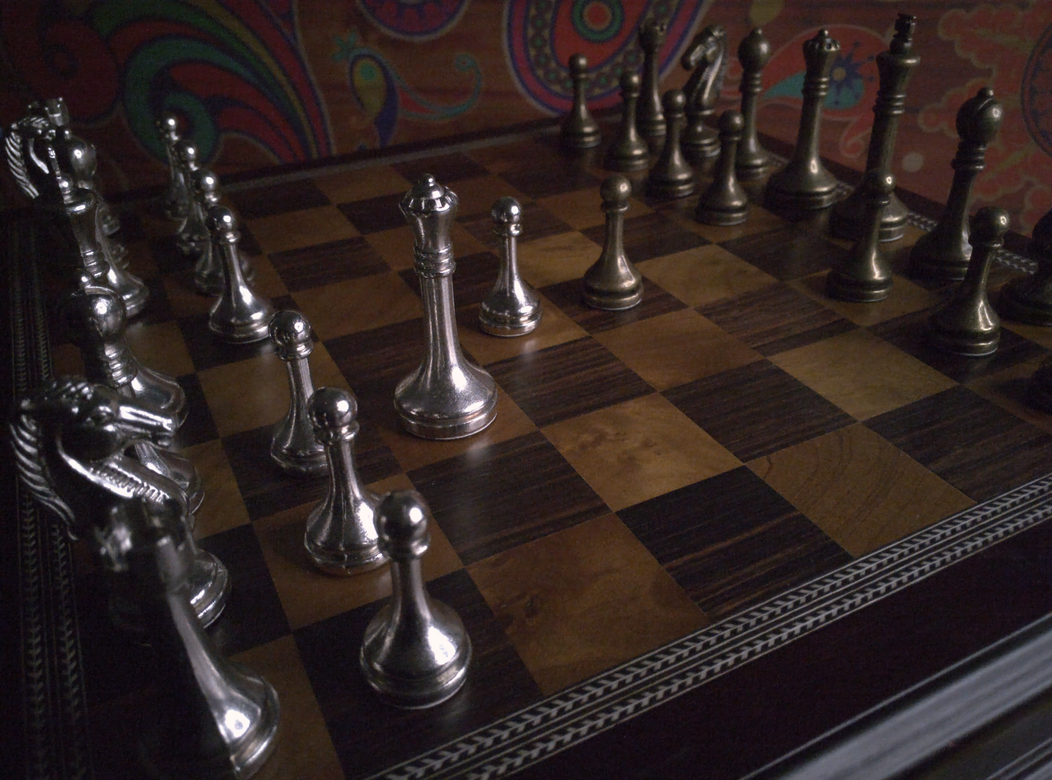
\includegraphics[width=\linewidth]{img/presentazione/ridnet/scacchi_denoise_ridnet.png}\\[0.3em]
            PSNR=34.4284
        \end{minipage} &
        \begin{minipage}{0.28\linewidth}
            \centering
            \textbf{DnCNN}\\[0.3em]
            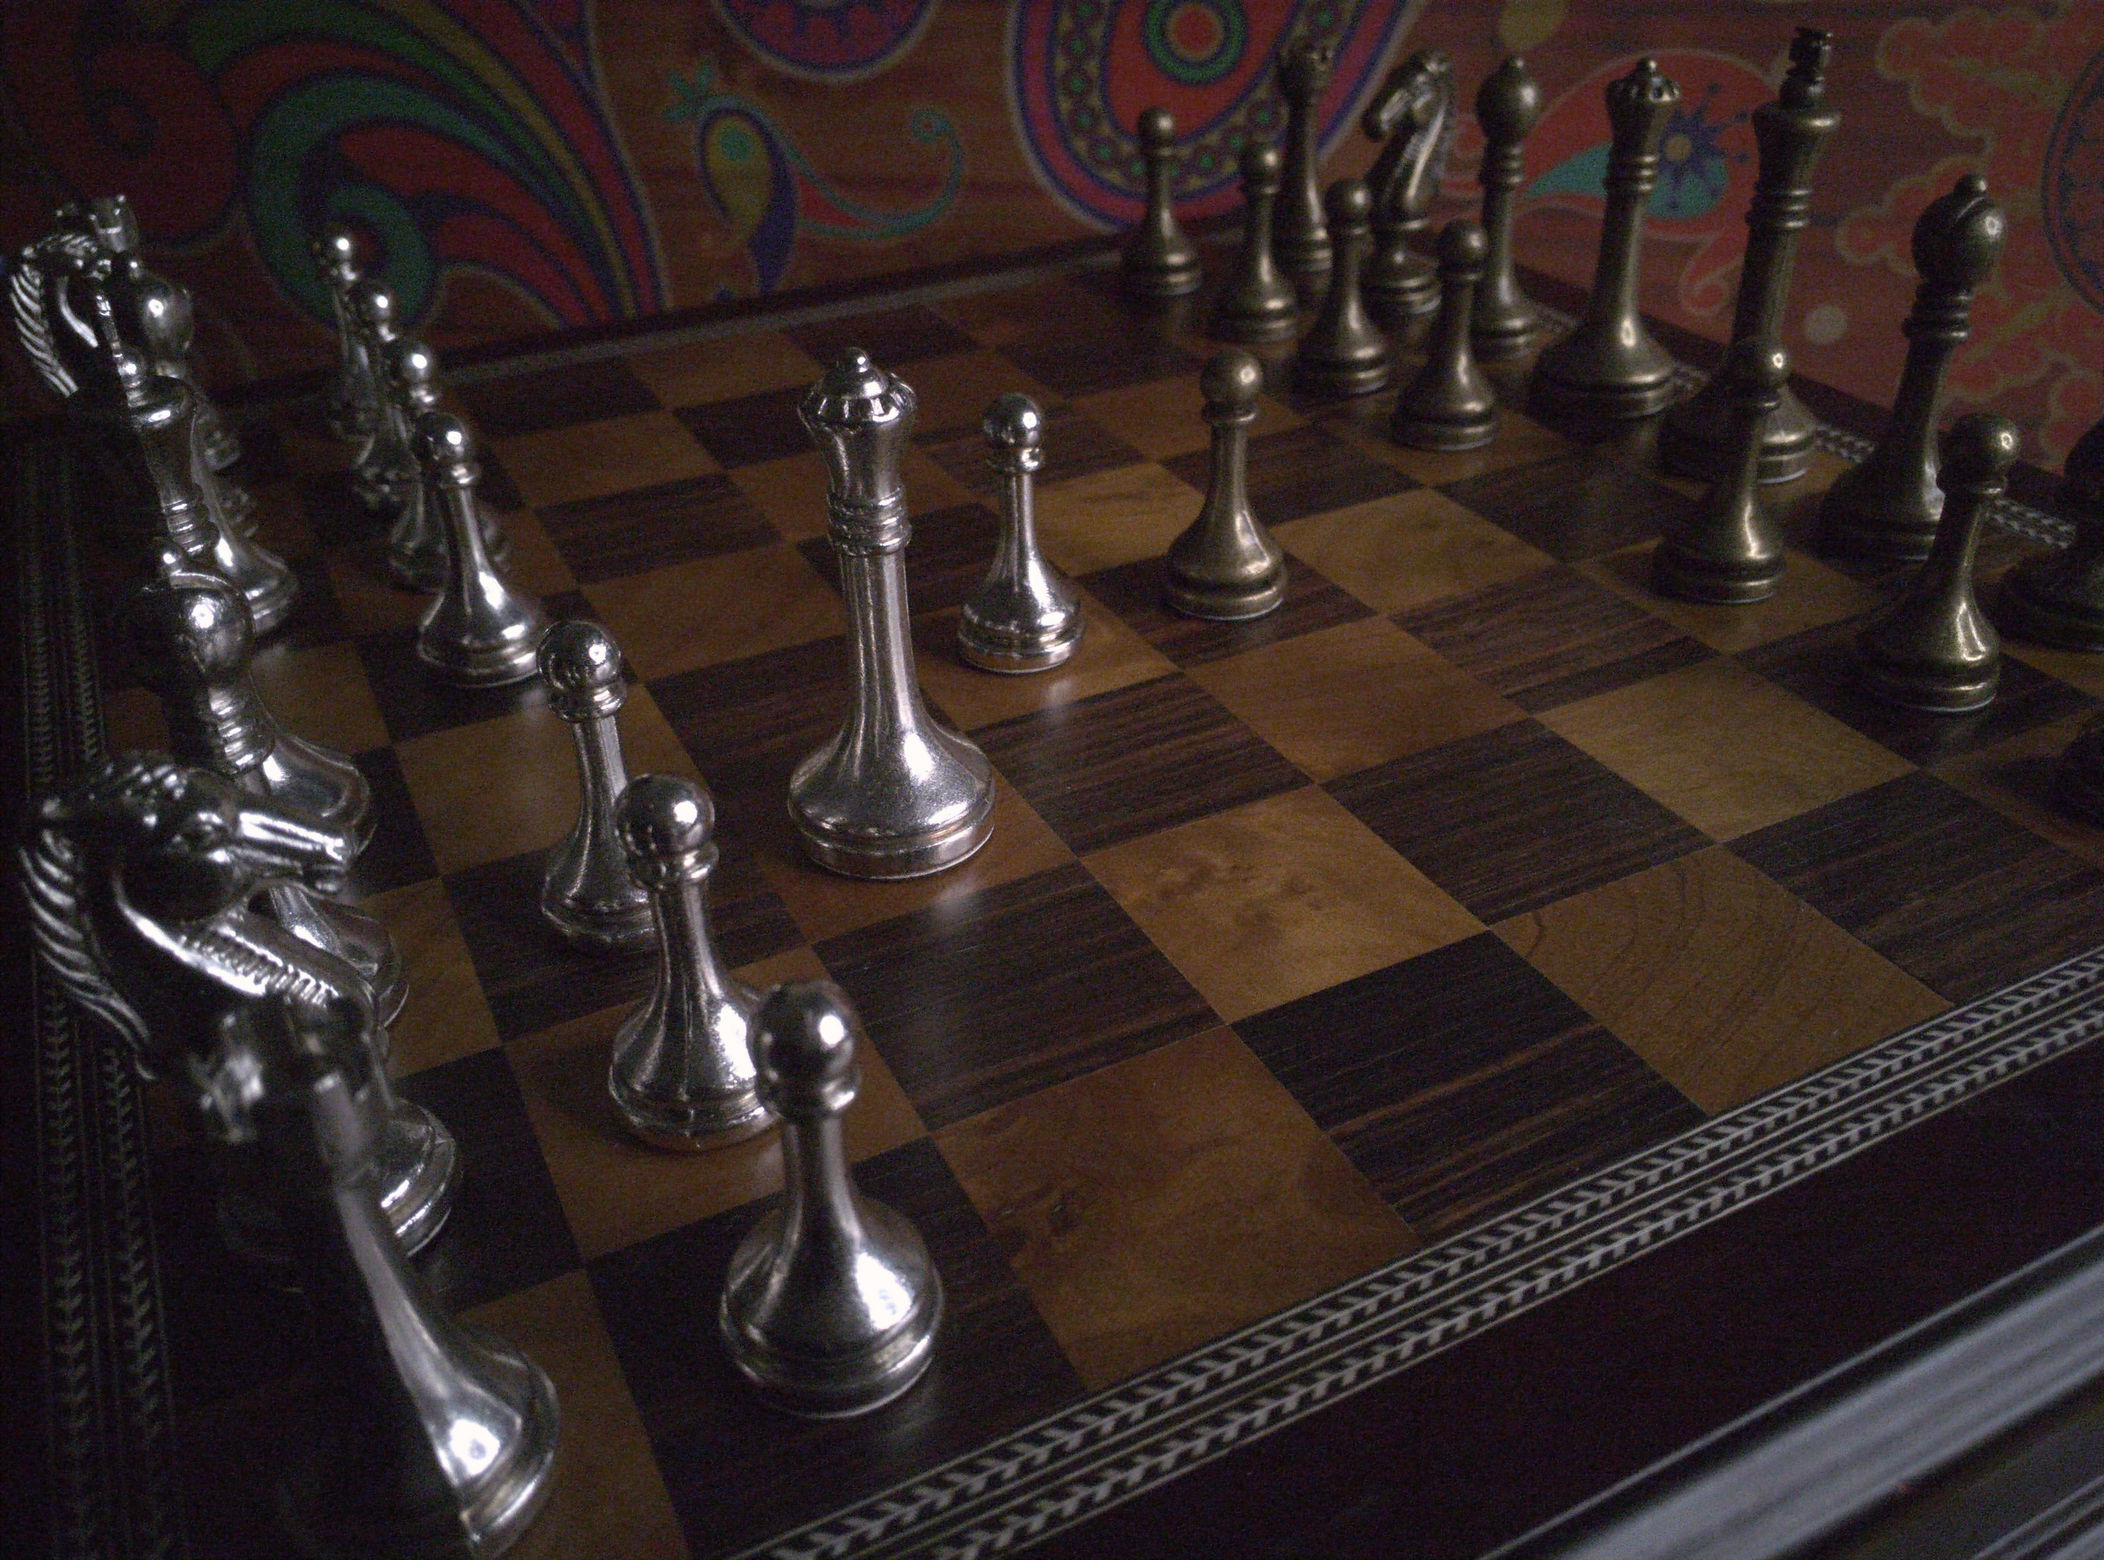
\includegraphics[width=\linewidth]{img/presentazione/dncnn/scacchi_denoise_dncnn.png}\\[0.3em]
            PSNR=31.1354
        \end{minipage} \\[1em]
        % Seconda riga: GT, Autoencoder, BM3D
        \begin{minipage}{0.28\linewidth}
            \centering
            \textbf{GT}\\[0.3em]
            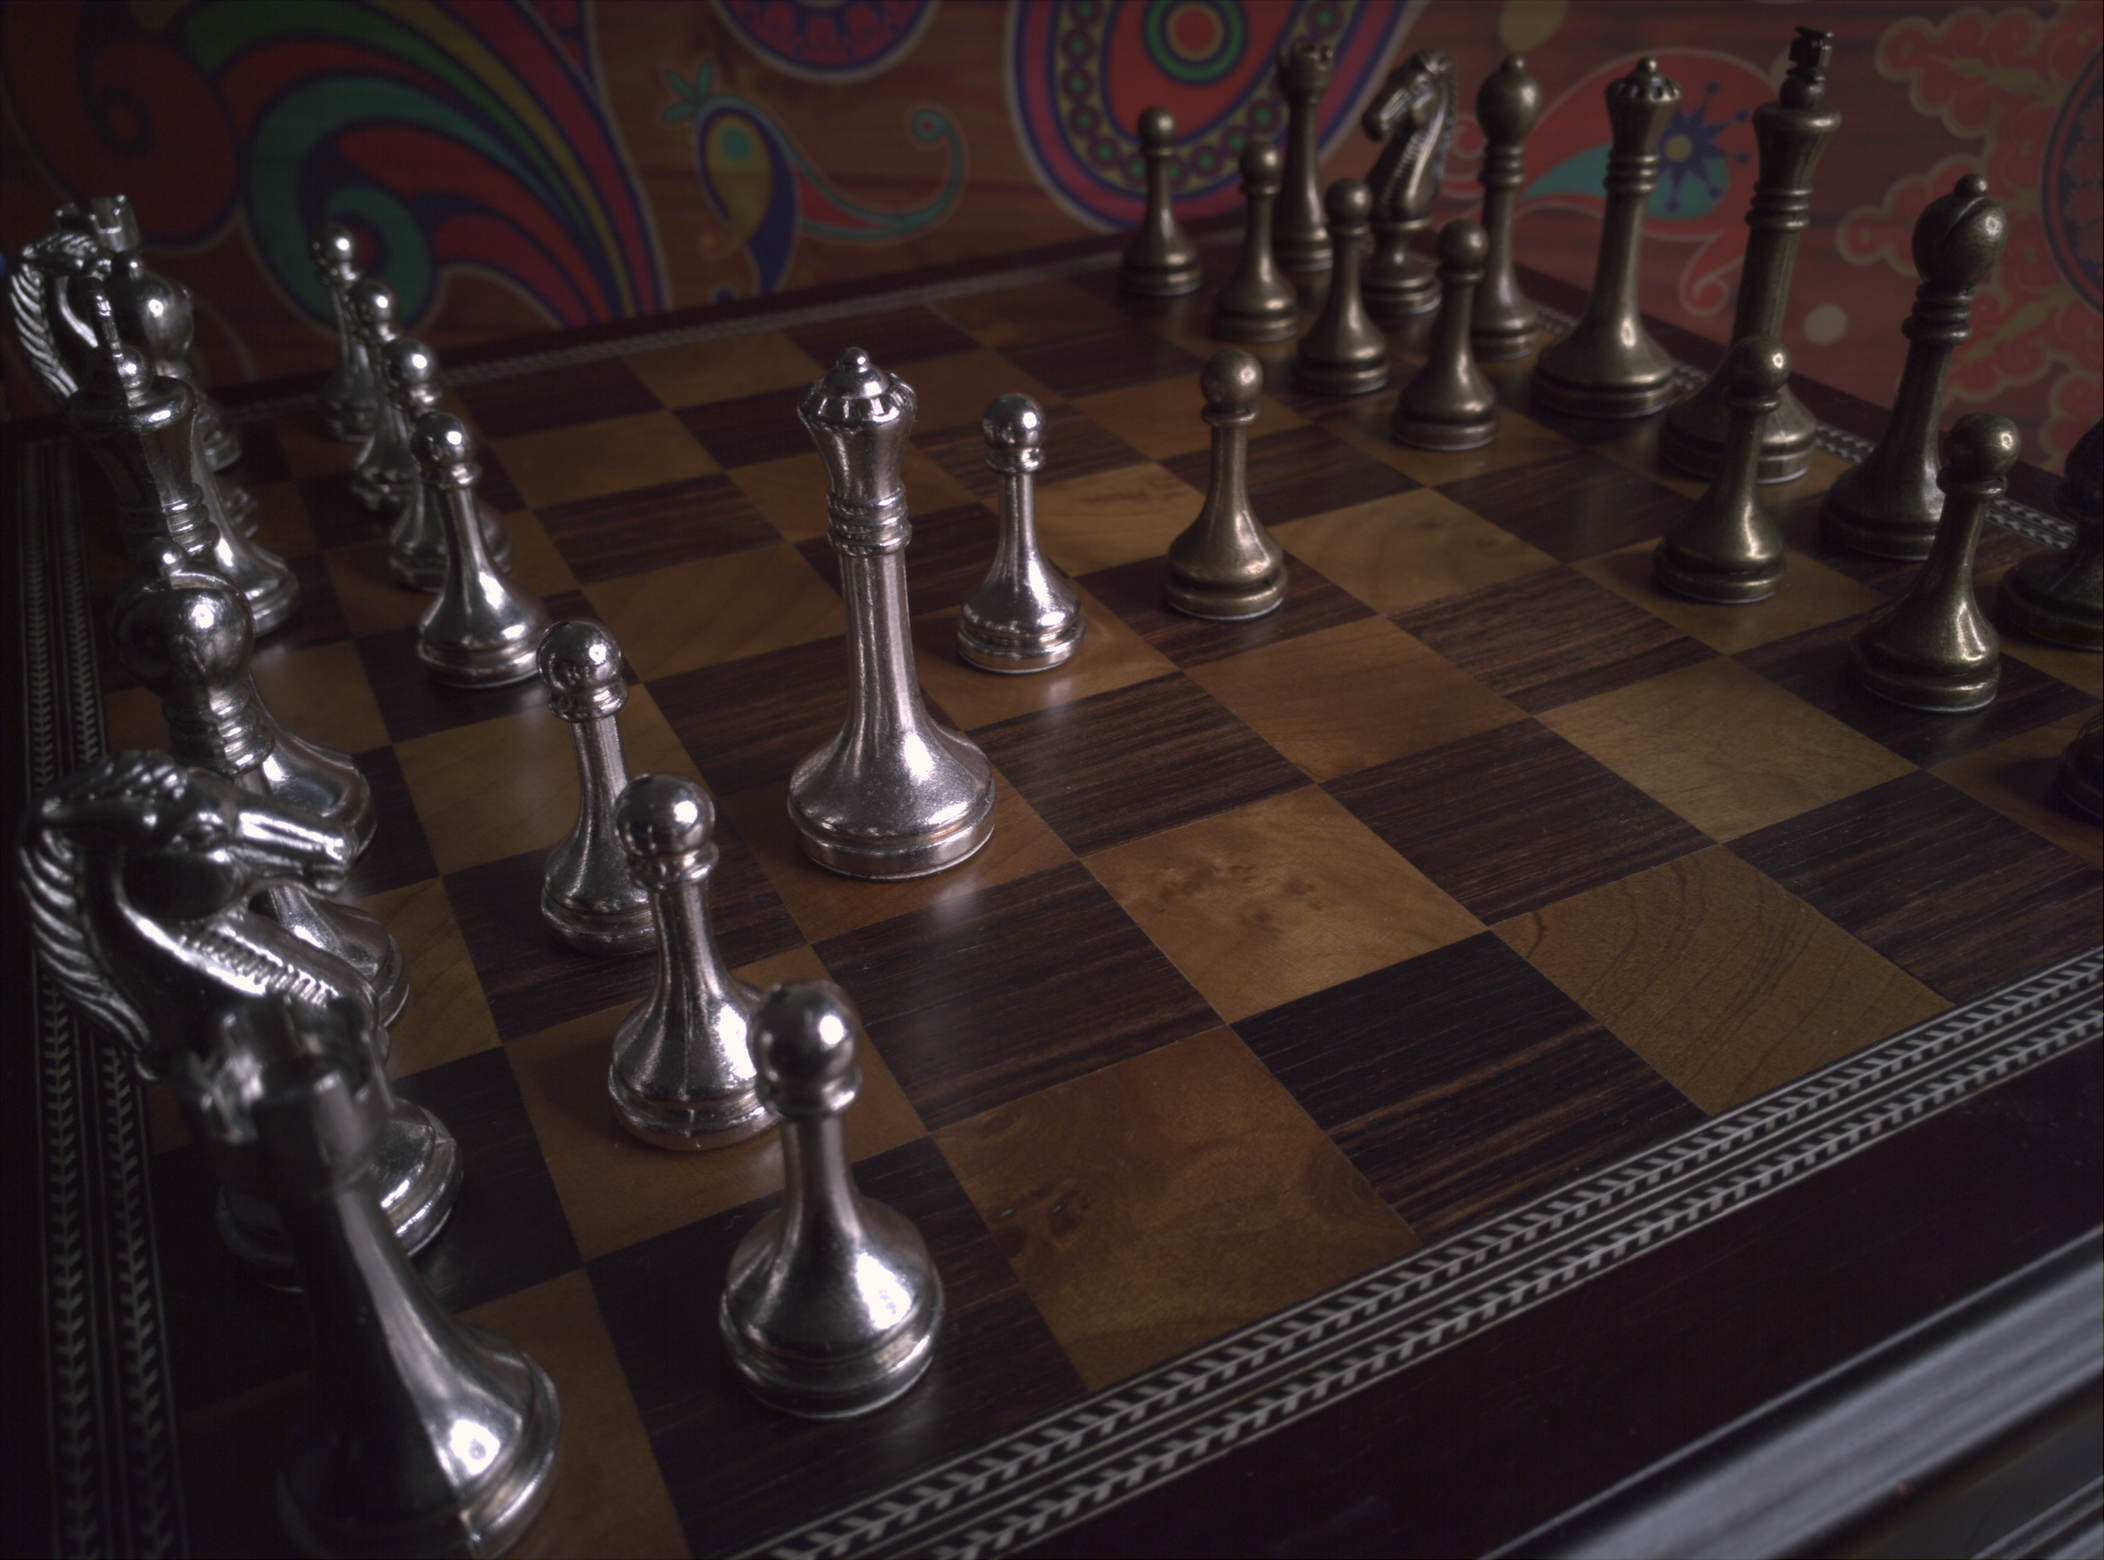
\includegraphics[width=\linewidth]{img/presentazione/sidd_scacchi_gt.PNG}\\[0.3em]
            --
        \end{minipage} &
        \begin{minipage}{0.28\linewidth}
            \centering
            \textbf{Autoencoder}\\[0.3em]
            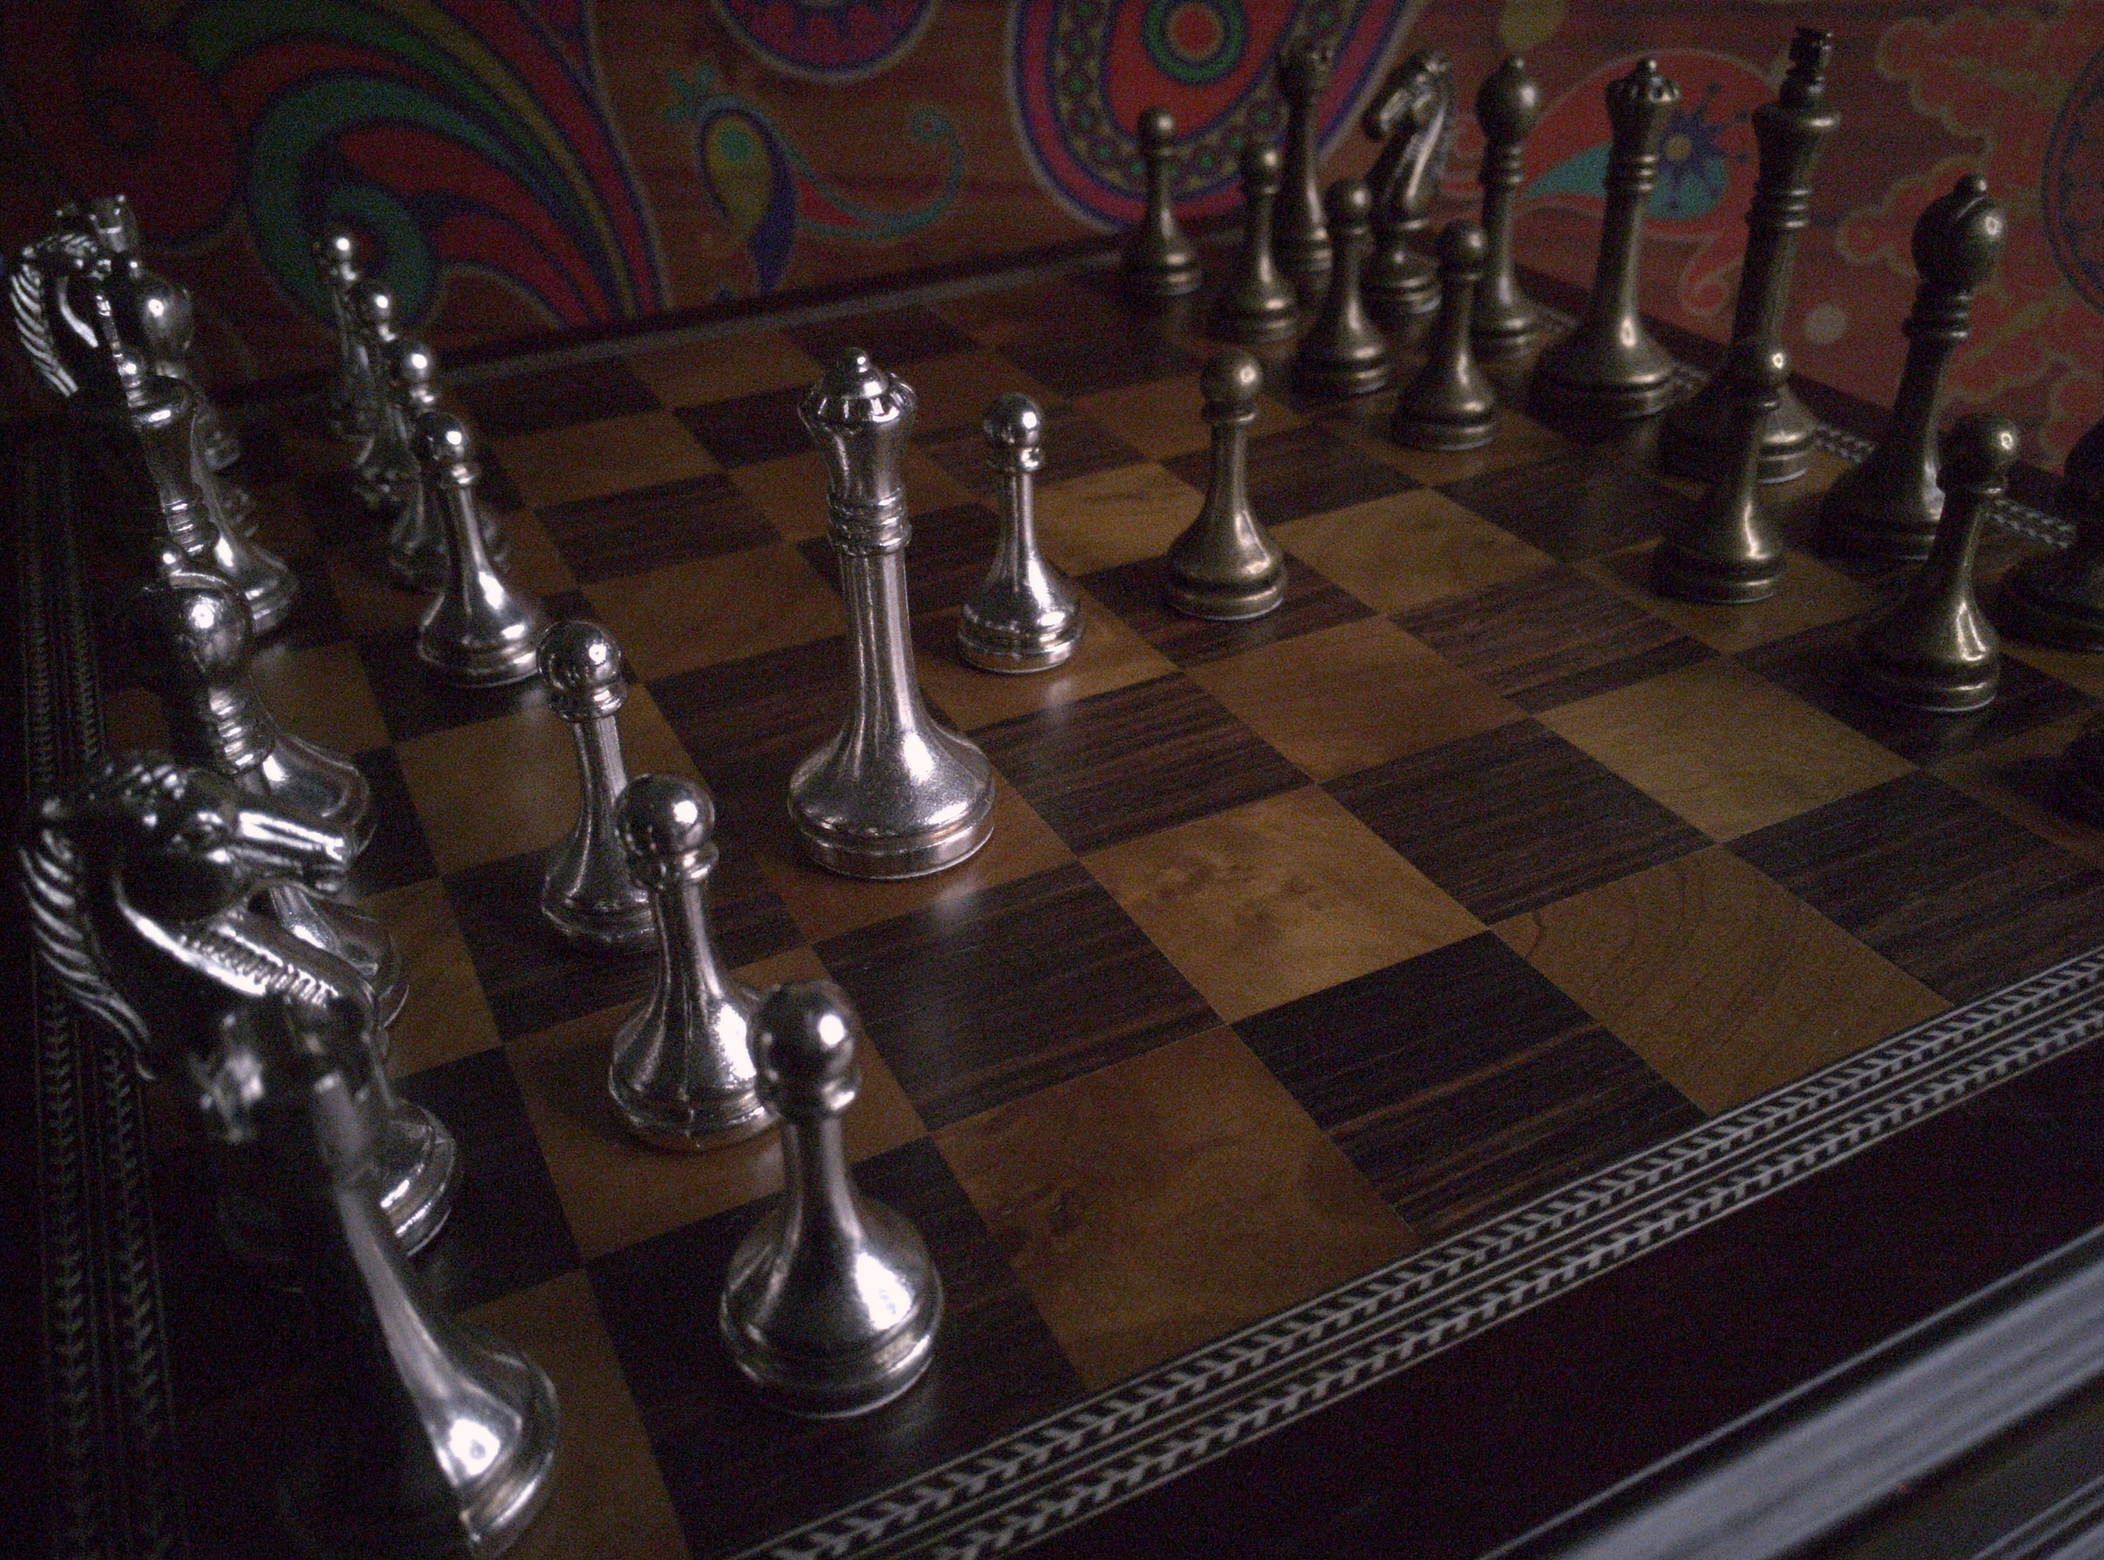
\includegraphics[width=\linewidth]{img/presentazione/autoen/scacchi_denoise_autoen.png}\\[0.3em]
            PSNR=29.8578
        \end{minipage} &
        \begin{minipage}{0.28\linewidth}
            \centering
            \textbf{BM3D}\\[0.3em]
            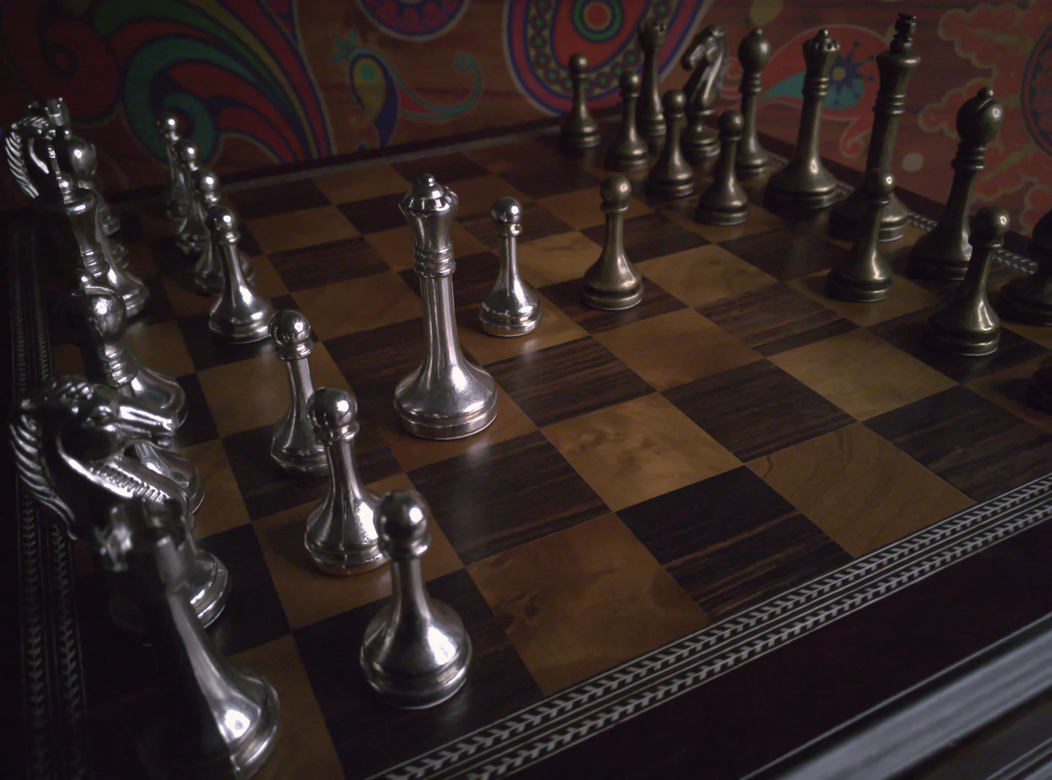
\includegraphics[width=\linewidth]{img/presentazione/bm3d/scacchi_denoise_bm3d_2.png}\\[0.3em]
            PSNR=34.1982
        \end{minipage} \\
    \end{tabular}
\end{frame}

\begin{frame}
  \frametitle{Risultati training modelli}
  \begin{itemize}
    \item Si è notato come Ridnet abbia valori e risultati migliori rispetto agli altri 2 modelli
    \item BM3D risulta meno efficace in caso di elevato rumore a differenza di Ridnet e DnCNN
  \end{itemize}
  

\end{frame}


\begin{frame}{Risultati di training}
  \begin{itemize}
    \item \textbf{RidNet} è il modello più robusto:
      \begin{itemize}
        \item Prestazioni migliori o comparabili in tutti i dataset.
        \item Mantiene valori alti anche con rumore elevato ($\sigma=50$: 26–29 dB).
      \end{itemize}
    \item \textbf{DnCNN} ha risultati intermedi:
      \begin{itemize}
        \item Tipicamente 2–4 dB sotto RidNet.
        \item Calo più evidente con rumore elevato.
      \end{itemize}
    \item \textbf{Autoencoder} è il meno performante:
      \begin{itemize}
        \item Gap medio di 5–7 dB rispetto a RidNet.
        \item Prestazioni limitate su tutti i dataset.
      \end{itemize}
    \item \textbf{BM3D} rimane competitivo a basso rumore:
      \begin{itemize}
        \item $\sigma=15$: risultati vicini a DnCNN.
        \item Degrada più rapidamente quando $\sigma$ cresce
      \end{itemize}
    \item Caso particolare: \textbf{scacchi}
      \begin{itemize}
        \item A $\sigma \approx 16$, BM3D (34.2 dB) e RidNet (34.4 dB) offrono le migliori prestazioni.
      \end{itemize}
  \end{itemize}
\end{frame}






%%%%%%%%%%%%%%%%%% FINETUNE  %%%%%%%%%%%%%%%%%%%%%%%%%%%%%%%%%%%%%%%%%%%%%%%%%%%%%%%%%%%%%%%%%%

\begin{frame}{Fine tuning}
  \begin{itemize}
    \item Fine tuning sul dataset Kvasir per specializzazione su immagini mediche
  \end{itemize}

%\begin{tabular*}{width}{cols}
    
%\end{tabular*}


    \begin{tabular*}{\textwidth}{c@{\hspace{0.2em}}c@{\hspace{0.2em}}c@{\hspace{0.2em}}c}

        \small{\textbf{Accuracy}} &

        \begin{minipage}{0.28\linewidth}
            \centering
            \textbf{Ridnet}\\[0.3em]
            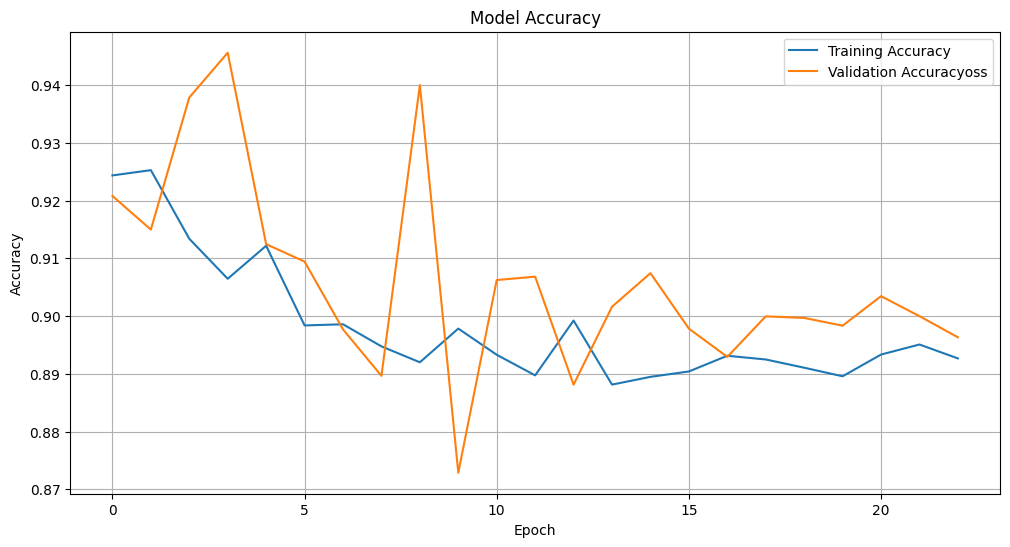
\includegraphics[width=\linewidth]{img/finetune/ridnet/ridnet_finetune_accuracy.png}\\[0.3em]

        \end{minipage} &

        \begin{minipage}{0.28\linewidth}
            \centering
            \textbf{DnCNN}\\[0.3em]
            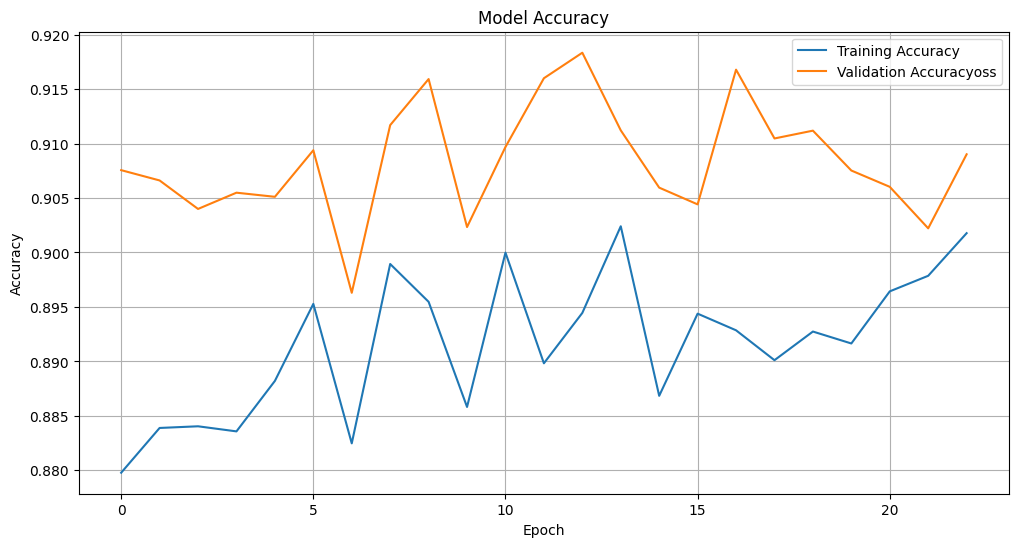
\includegraphics[width=\linewidth]{img/finetune/dncnn/dncnn_finetune_accurcy.png}\\[0.3em]
        \end{minipage} &

        \begin{minipage}{0.28\linewidth}
            \centering
            \textbf{Autoencoder}\\[0.3em]
            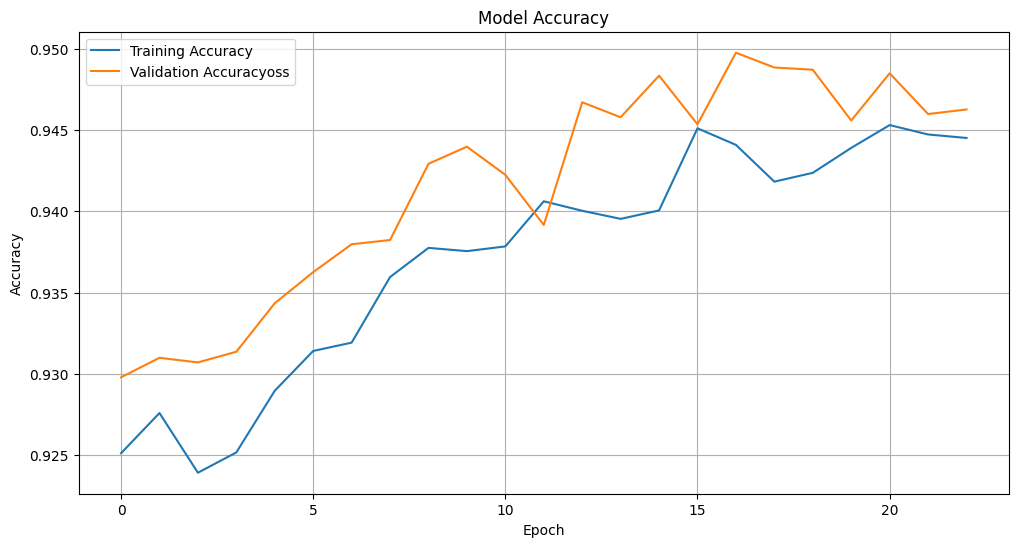
\includegraphics[width=\linewidth]{img/finetune/autoencoder/autoen_finetune_accurcy.png}\\[0.3em]
        \end{minipage} \\

        \small{\textbf{Loss}} &

        \begin{minipage}{0.28\linewidth}
            \centering
            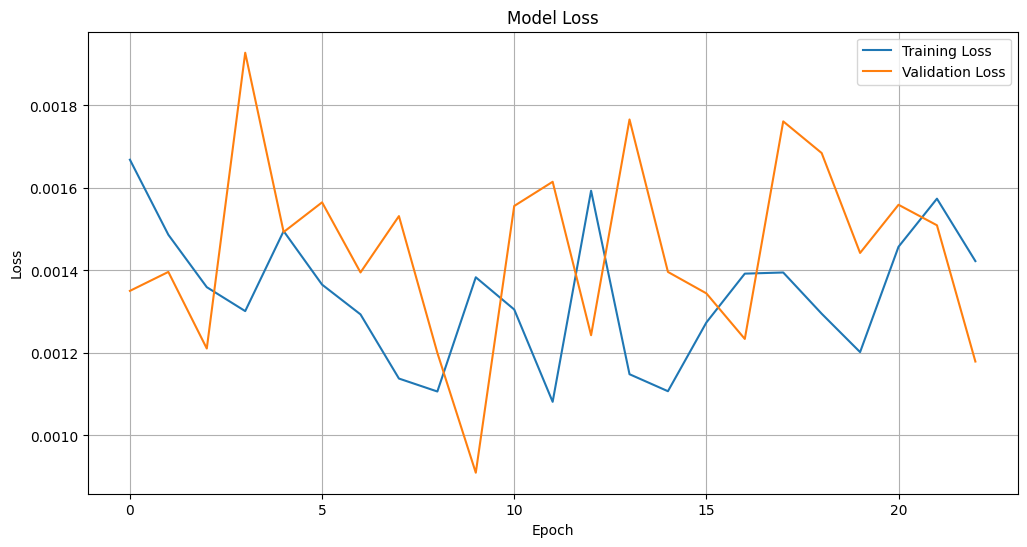
\includegraphics[width=\linewidth]{img/finetune/ridnet/ridnet_finetune_loss.png}\\[0.3em]
        \end{minipage} &

        \begin{minipage}{0.28\linewidth}
            \centering
            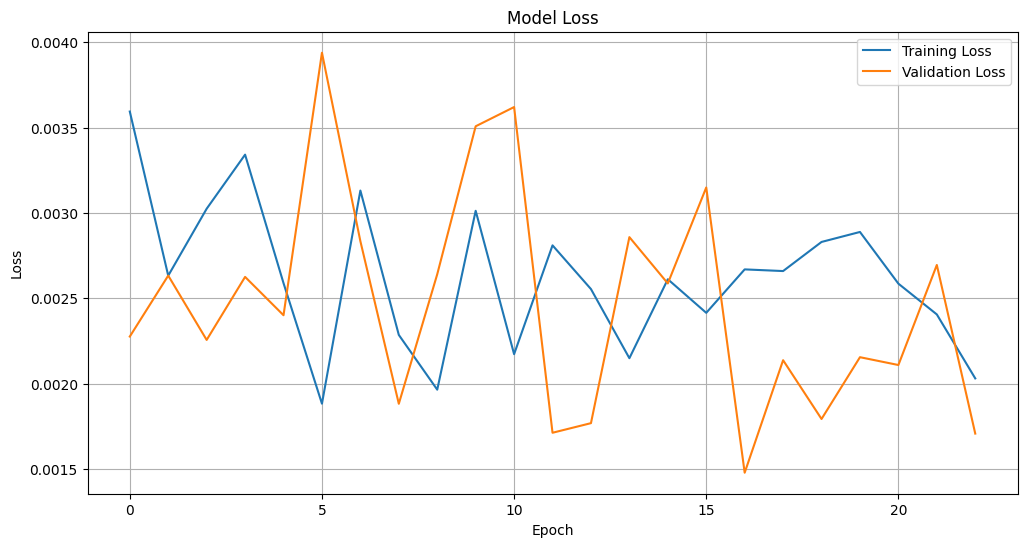
\includegraphics[width=\linewidth]{img/finetune/dncnn/dncnn_finetune_loss.png}\\[0.3em]
        \end{minipage} &

        \begin{minipage}{0.28\linewidth}
            \centering
            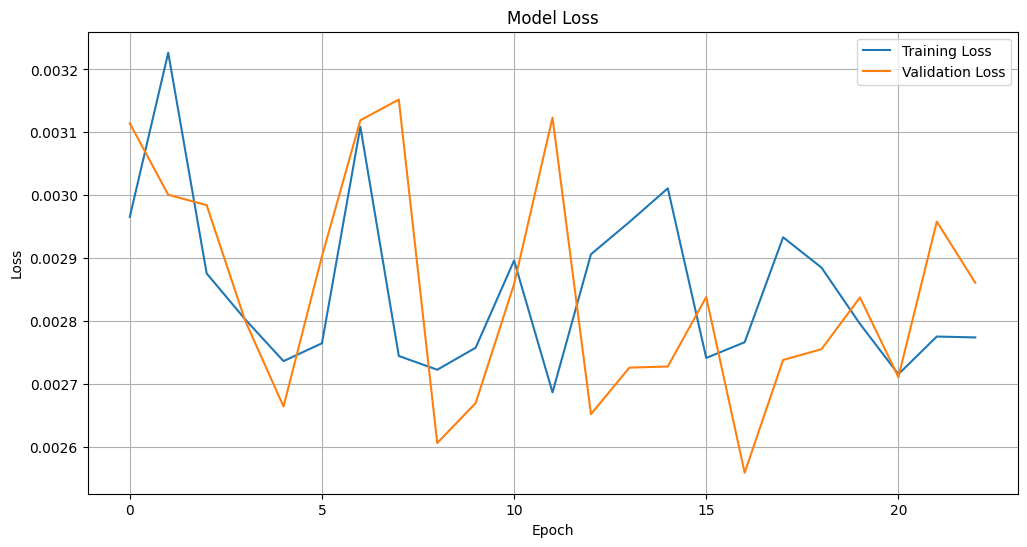
\includegraphics[width=\linewidth]{img/finetune/autoencoder/autoen_finetune_loss.png}\\[0.3em]
        \end{minipage} \\
    \end{tabular*}

\end{frame}

% --- Denoising σ=15 ---
\begin{frame}{Pre Fine Tuning $\sigma=15$}
    \centering
    \renewcommand{\arraystretch}{1.5}
    \begin{tabular}{c c c}
        \begin{minipage}{0.28\linewidth}
            \centering
            \textbf{Noisy}\\[0.3em]
            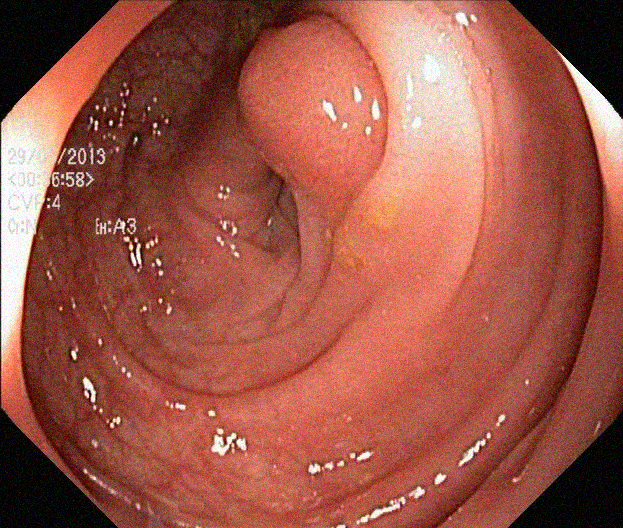
\includegraphics[width=\linewidth]{img/presentazione/noisy/kvasir_noise_15.png}\\[0.3em]
            $\sigma=15$
        \end{minipage} &
        \begin{minipage}{0.28\linewidth}
            \centering
            \textbf{RidNet}\\[0.3em]
            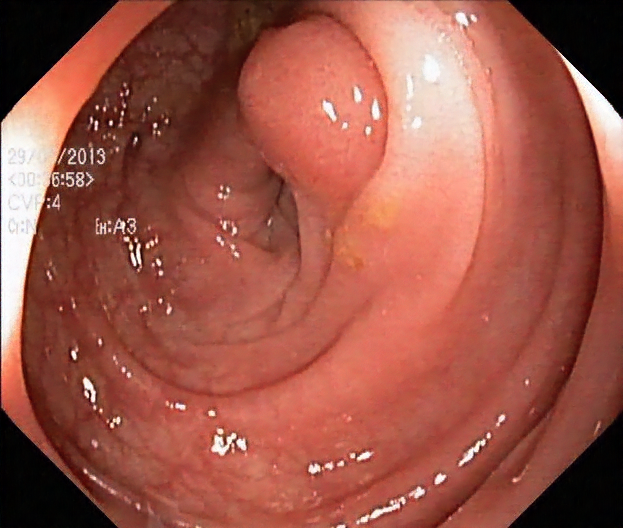
\includegraphics[width=\linewidth]{img/presentazione/ridnet/kvasir_denoise_ridnet_pre_15.png}\\[0.3em]
            PSNR=35.3678
        \end{minipage} &
        \begin{minipage}{0.28\linewidth}
            \centering
            \textbf{DnCNN}\\[0.3em]
            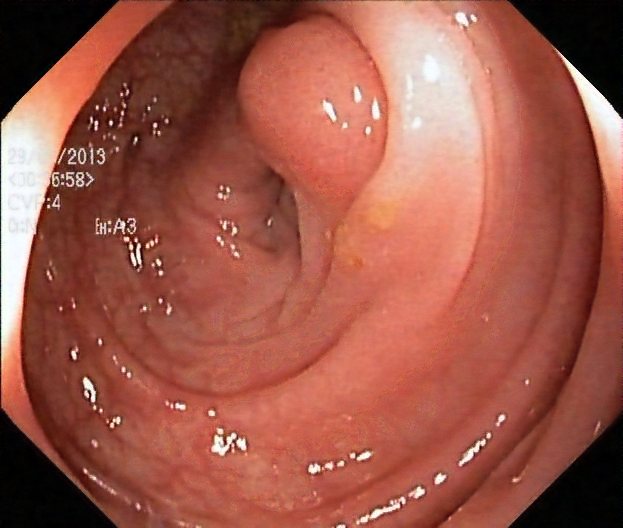
\includegraphics[width=\linewidth]{img/presentazione/dncnn/kvasir_denoise_dncnn_pre_15.png}\\[0.3em]
            PSNR=33.2413
        \end{minipage} \\[1em]
        \begin{minipage}{0.28\linewidth}
            \centering
            \textbf{GT}\\[0.3em]
            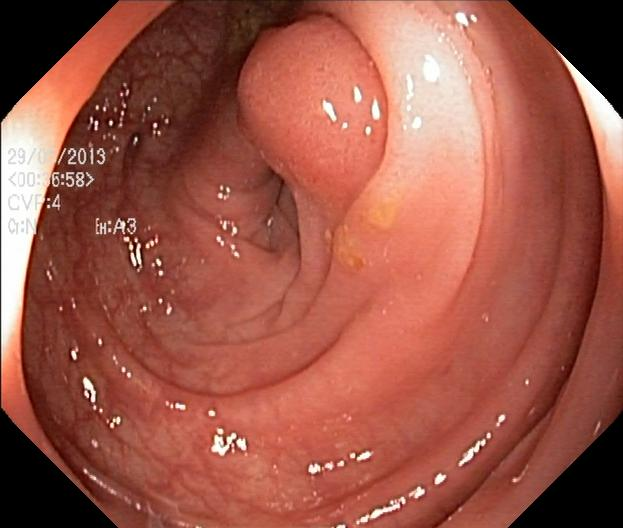
\includegraphics[width=\linewidth]{img/presentazione/kvasir.jpg}\\[0.3em]
            --
        \end{minipage} &
        \begin{minipage}{0.28\linewidth}
            \centering
            \textbf{Autoencoder}\\[0.3em]
            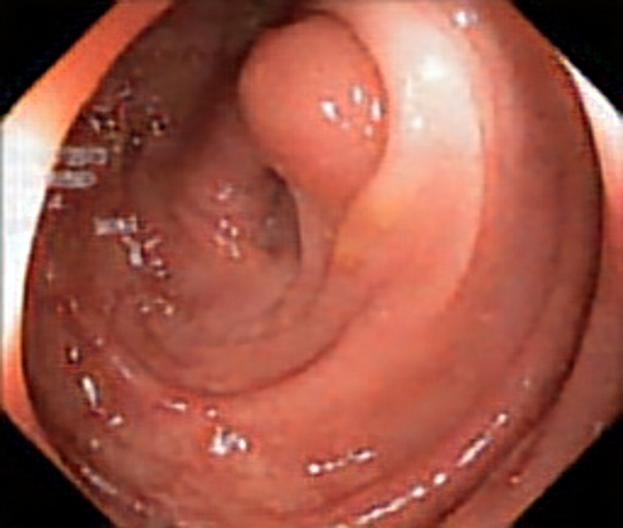
\includegraphics[width=\linewidth]{img/presentazione/autoen/kvasir_denoise_autoen_pre_15.png}\\[0.3em]
            PSNR=28.1402
        \end{minipage} &
        \begin{minipage}{0.28\linewidth}
            \centering
            \textbf{BM3D}\\[0.3em]
            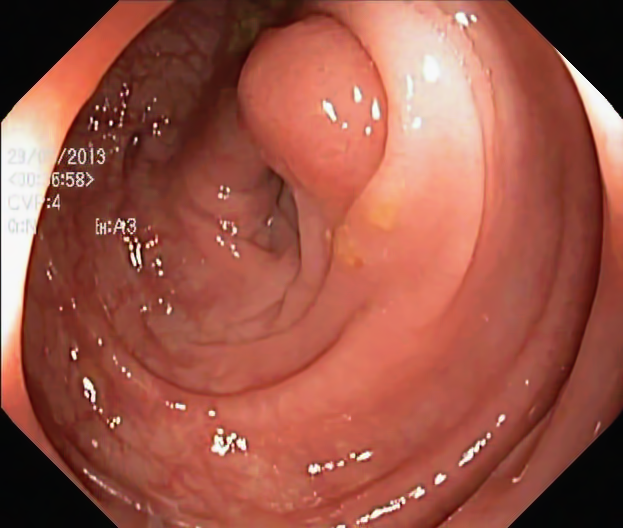
\includegraphics[width=\linewidth]{img/presentazione/bm3d/kvasir_denoise_bm3d_15.png}\\[0.3em]
            PSNR=35.0775
        \end{minipage} \\
    \end{tabular}
\end{frame}



\begin{frame}{Pre Fine Tuning $\sigma=25$}
    \centering
    \renewcommand{\arraystretch}{1.5}
    \begin{tabular}{c c c}
        \begin{minipage}{0.28\linewidth}
            \centering
            \textbf{Noisy}\\[0.3em]
            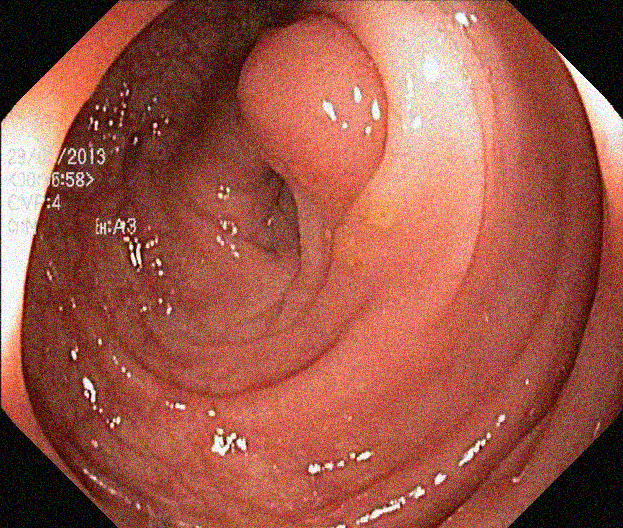
\includegraphics[width=\linewidth]{img/presentazione/noisy/kvasir_noise_25.png}\\[0.3em]
            $\sigma=25$
        \end{minipage} &
        \begin{minipage}{0.28\linewidth}
            \centering
            \textbf{RidNet}\\[0.3em]
            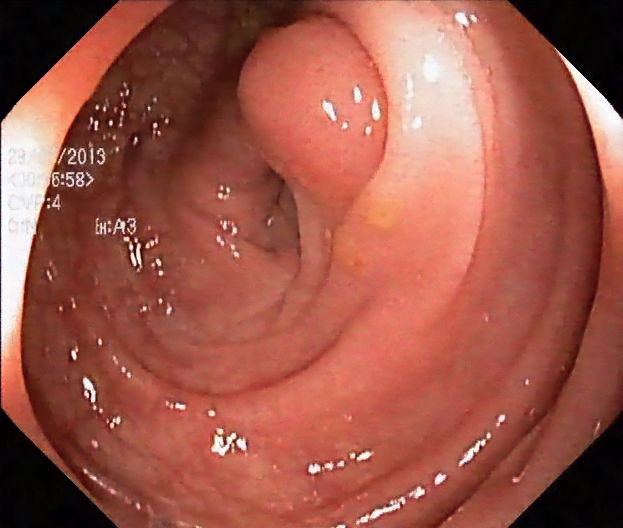
\includegraphics[width=\linewidth]{img/presentazione/ridnet/kvasir_denoise_ridnet_pre_25.png}\\[0.3em]
            PSNR=32.9191
        \end{minipage} &
        \begin{minipage}{0.28\linewidth}
            \centering
            \textbf{DnCNN}\\[0.3em]
            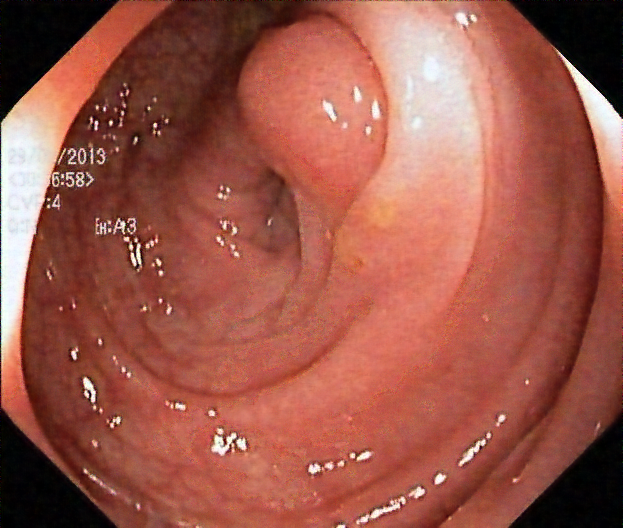
\includegraphics[width=\linewidth]{img/presentazione/dncnn/kvasir_denoise_dncnn_pre_25.png}\\[0.3em]
            PSNR=30.6794
        \end{minipage} \\[1em]
        \begin{minipage}{0.28\linewidth}
            \centering
            \textbf{GT}\\[0.3em]
            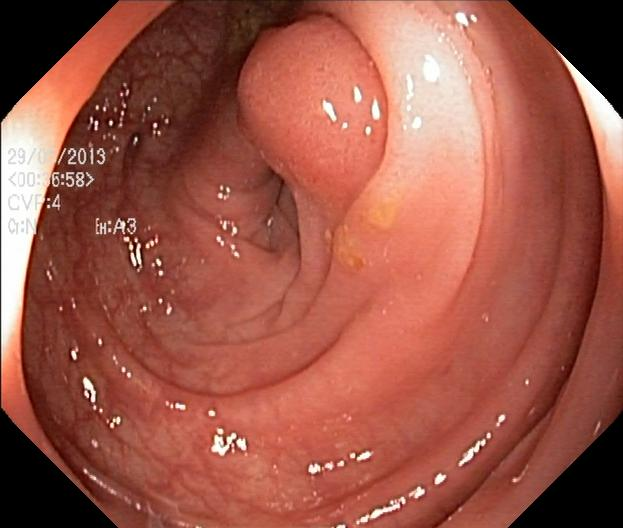
\includegraphics[width=\linewidth]{img/presentazione/kvasir.jpg}\\[0.3em]
            --
        \end{minipage} &
        \begin{minipage}{0.28\linewidth}
            \centering
            \textbf{Autoencoder}\\[0.3em]
            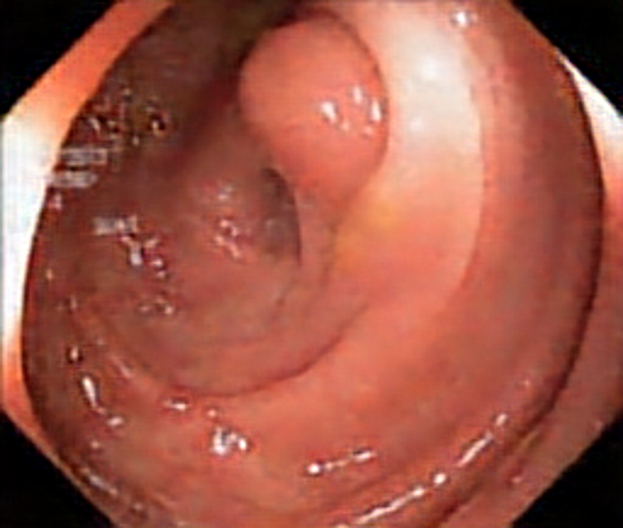
\includegraphics[width=\linewidth]{img/presentazione/autoen/kvasir_denoise_autoen_pre_25.png}\\[0.3em]
            PSNR=27.4472
        \end{minipage} &
        \begin{minipage}{0.28\linewidth}
            \centering
            \textbf{BM3D}\\[0.3em]
            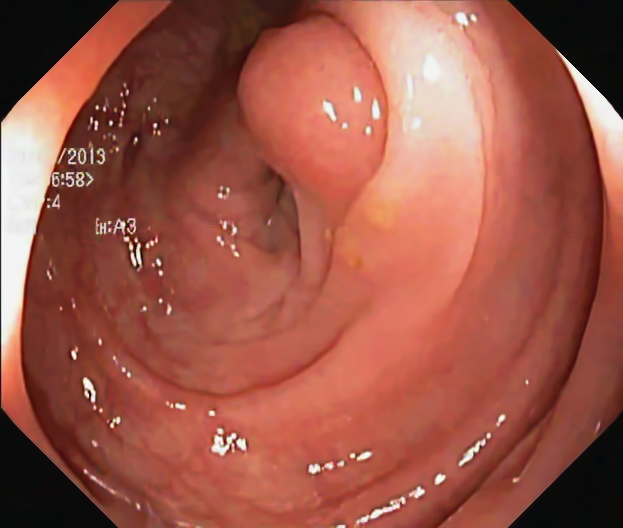
\includegraphics[width=\linewidth]{img/presentazione/bm3d/kvasir_denoise_bm3d_25.png}\\[0.3em]
            PSNR=32.1350
        \end{minipage} \\
    \end{tabular}
\end{frame}

% --- Denoising σ=15 ---
\begin{frame}{Pre Fine Tuning $\sigma=50$}
    \centering
    \renewcommand{\arraystretch}{1.5}
    \begin{tabular}{c c c}
        \begin{minipage}{0.28\linewidth}
            \centering
            \textbf{Noisy}\\[0.3em]
            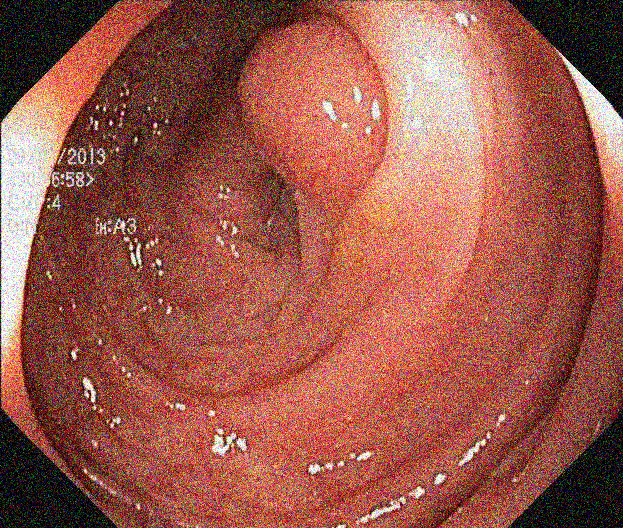
\includegraphics[width=\linewidth]{img/presentazione/noisy/kvasir_noise_50.png}\\[0.3em]
            $\sigma=50$
        \end{minipage} &
        \begin{minipage}{0.28\linewidth}
            \centering
            \textbf{RidNet}\\[0.3em]
            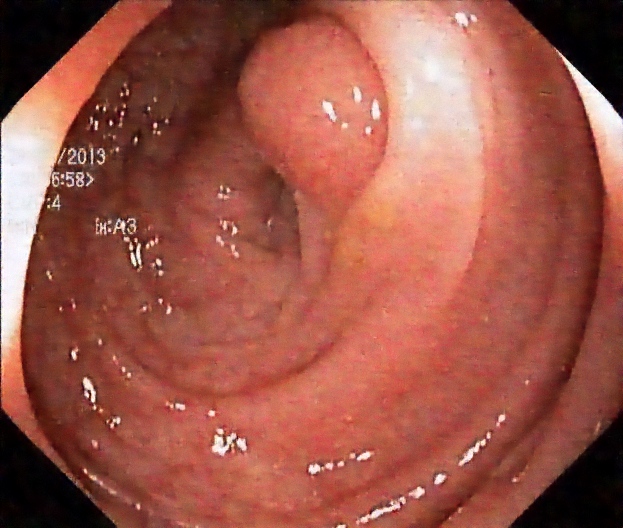
\includegraphics[width=\linewidth]{img/presentazione/ridnet/kvasir_denoise_ridnet_pre_50.png}\\[0.3em]
            PSNR=29.4796
        \end{minipage} &
        \begin{minipage}{0.28\linewidth}
            \centering
            \textbf{DnCNN}\\[0.3em]
            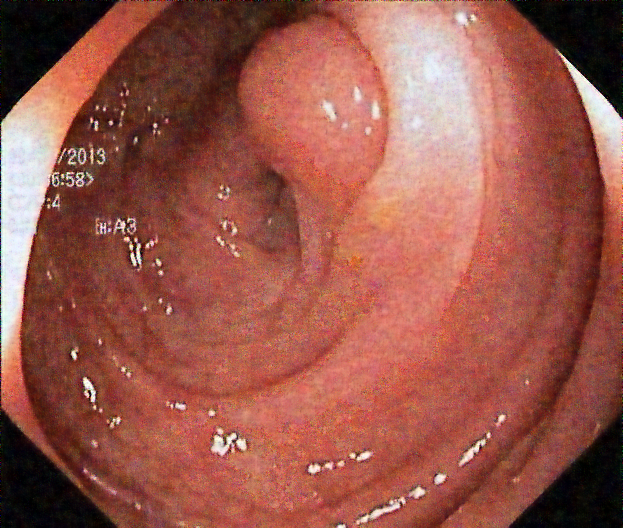
\includegraphics[width=\linewidth]{img/presentazione/dncnn/kvasir_denoise_dncnn_pre_50.png}\\[0.3em]
            PSNR=25.9305
        \end{minipage} \\[1em]
        \begin{minipage}{0.28\linewidth}
            \centering
            \textbf{GT}\\[0.3em]
            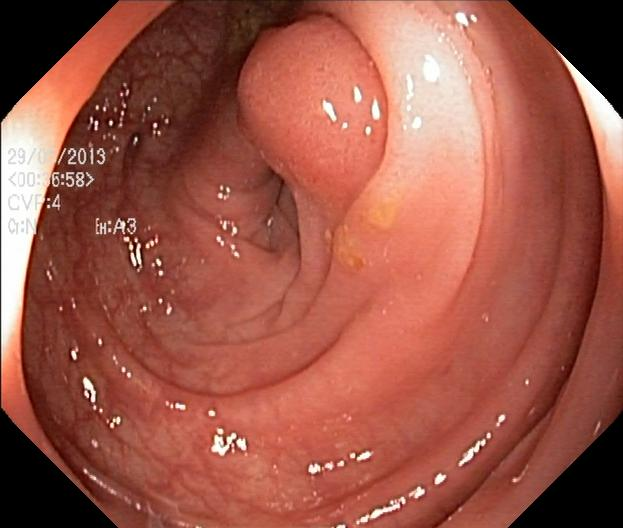
\includegraphics[width=\linewidth]{img/presentazione/kvasir.jpg}\\[0.3em]
            --
        \end{minipage} &
        \begin{minipage}{0.28\linewidth}
            \centering
            \textbf{Autoencoder}\\[0.3em]
            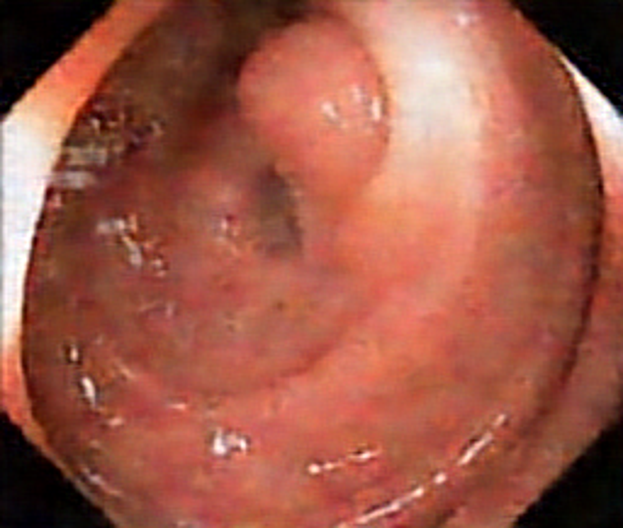
\includegraphics[width=\linewidth]{img/presentazione/autoen/kvasir_denoise_autoen_pre_50.png}\\[0.3em]
            PSNR=25.8299
        \end{minipage} &
        \begin{minipage}{0.28\linewidth}
            \centering
            \textbf{BM3D}\\[0.3em]
            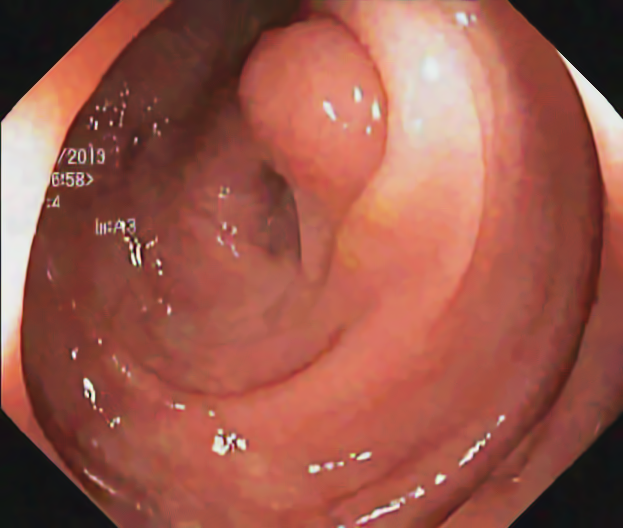
\includegraphics[width=\linewidth]{img/presentazione/bm3d/kvasir_denoise_bm3d_50.png}\\[0.3em]
            PSNR=27.1503
        \end{minipage} \\
    \end{tabular}
\end{frame}




% --- Post Fine Tuning σ=15 ---
\begin{frame}{Post Fine Tuning $\sigma=15$}
    \centering
    \renewcommand{\arraystretch}{1.5}
    \begin{tabular}{c c c}
        % Prima riga: Noisy, RidNet, DnCNN
        \begin{minipage}{0.28\linewidth}
            \centering
            \textbf{Noisy}\\[0.3em]
            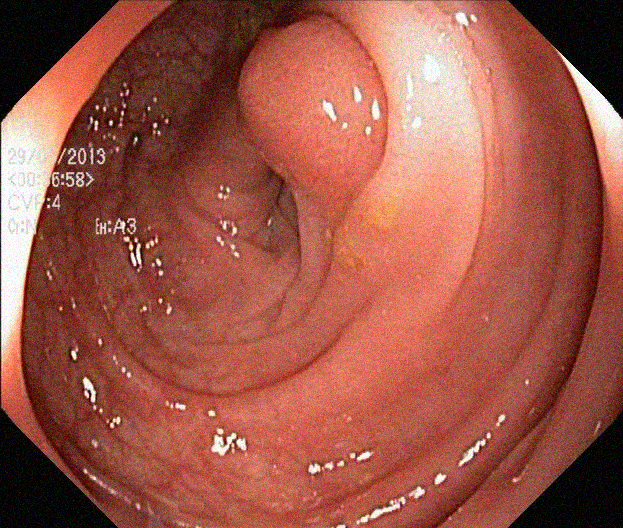
\includegraphics[width=\linewidth]{img/presentazione/noisy/kvasir_noise_15.png}\\[0.3em]
            $\sigma=15$
        \end{minipage} &
        \begin{minipage}{0.28\linewidth}
            \centering
            \textbf{RidNet}\\[0.3em]
            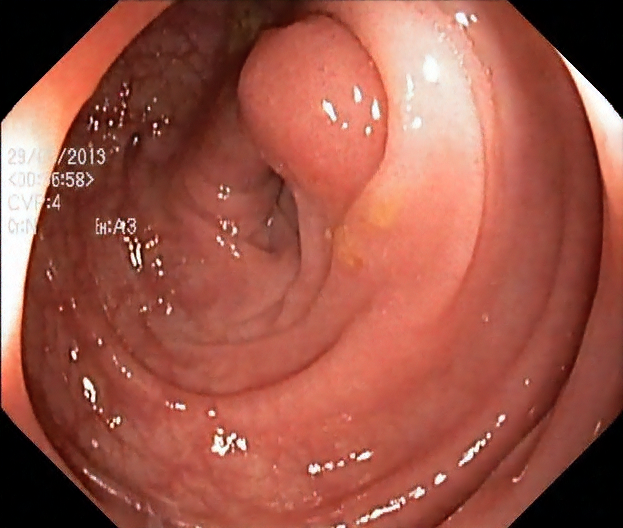
\includegraphics[width=\linewidth]{img/presentazione/ridnet/kvasir_denoise_ridnet_post_15.png}\\[0.3em]
            PSNR=35.7874
        \end{minipage} &
        \begin{minipage}{0.28\linewidth}
            \centering
            \textbf{DnCNN}\\[0.3em]
            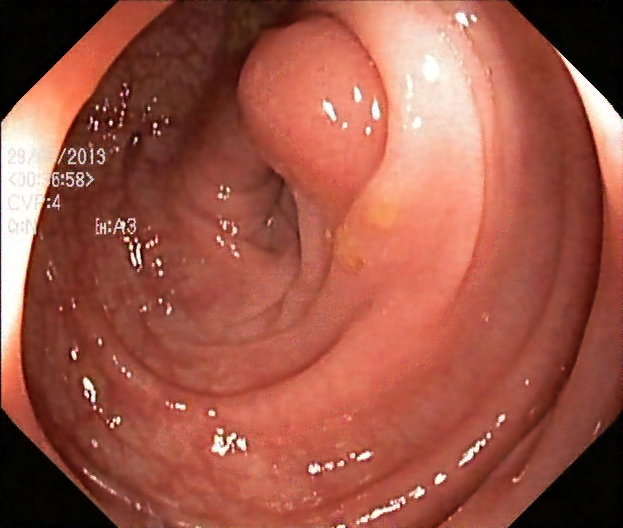
\includegraphics[width=\linewidth]{img/presentazione/dncnn/kvasir_denoise_dncnn_post_15.png}\\[0.3em]
            PSNR=33.7068
        \end{minipage} \\[1em]
        % Seconda riga: GT, Autoencoder
        \begin{minipage}{0.28\linewidth}
            \centering
            \textbf{GT}\\[0.3em]
            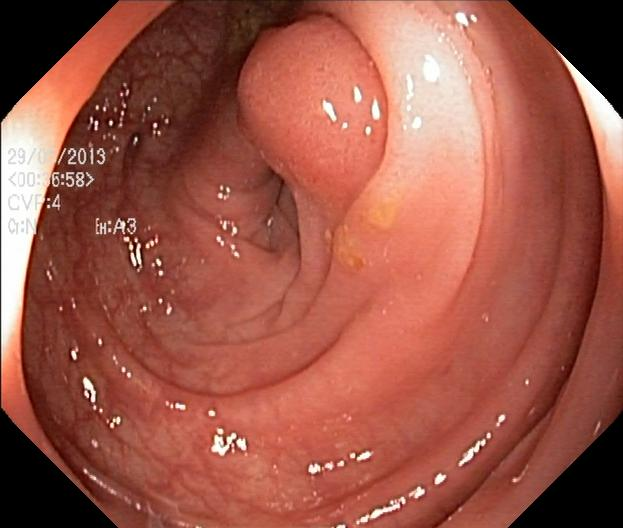
\includegraphics[width=\linewidth]{img/presentazione/kvasir.jpg}\\[0.3em]
            --
        \end{minipage} &
        \begin{minipage}{0.28\linewidth}
            \centering
            \textbf{Autoencoder}\\[0.3em]
            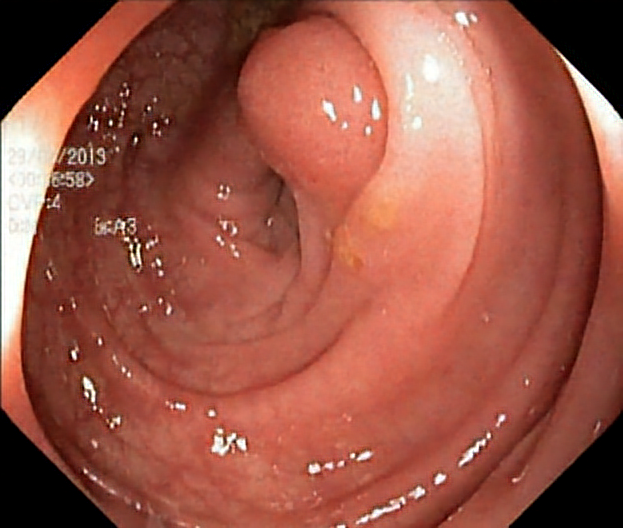
\includegraphics[width=\linewidth]{img/presentazione/autoen/kvasir_denoise_autoen_post_15.png}\\[0.3em]
            PSNR=31.7846
        \end{minipage} &
        \begin{minipage}{0.28\linewidth}
            \centering
            % Cella vuota al posto di BM3D
        \end{minipage} \\
    \end{tabular}
\end{frame}

% --- Post Fine Tuning σ=25 ---
\begin{frame}{Post Fine Tuning $\sigma=25$}
    \centering
    \renewcommand{\arraystretch}{1.5}
    \begin{tabular}{c c c}
        \begin{minipage}{0.28\linewidth}
            \centering
            \textbf{Noisy}\\[0.3em]
            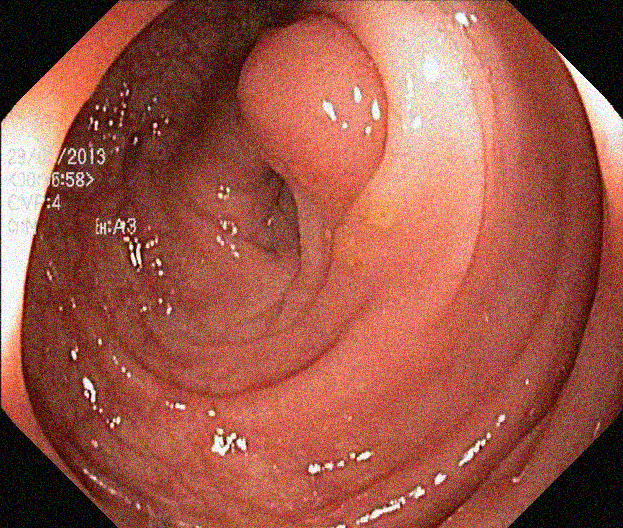
\includegraphics[width=\linewidth]{img/presentazione/noisy/kvasir_noise_25.png}\\[0.3em]
            $\sigma=25$
        \end{minipage} &
        \begin{minipage}{0.28\linewidth}
            \centering
            \textbf{RidNet}\\[0.3em]
            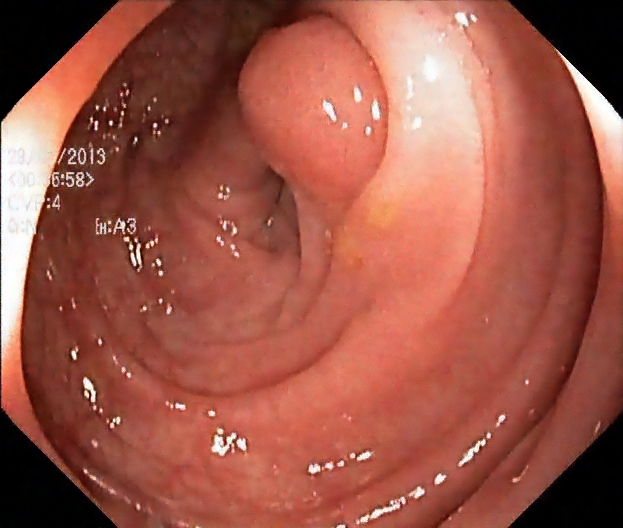
\includegraphics[width=\linewidth]{img/presentazione/ridnet/kvasir_denoise_ridnet_post_25.png}\\[0.3em]
            PSNR=33.4563
        \end{minipage} &
        \begin{minipage}{0.28\linewidth}
            \centering
            \textbf{DnCNN}\\[0.3em]
            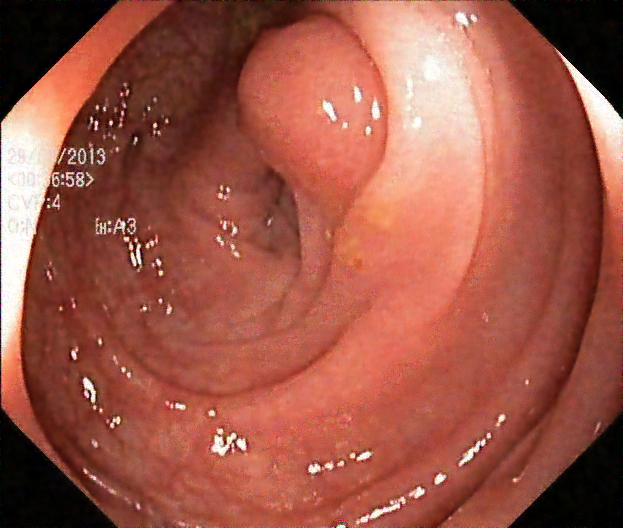
\includegraphics[width=\linewidth]{img/presentazione/dncnn/kvasir_denoise_dncnn_post_25.png}\\[0.3em]
            PSNR=31.3069
        \end{minipage} \\[1em]
        \begin{minipage}{0.28\linewidth}
            \centering
            \textbf{GT}\\[0.3em]
            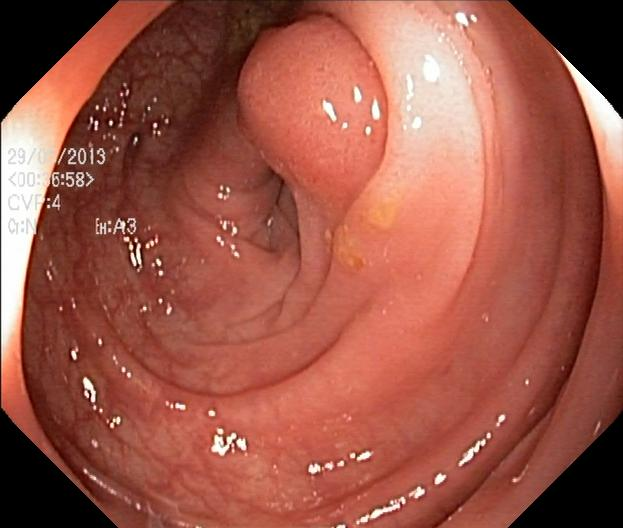
\includegraphics[width=\linewidth]{img/presentazione/kvasir.jpg}\\[0.3em]
            --
        \end{minipage} &
        \begin{minipage}{0.28\linewidth}
            \centering
            \textbf{Autoencoder}\\[0.3em]
            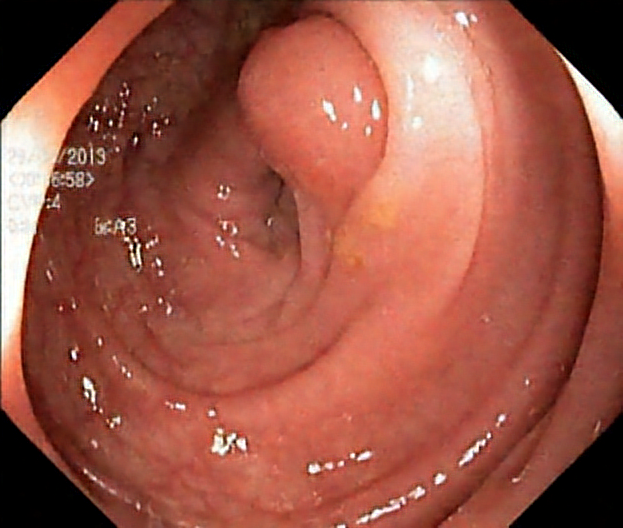
\includegraphics[width=\linewidth]{img/presentazione/autoen/kvasir_denoise_autoen_post_25.png}\\[0.3em]
            PSNR=30.9594
        \end{minipage} &
        \begin{minipage}{0.28\linewidth}
            % Cella vuota
        \end{minipage} \\
    \end{tabular}
\end{frame}

% --- Post Fine Tuning σ=50 ---
\begin{frame}{Post Fine Tuning $\sigma=50$}
    \centering
    \renewcommand{\arraystretch}{1.5}
    \begin{tabular}{c c c}
        \begin{minipage}{0.28\linewidth}
            \centering
            \textbf{Noisy}\\[0.3em]
            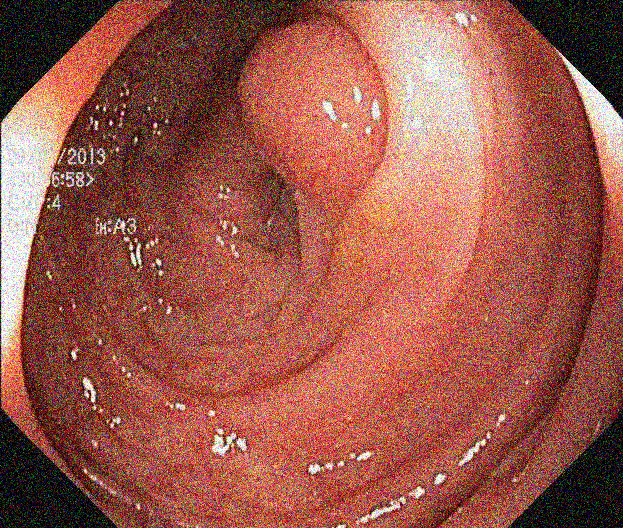
\includegraphics[width=\linewidth]{img/presentazione/noisy/kvasir_noise_50.png}\\[0.3em]
            $\sigma=50$
        \end{minipage} &
        \begin{minipage}{0.28\linewidth}
            \centering
            \textbf{RidNet}\\[0.3em]
            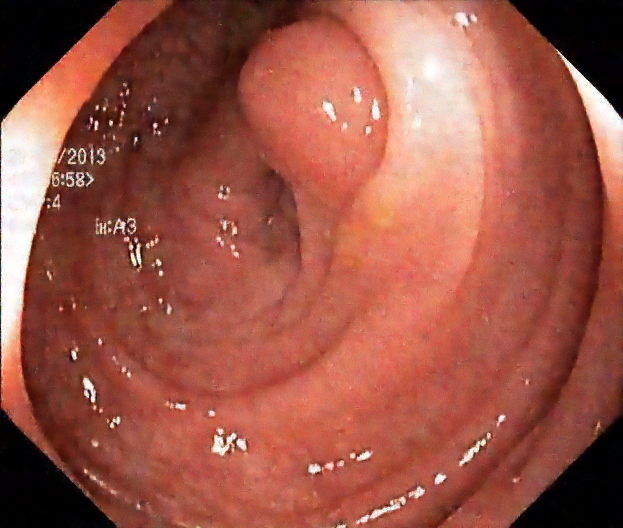
\includegraphics[width=\linewidth]{img/presentazione/ridnet/kvasir_denoise_ridnet_post_50.png}\\[0.3em]
            PSNR=29.8183
        \end{minipage} &
        \begin{minipage}{0.28\linewidth}
            \centering
            \textbf{DnCNN}\\[0.3em]
            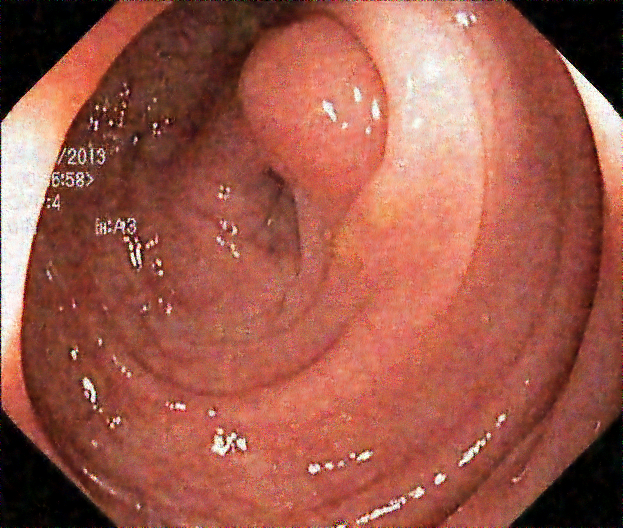
\includegraphics[width=\linewidth]{img/presentazione/dncnn/kvasir_denoise_dncnn_post_50.png}\\[0.3em]
            PSNR=26.4169
        \end{minipage} \\[1em]
        \begin{minipage}{0.28\linewidth}
            \centering
            \textbf{GT}\\[0.3em]
            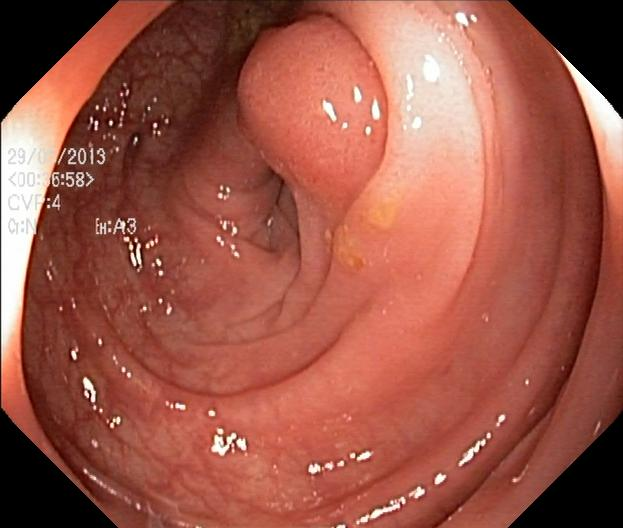
\includegraphics[width=\linewidth]{img/presentazione/kvasir.jpg}\\[0.3em]
            --
        \end{minipage} &
        \begin{minipage}{0.28\linewidth}
            \centering
            \textbf{Autoencoder}\\[0.3em]
            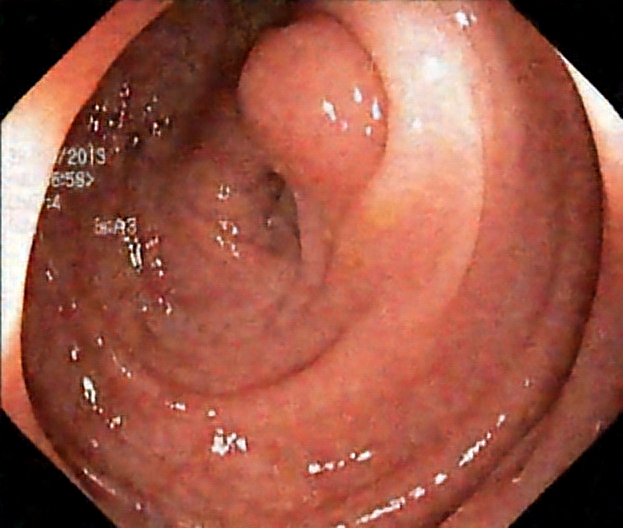
\includegraphics[width=\linewidth]{img/presentazione/autoen/kvasir_denoise_autoen_post_50.png}\\[0.3em]
            PSNR=28.7878
        \end{minipage} &
        \begin{minipage}{0.28\linewidth}
            % Cella vuota
        \end{minipage} \\
    \end{tabular}
\end{frame}







% far vedere meglio come funziona optuna
\begin{frame}{Studio degli iperparametri - 1}
  \begin{itemize}
    \item Studio di ottimizzazione degli iperparametri con Optuna.
    \item Ricerca automatica bayesiana ed evolutiva.
    \item Obiettivo: trovare configurazioni ottimali di learning rate, numero di filtri e profondità della rete.
    \item Massimizzazione di accuratezza e PSNR.
    \item Analisi sistematica per strategie di addestramento più robuste ed efficienti.
  \end{itemize}
\end{frame}
% optuna: strumento che serve a trovare iperparametri ottimali per il training con funzione obiettivo che minimizza la loss e massimizzare l'accuracy <- da dire nel discorso

% Slide 12: Studio iperparametri e fine tuning su RIDNet Student
\begin{frame}{Studio degli iperparametri - 2}
  \begin{itemize}
    \item Avendo appurato che la rete Ridnet è stata la migliore delle tre si è deciso di fare uno studio sui suoi iperparametri utilizzando il dataset di finetuning Kvasir
    \item Si sono ricercati valori migliori per riduzione e numero di feature map.
    \item \'E stato trovato feats=32 e reduction=8
    \item La nuova rete con i nuovi iperparametri è stata allenata sullo stesso dataset di training attraverso Distillazione Teacher-Student.
    \item Si nota un miglioramento del PSNR per soggetto della rete student rispetto alla rete teacher.
  \end{itemize}
\end{frame}

% --- Scheletro generico Denoising ---
% --- Confronto Denoising: Tamburo ---
% σ=15
% σ=15
\begin{frame}{Confronto Denoising: Tamburo ($\sigma=15$)}
    \centering
    \renewcommand{\arraystretch}{1.0} 
    \begin{tabular}{c c}
        % Prima riga
        \begin{minipage}{0.45\linewidth}
            \centering
            \textbf{Noisy}\\[0.1em]
            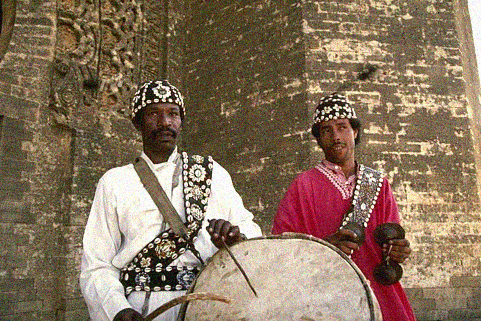
\includegraphics[width=0.8\linewidth]{img/presentazione/noisy/tamburo_noise_15.png}\\[0.1em]
            $\sigma=15$
        \end{minipage} &
        \begin{minipage}{0.45\linewidth}
            \centering
            \textbf{RidNet Teacher}\\[0.1em]
            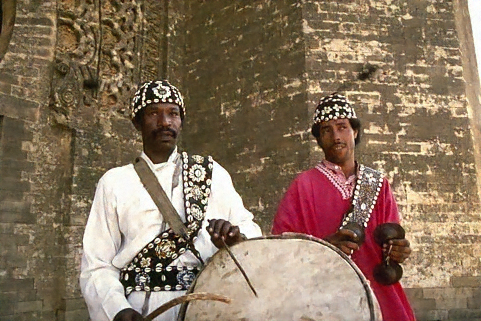
\includegraphics[width=0.8\linewidth]{img/presentazione/ridnet/tamburo_denoise_ridnet_15.png}\\[0.1em]
            PSNR=30.4905
        \end{minipage} \\[0.4em]
        % Seconda riga
        \begin{minipage}{0.45\linewidth}
            \centering
            \textbf{GT}\\[0.1em]
            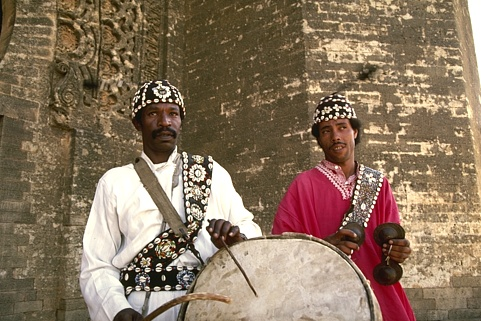
\includegraphics[width=0.8\linewidth]{img/presentazione/bsd_tamburo.jpg}\\[0.1em]
            --
        \end{minipage} &
        \begin{minipage}{0.45\linewidth}
            \centering
            \textbf{RidNet Student}\\[0.1em]
            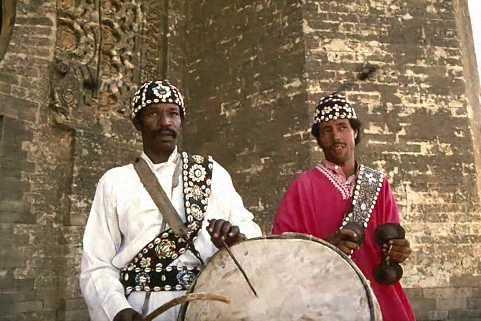
\includegraphics[width=0.8\linewidth]{img/presentazione/ridnetstudent/tamburo_denoise_ridnetstudent_15.png}\\[0.1em]
            PSNR=30.5752
        \end{minipage} \\
    \end{tabular}
\end{frame}

% σ=25
\begin{frame}{Confronto Denoising: Tamburo ($\sigma=25$)}
    \centering
    \renewcommand{\arraystretch}{1.0}
    \begin{tabular}{c c}
        \begin{minipage}{0.45\linewidth}
            \centering
            \textbf{Noisy}\\[0.1em]
            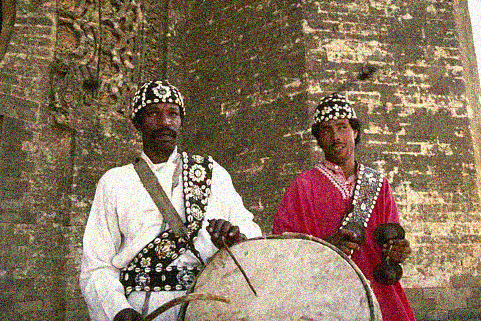
\includegraphics[width=0.8\linewidth]{img/presentazione/noisy/tamburo_noise_25.png}\\[0.1em]
            $\sigma=25$
        \end{minipage} &
        \begin{minipage}{0.45\linewidth}
            \centering
            \textbf{RidNet Teacher}\\[0.1em]
            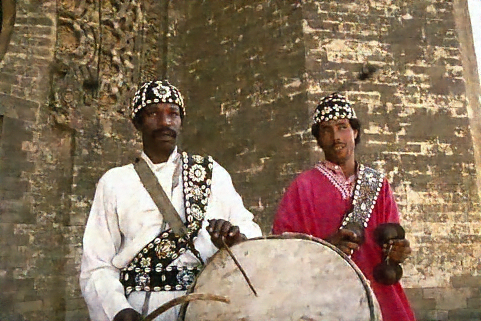
\includegraphics[width=0.8\linewidth]{img/presentazione/ridnet/tamburo_denoise_ridnet_25.png}\\[0.1em]
            PSNR=27.7076
        \end{minipage} \\[0.4em]
        \begin{minipage}{0.45\linewidth}
            \centering
            \textbf{GT}\\[0.1em]
            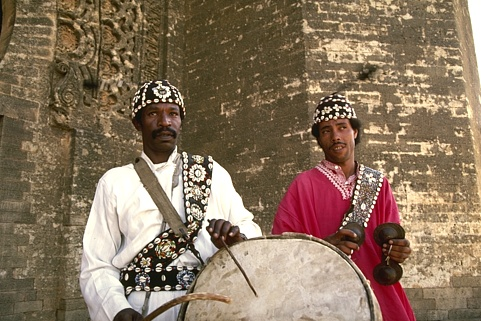
\includegraphics[width=0.8\linewidth]{img/presentazione/bsd_tamburo.jpg}\\[0.1em]
            --
        \end{minipage} &
        \begin{minipage}{0.45\linewidth}
            \centering
            \textbf{RidNet Student}\\[0.1em]
            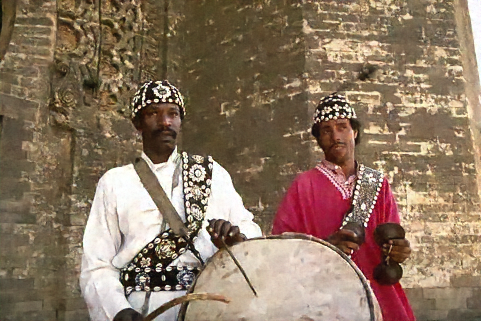
\includegraphics[width=0.8\linewidth]{img/presentazione/ridnetstudent/tamburo_denoise_ridnetstudent_25.png}\\[0.1em]
            PSNR=27.7244
        \end{minipage} \\
    \end{tabular}
\end{frame}

% σ=50
\begin{frame}{Confronto Denoising: Tamburo ($\sigma=50$)}
    \centering
    \renewcommand{\arraystretch}{1.0}
    \begin{tabular}{c c}
        \begin{minipage}{0.45\linewidth}
            \centering
            \textbf{Noisy}\\[0.1em]
            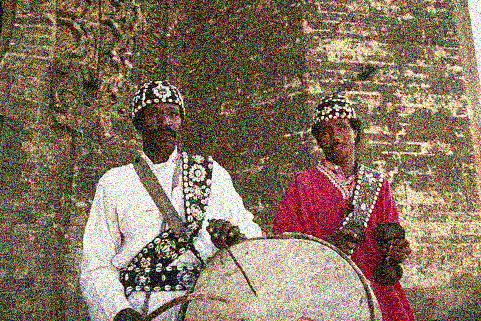
\includegraphics[width=0.8\linewidth]{img/presentazione/noisy/tamburo_noise_50.png}\\[0.1em]
            $\sigma=50$
        \end{minipage} &
        \begin{minipage}{0.45\linewidth}
            \centering
            \textbf{RidNet Teacher}\\[0.1em]
            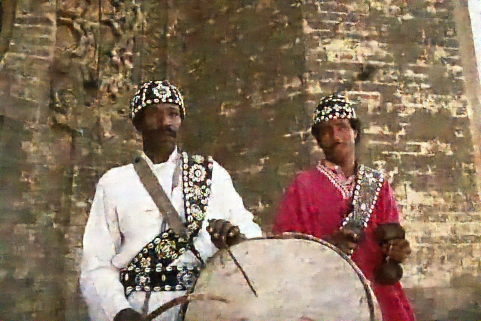
\includegraphics[width=0.8\linewidth]{img/presentazione/ridnet/tamburo_denoise_ridnet_50.png}\\[0.1em]
            PSNR=24.2318
        \end{minipage} \\[0.4em]
        \begin{minipage}{0.45\linewidth}
            \centering
            \textbf{GT}\\[0.1em]
            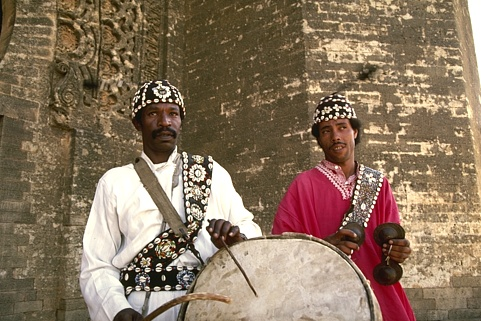
\includegraphics[width=0.8\linewidth]{img/presentazione/bsd_tamburo.jpg}\\[0.1em]
            --
        \end{minipage} &
        \begin{minipage}{0.45\linewidth}
            \centering
            \textbf{RidNet Student}\\[0.1em]
            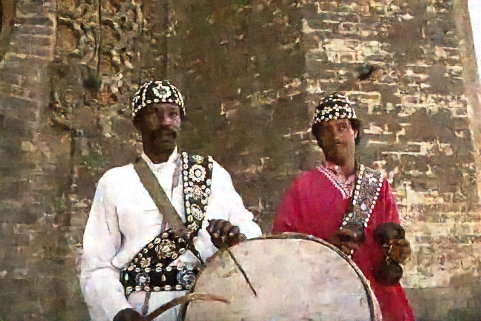
\includegraphics[width=0.8\linewidth]{img/presentazione/ridnetstudent/tamburo_denoise_ridnetstudent_50.png}\\[0.1em]
            PSNR=24.4879
        \end{minipage} \\
    \end{tabular}
\end{frame}

\begin{frame}{Confronto Denoising: Scacchi ($\sigma \approx 16.47$)}
    \centering
    \renewcommand{\arraystretch}{1.0}
    \begin{tabular}{c c}
        % Prima riga
        \begin{minipage}{0.4\linewidth}
            \centering
            \textbf{Noisy}\\[0.1em]
            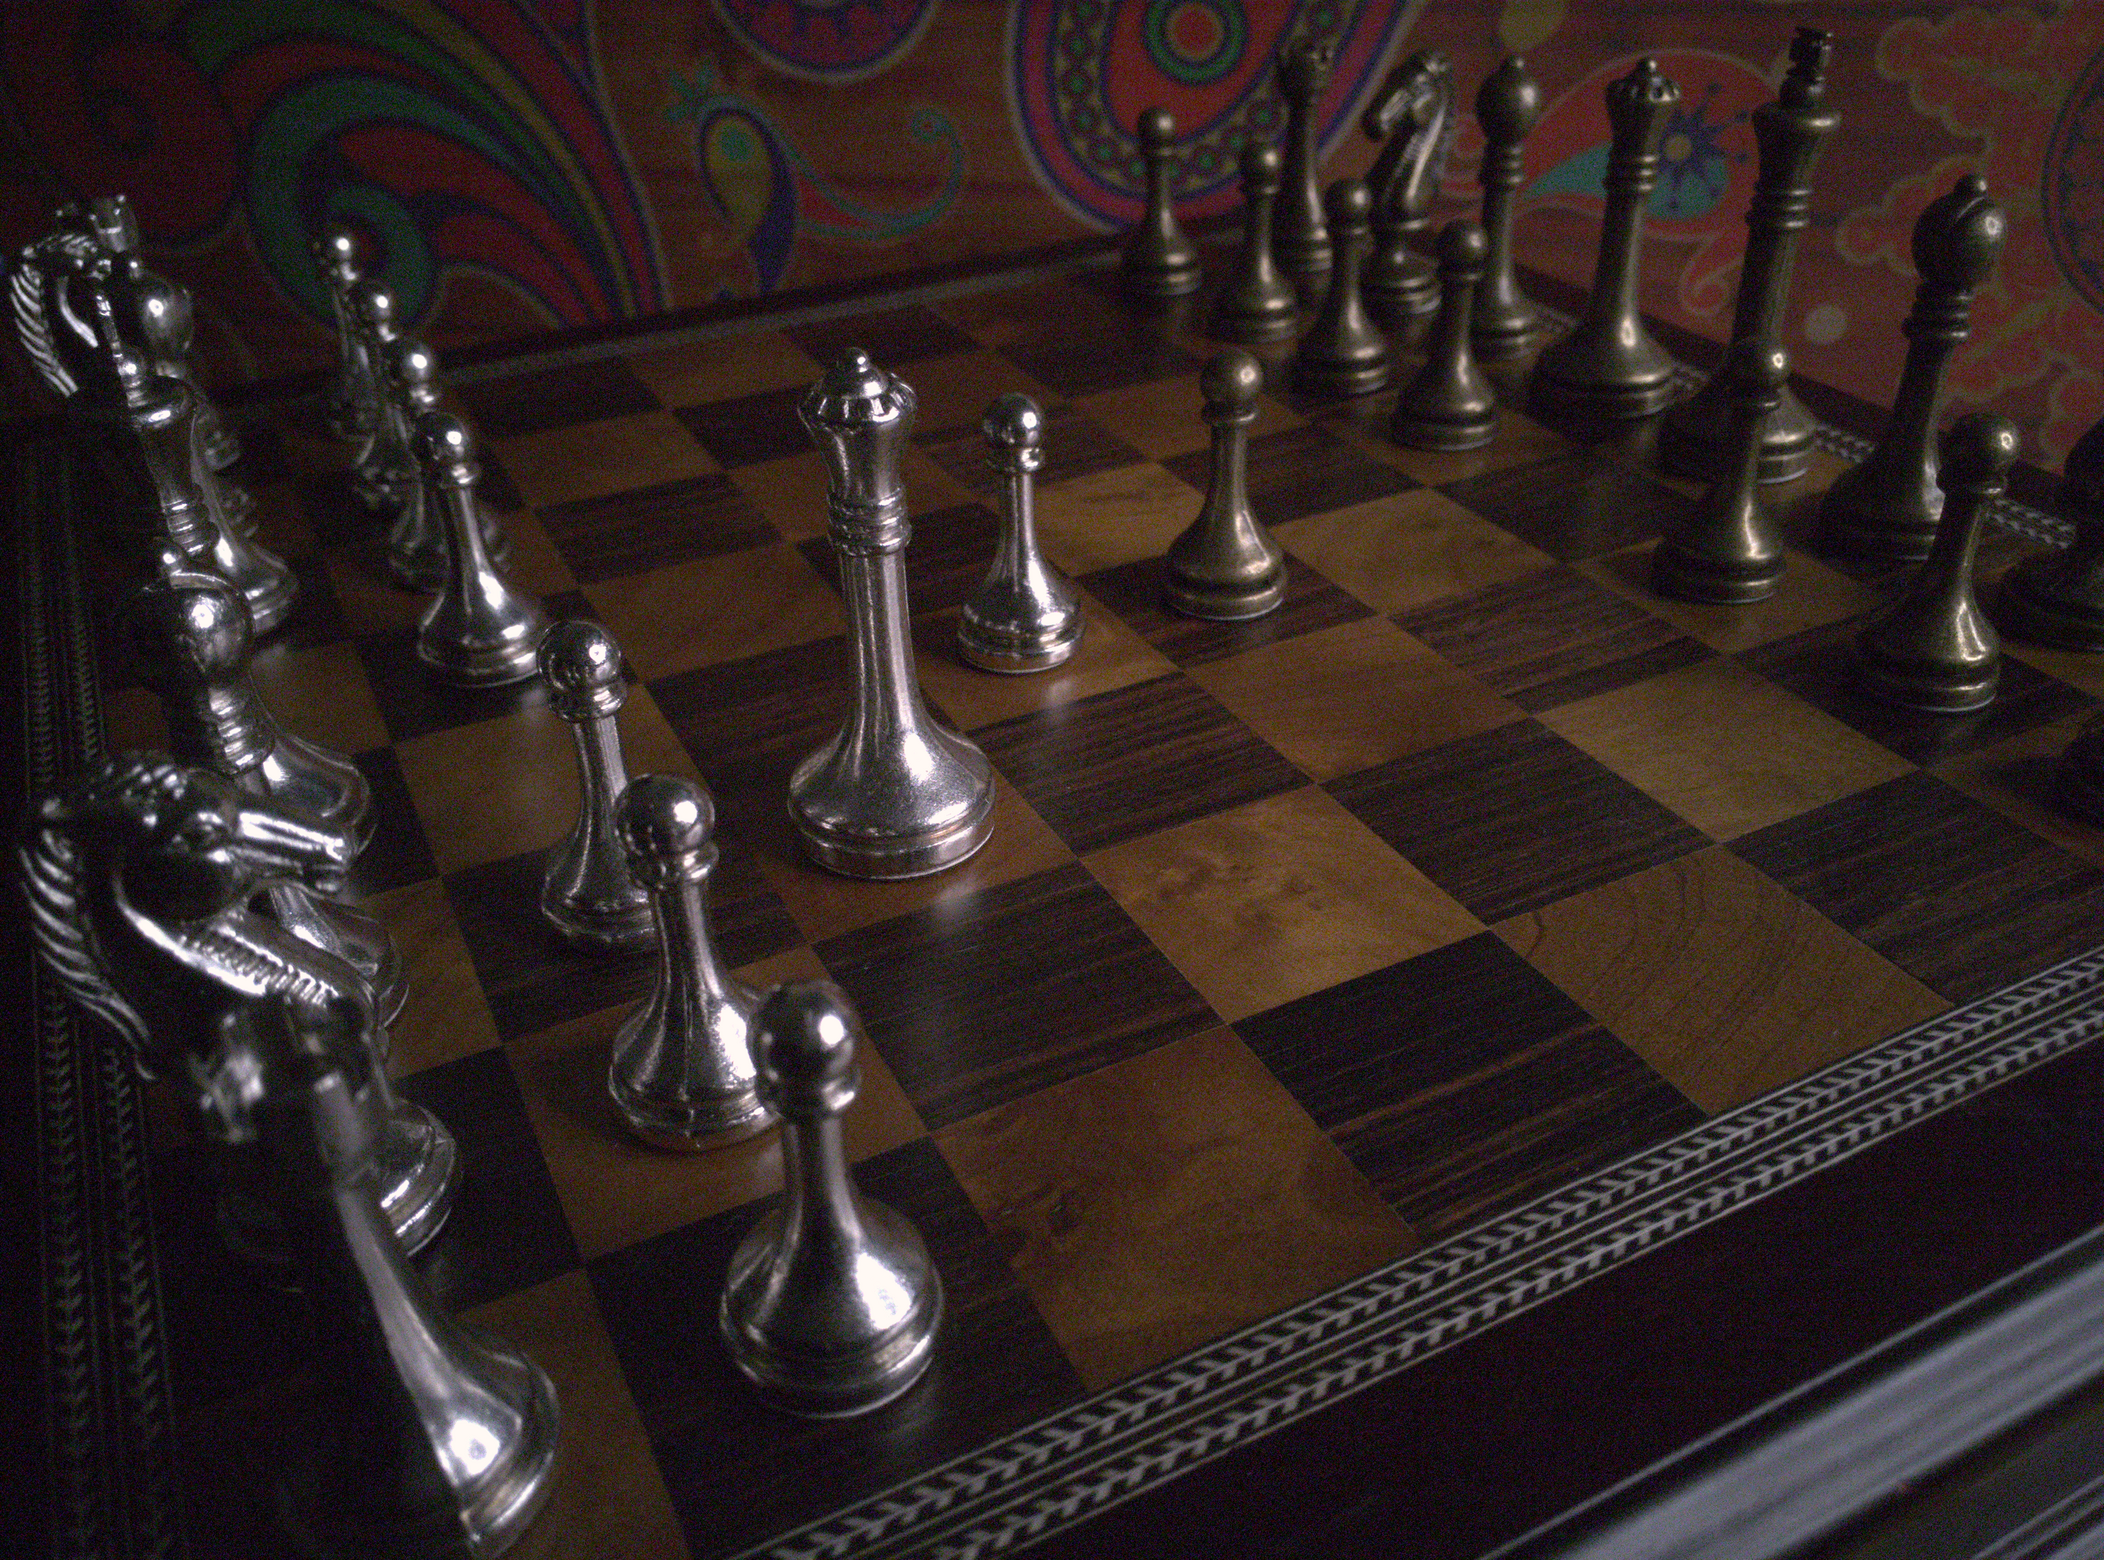
\includegraphics[height=0.3\textheight]{img/presentazione/sidd_scacchi_noise.PNG}\\[0.1em]
            $\sigma \approx 16.47$
        \end{minipage} &
        \begin{minipage}{0.4\linewidth}
            \centering
            \textbf{RidNet Teacher}\\[0.1em]
            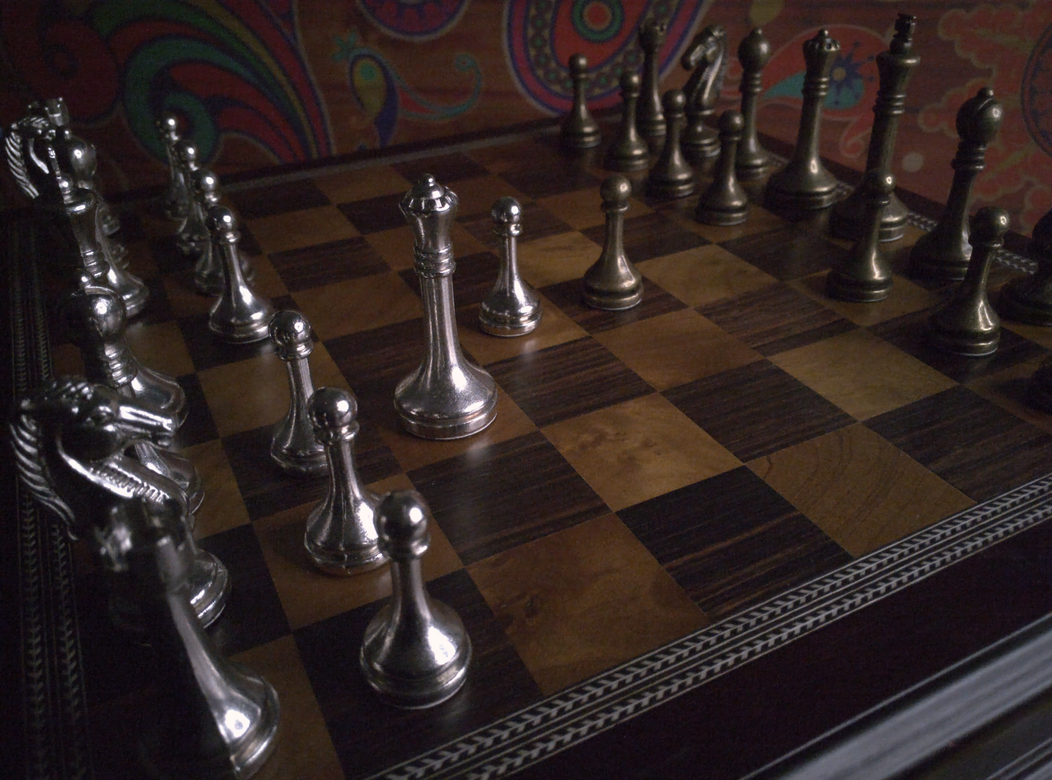
\includegraphics[height=0.3\textheight]{img/presentazione/ridnet/scacchi_denoise_ridnet.png}\\[0.1em]
            PSNR=34.4284
        \end{minipage} \\[0.4em]
        % Seconda riga
        \begin{minipage}{0.4\linewidth}
            \centering
            \textbf{GT}\\[0.1em]
            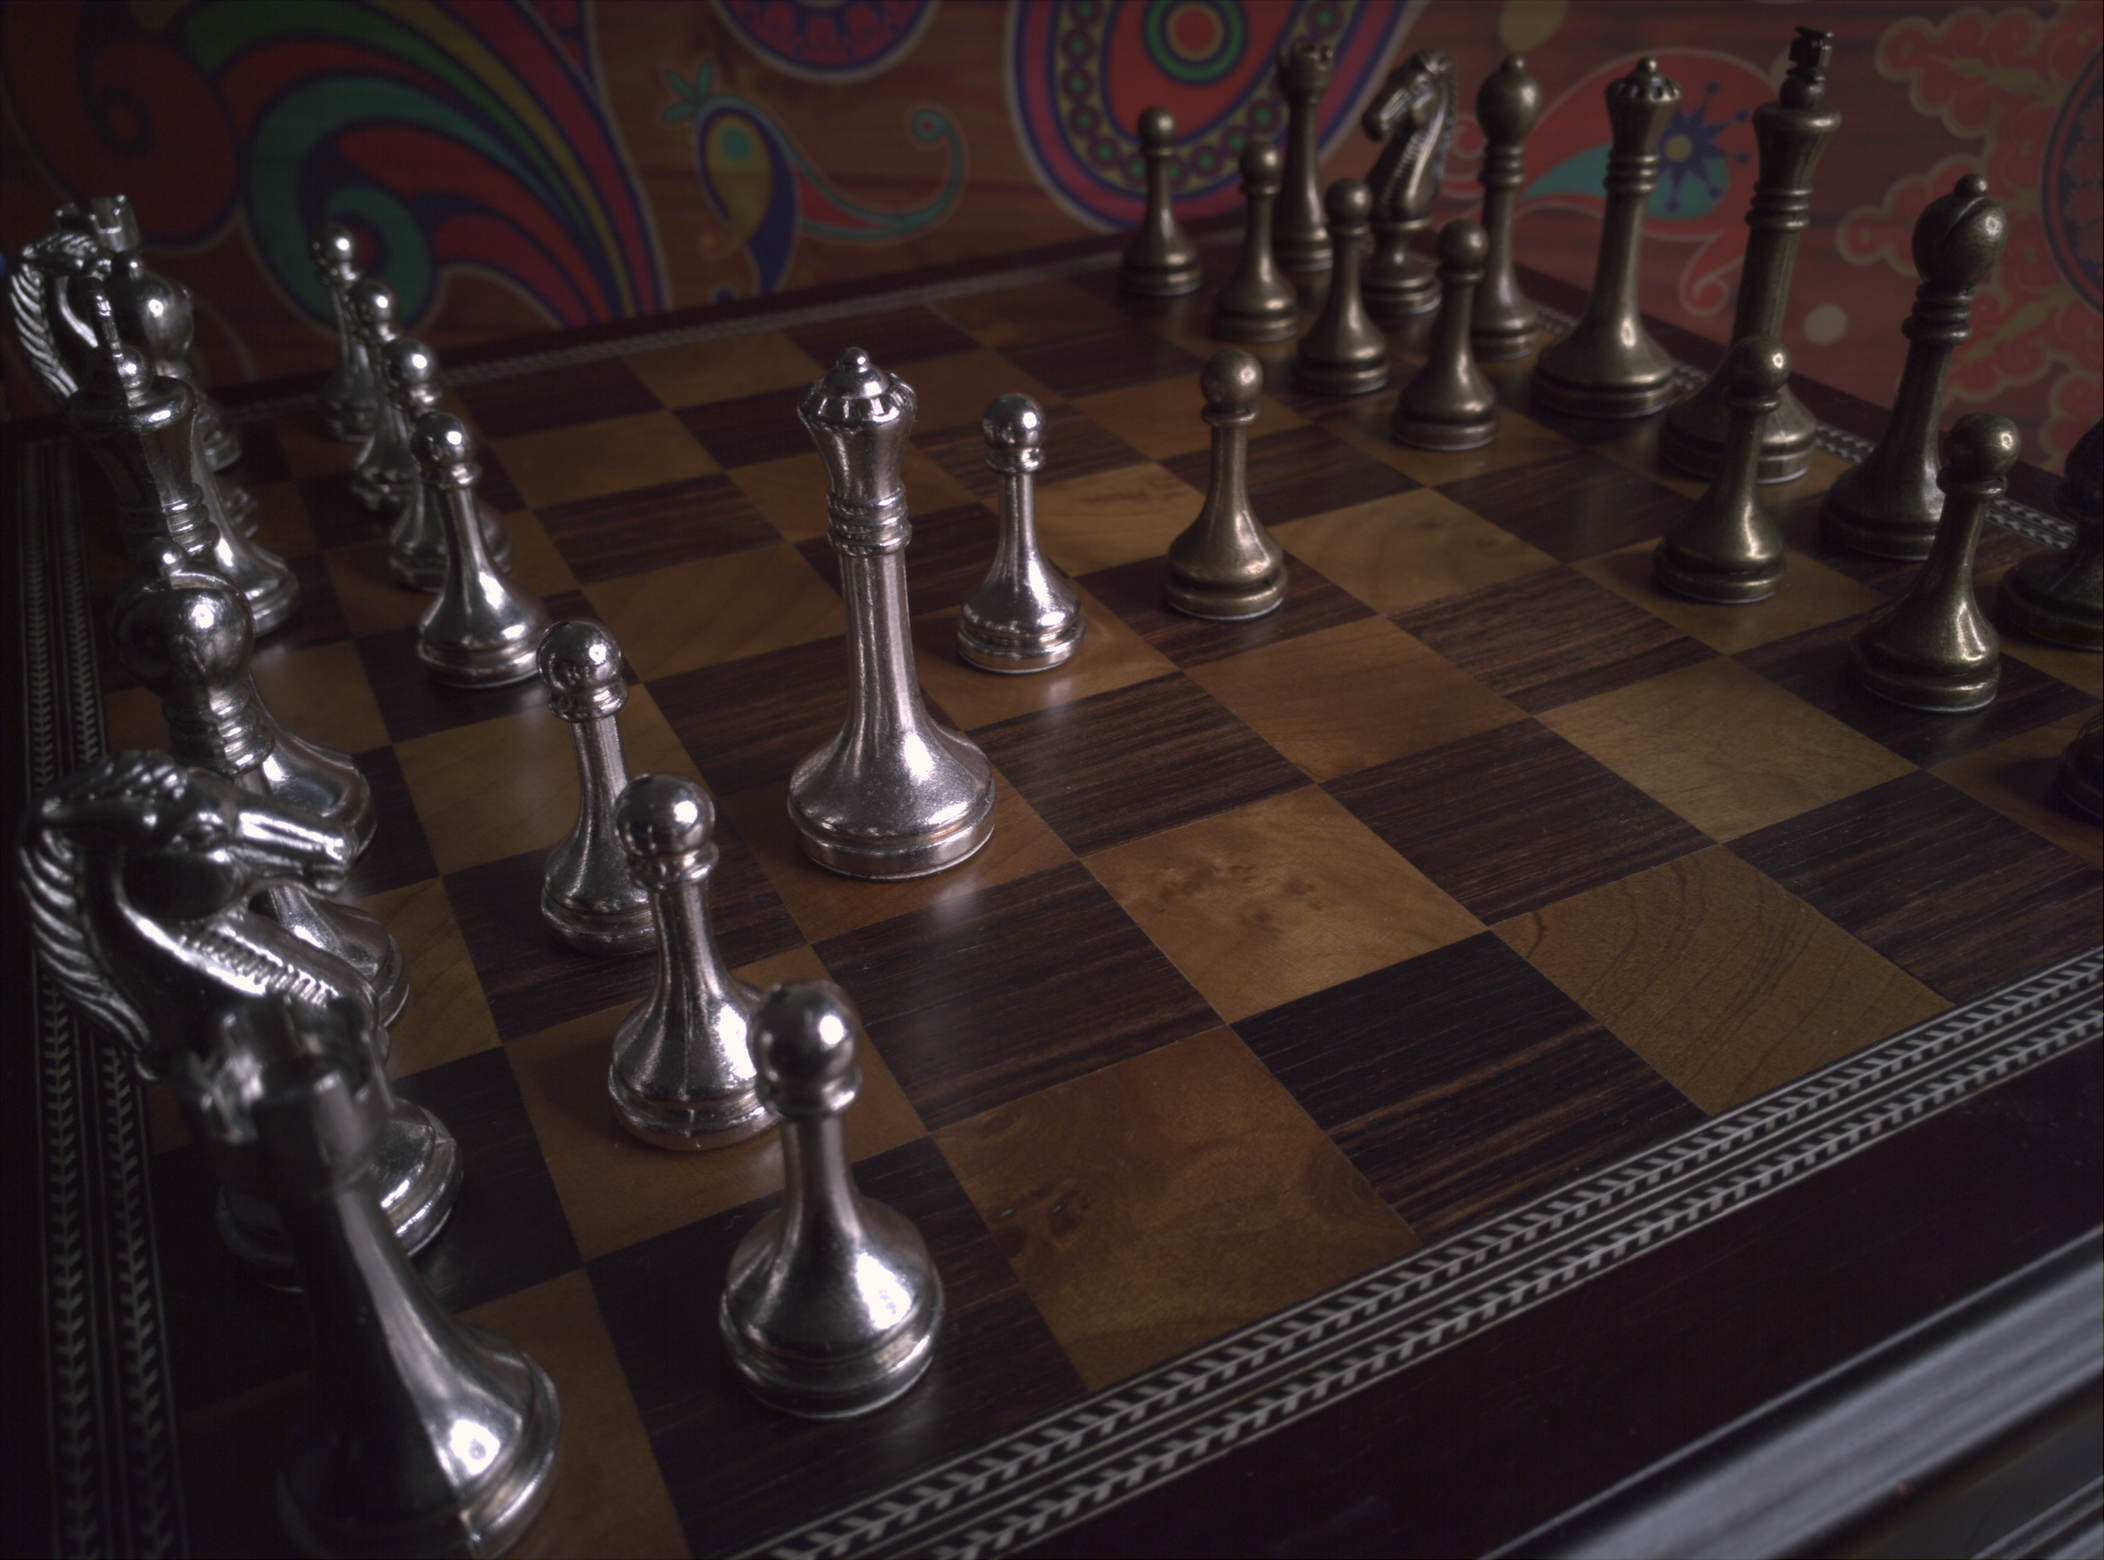
\includegraphics[height=0.3\textheight]{img/presentazione/sidd_scacchi_gt.PNG}\\[0.1em]
            --
        \end{minipage} &
        \begin{minipage}{0.4\linewidth}
            \centering
            \textbf{RidNet Student}\\[0.1em]
            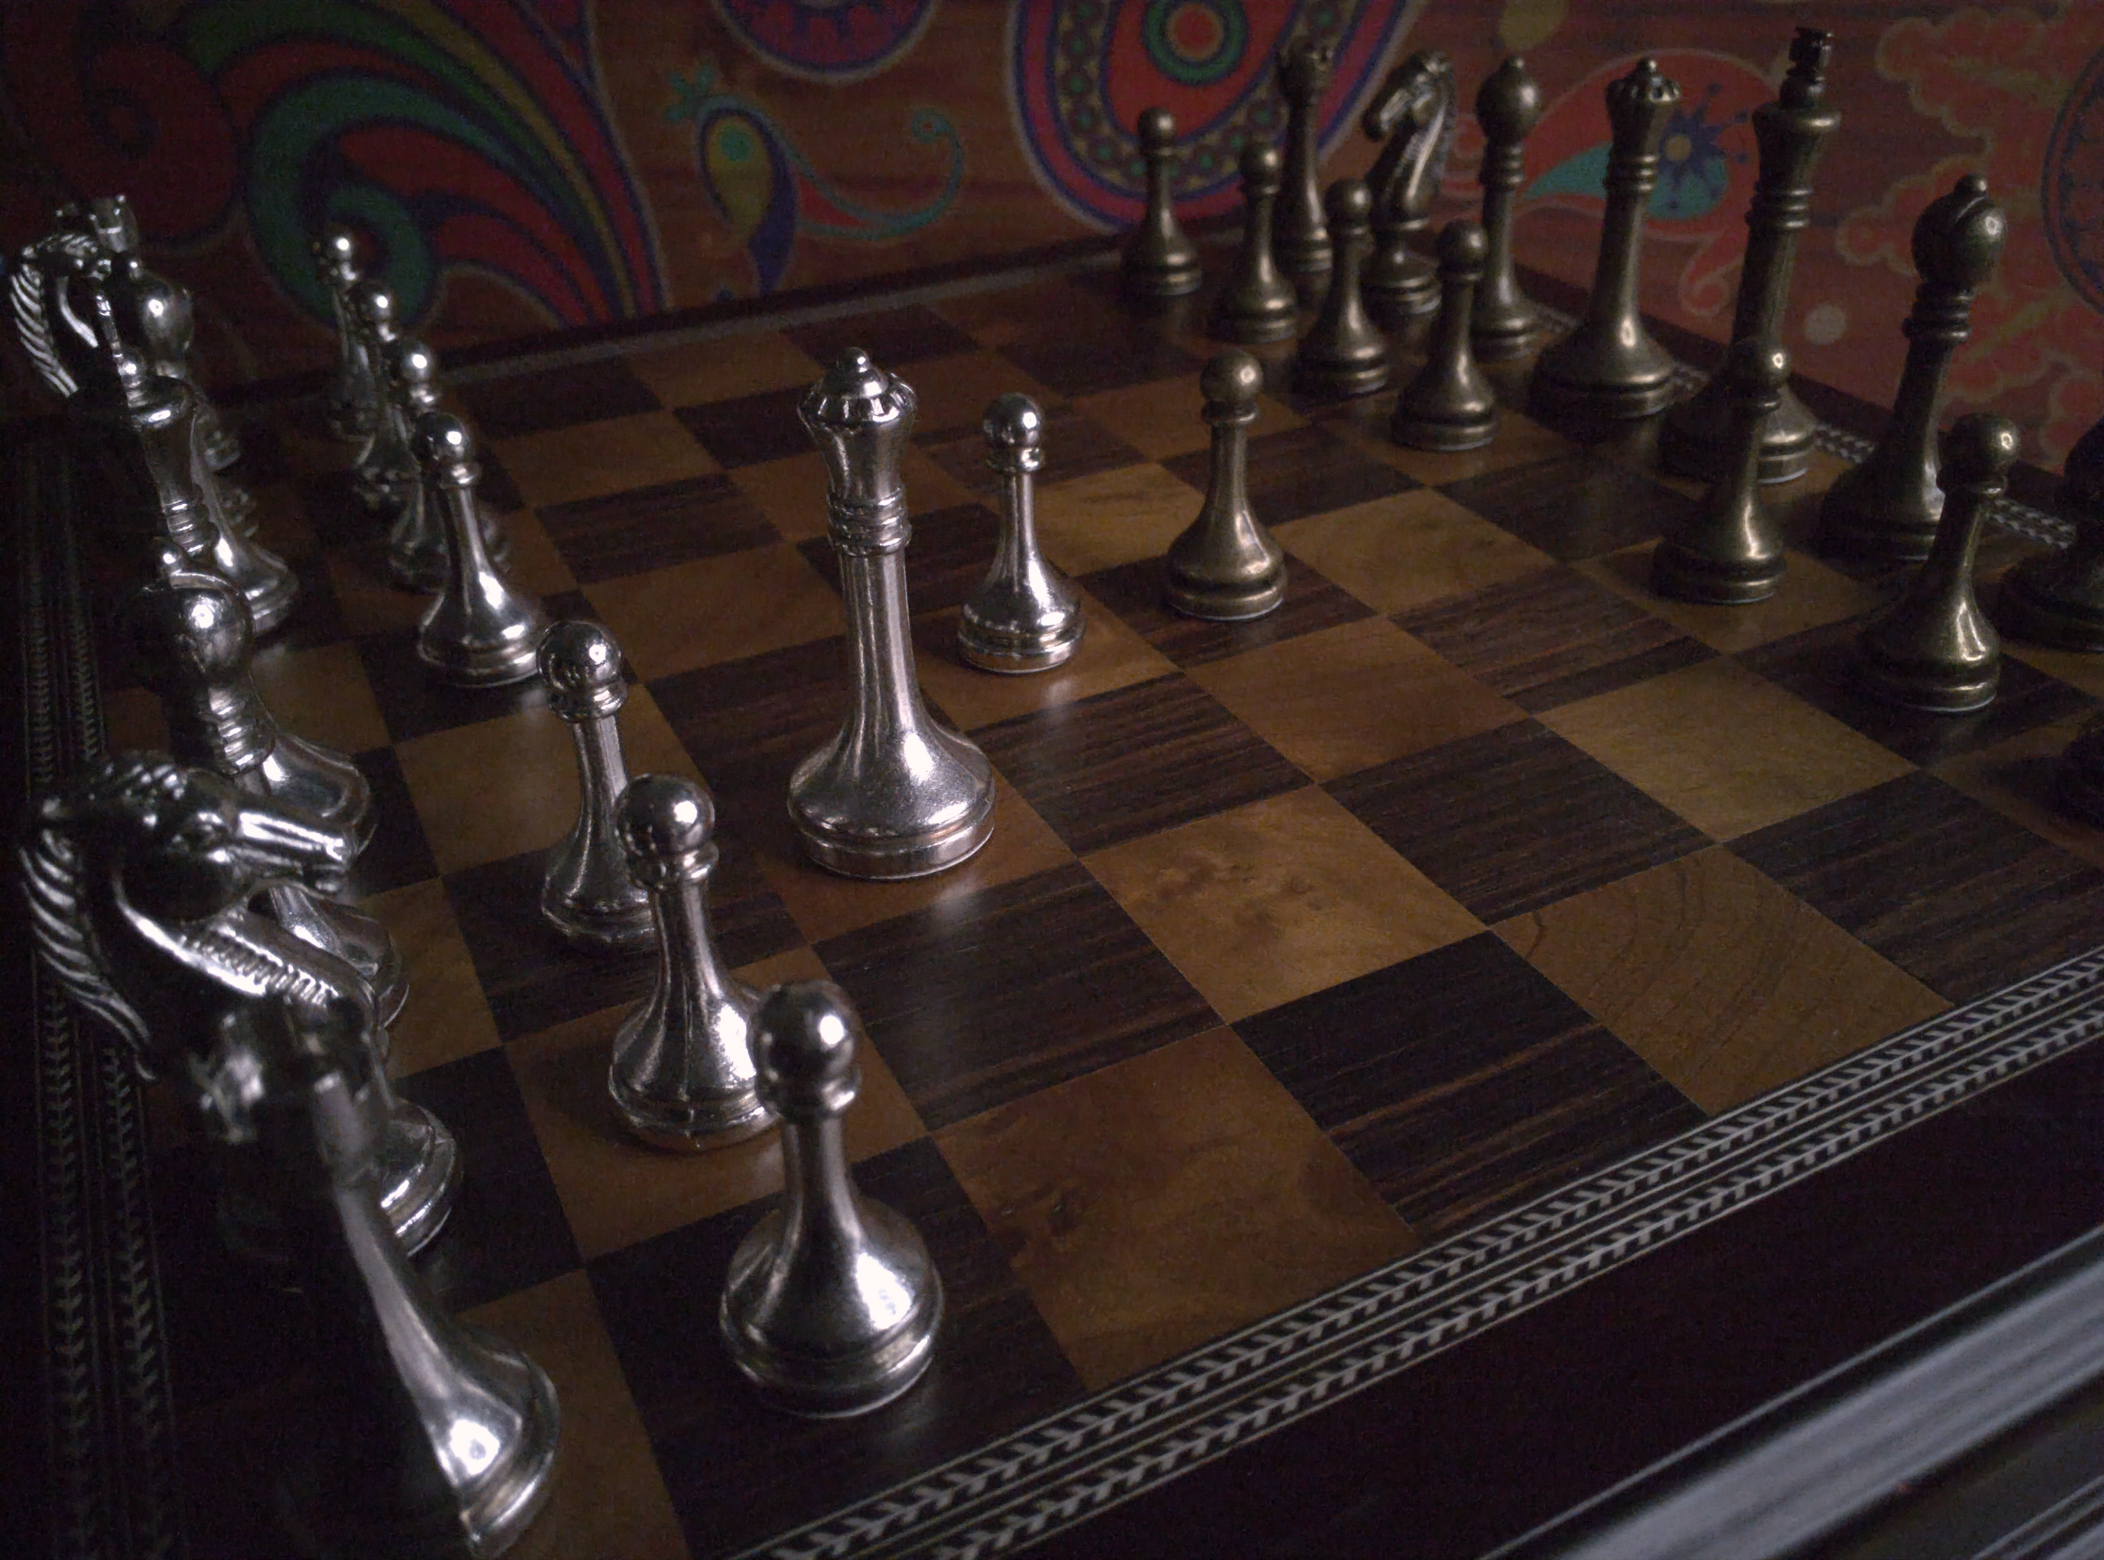
\includegraphics[height=0.3\textheight]{img/presentazione/ridnetstudent/scacchi_denoise_ridnetstudent.png}\\[0.1em]
            PSNR=35.8899
        \end{minipage} \\
    \end{tabular}
\end{frame}




\begin{frame}{Fine Tuning su RIDNet Student}
  \begin{itemize}
    \item Il modello RIDNet Student è stato sottoposto a fine tuning.
    \item I risultati finali evidenziano un incremento del PSNR e della qualità visiva rispetto alla versione pre-addestrata e al Teacher post Fine Tuning, confermando l'efficacia degli iperparametri trovati.
  \end{itemize}
\end{frame}


% --- Fine tuning σ=15 ---
\begin{frame}{Fine Tuning Student $\sigma=15$}
    \centering
    \renewcommand{\arraystretch}{1.5}
    \begin{tabular}{c c c}
        \begin{minipage}{0.28\linewidth}
            \centering
            \small{\textbf{Noisy}}\\[0.3em]
            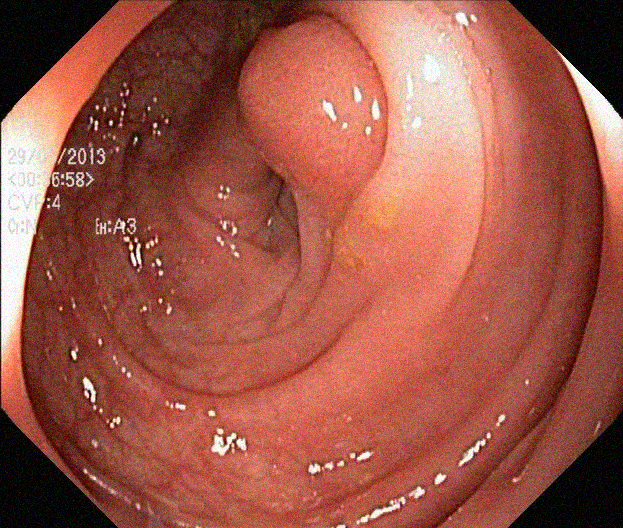
\includegraphics[width=\linewidth]{img/presentazione/noisy/kvasir_noise_15.png}\\[0.3em]
            $\sigma=15$
        \end{minipage} &
        \begin{minipage}{0.28\linewidth}
            \centering
            \small{\textbf{RidNet Teacher pre}}\\[0.3em]
            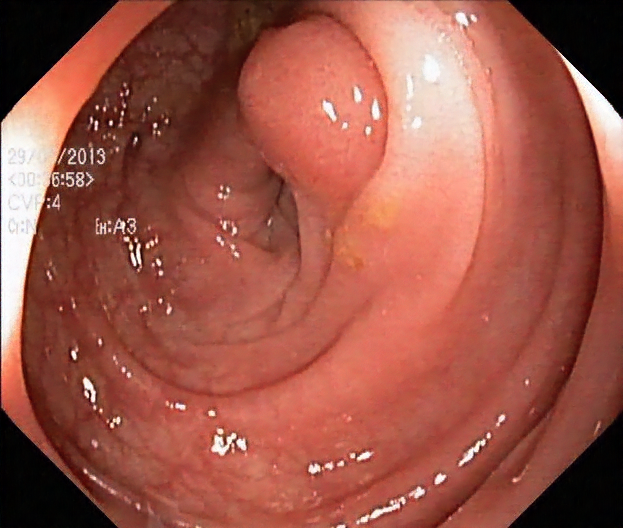
\includegraphics[width=\linewidth]{img/presentazione/ridnet/kvasir_denoise_ridnet_pre_15.png}\\[0.3em]
            PSNR=35.3678
        \end{minipage} &
        \begin{minipage}{0.28\linewidth}
            \centering
            \small{\textbf{RidNet Student pre}}\\[0.3em]
            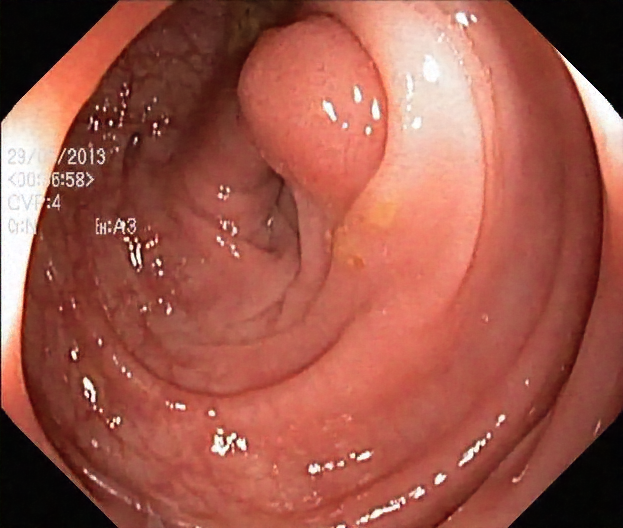
\includegraphics[width=\linewidth]{img/presentazione/ridnetstudent/kvasir_denoise_ridnetstudent_pre_15.png}\\[0.3em]
            PSNR=34.8715
        \end{minipage} \\[1em]
        \begin{minipage}{0.28\linewidth}
            \centering
            \textbf{GT}\\[0.3em]
            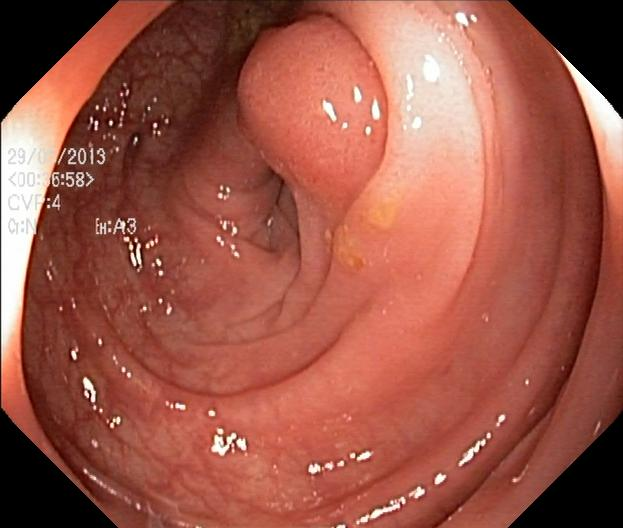
\includegraphics[width=\linewidth]{img/presentazione/kvasir.jpg}\\[0.3em]
            --
        \end{minipage} &
        \begin{minipage}{0.28\linewidth}
            \centering
            \small{\textbf{RidNet Teacher post}}\\[0.3em]
            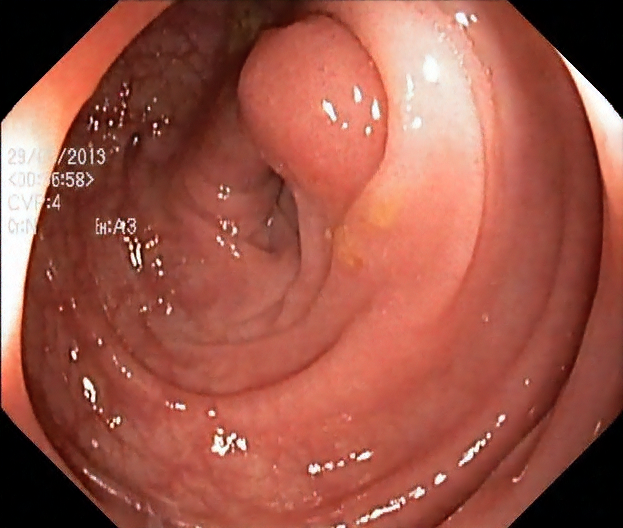
\includegraphics[width=\linewidth]{img/presentazione/ridnet/kvasir_denoise_ridnet_post_15.png}\\[0.3em]
            PSNR=35.7874
        \end{minipage} &
        \begin{minipage}{0.28\linewidth}
            \centering
            \small{\textbf{RidNet Student post}}\\[0.3em]
            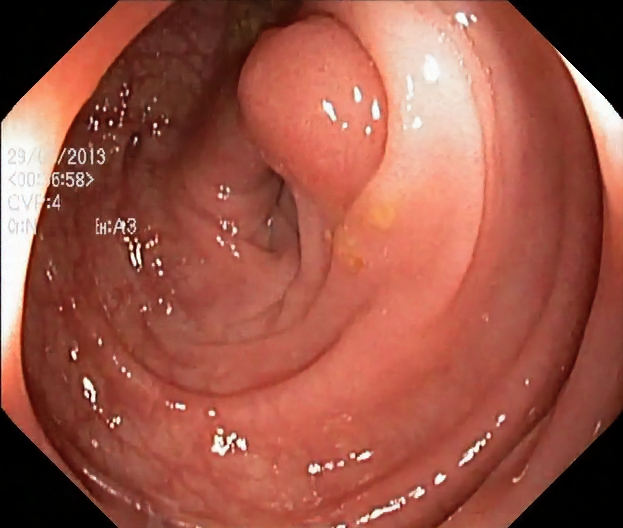
\includegraphics[width=\linewidth]{img/presentazione/ridnetstudent/kvasir_denoise_ridnetstudent_post_15.png}\\[0.3em]
            PSNR=36.4744
        \end{minipage}  \\
    \end{tabular}
\end{frame}

% --- Fine tuning σ=25 ---
\begin{frame}{Fine Tuning Student $\sigma=25$}
    \centering
    \renewcommand{\arraystretch}{1.5}
    \begin{tabular}{c c c}
        \begin{minipage}{0.28\linewidth}
            \centering
            \small{\textbf{Noisy}}\\[0.3em]
            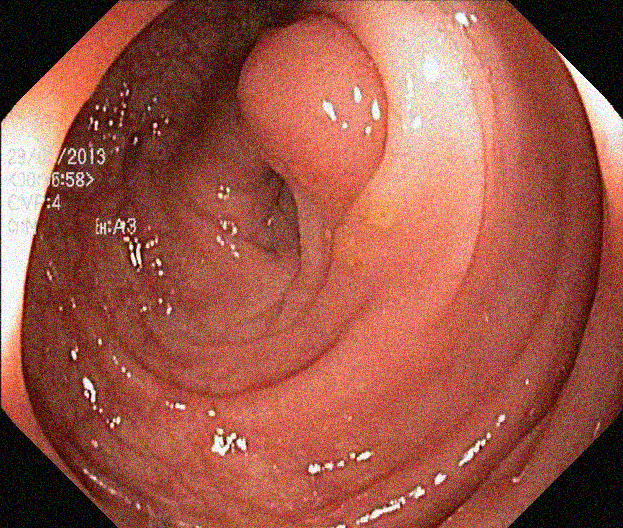
\includegraphics[width=\linewidth]{img/presentazione/noisy/kvasir_noise_25.png}\\[0.3em]
            $\sigma=25$
        \end{minipage} &
        \begin{minipage}{0.28\linewidth}
            \centering
            \small{\textbf{RidNet Teacher pre}}\\[0.3em]
            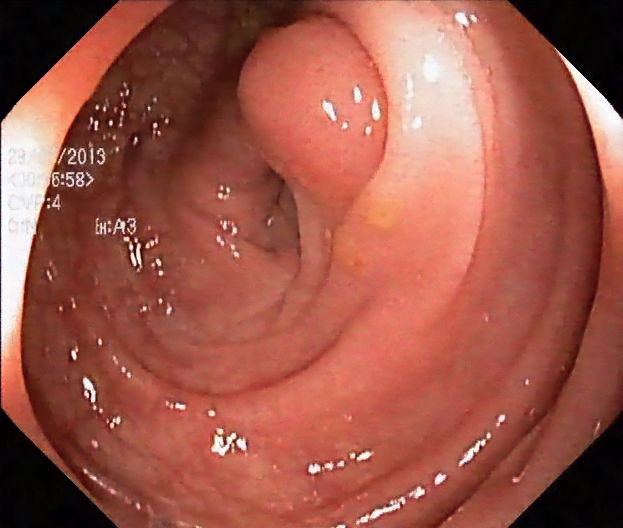
\includegraphics[width=\linewidth]{img/presentazione/ridnet/kvasir_denoise_ridnet_pre_25.png}\\[0.3em]
            PSNR=32.9191
        \end{minipage} &
        \begin{minipage}{0.28\linewidth}
            \centering
            \small{\textbf{RidNet Student pre}}\\[0.3em]
            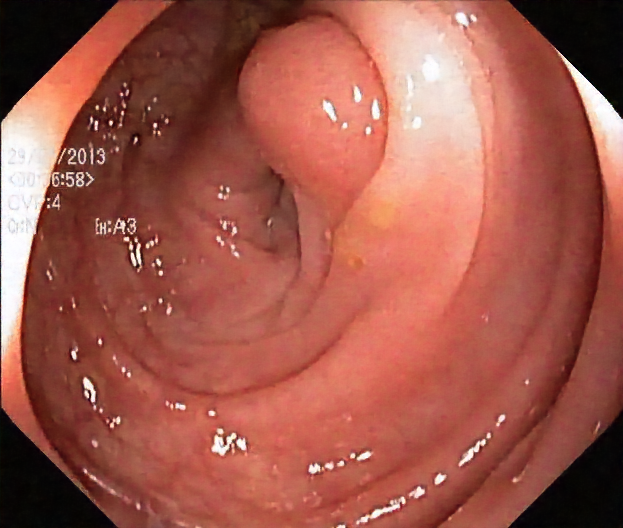
\includegraphics[width=\linewidth]{img/presentazione/ridnetstudent/kvasir_denoise_ridnetstudent_pre_25.png}\\[0.3em]
            PSNR=32.2314
        \end{minipage} \\[1em]
        \begin{minipage}{0.28\linewidth}
            \centering
            \textbf{GT}\\[0.3em]
            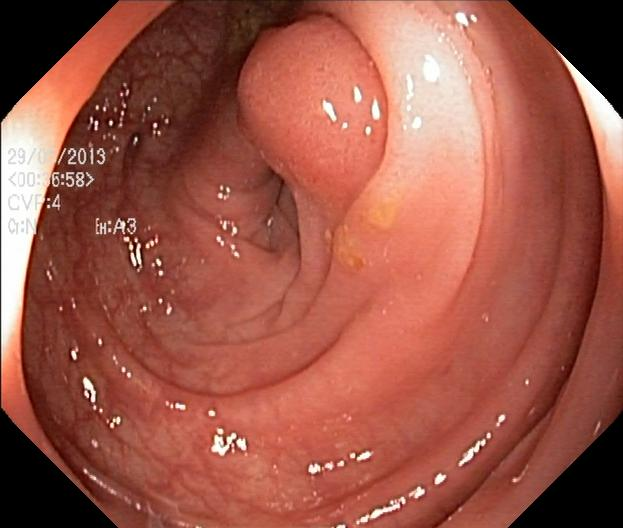
\includegraphics[width=\linewidth]{img/presentazione/kvasir.jpg}\\[0.3em]
            --
        \end{minipage} &
        \begin{minipage}{0.28\linewidth}
            \centering
            \small{\textbf{RidNet Teacher post}}\\[0.3em]
            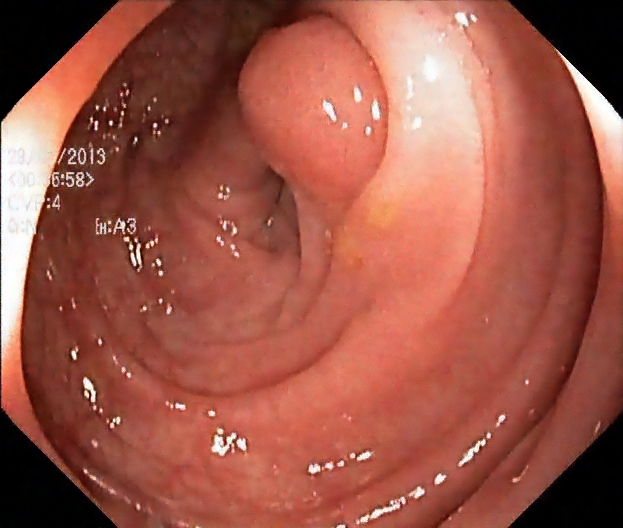
\includegraphics[width=\linewidth]{img/presentazione/ridnet/kvasir_denoise_ridnet_post_25.png}\\[0.3em]
            PSNR=33.4563
        \end{minipage} &
        \begin{minipage}{0.28\linewidth}
            \centering
            \small{\textbf{RidNet Student post}}\\[0.3em]
            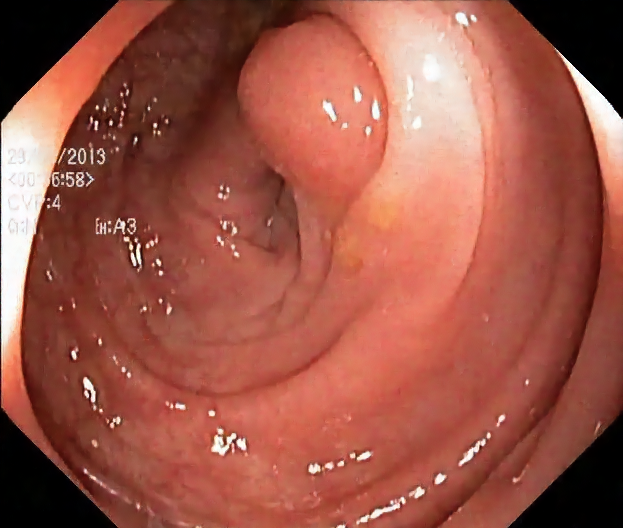
\includegraphics[width=\linewidth]{img/presentazione/ridnetstudent/kvasir_denoise_ridnetstudent_post_25.png}\\[0.3em]
            PSNR=34.1592
        \end{minipage}  \\
    \end{tabular}
\end{frame}

% --- Fine tuning σ=50 ---
\begin{frame}{Fine Tuning Student $\sigma=50$}
    \centering
    \renewcommand{\arraystretch}{1.5}
    \begin{tabular}{c c c}
        \begin{minipage}{0.28\linewidth}
            \centering
            \small{\textbf{Noisy}}\\[0.3em]
            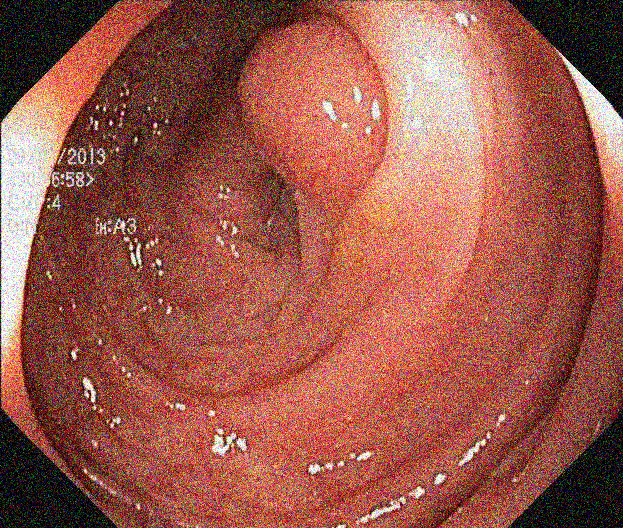
\includegraphics[width=\linewidth]{img/presentazione/noisy/kvasir_noise_50.png}\\[0.3em]
            $\sigma=50$
        \end{minipage} &
        \begin{minipage}{0.28\linewidth}
            \centering
            \small{\textbf{RidNet Teacher pre}}\\[0.3em]
            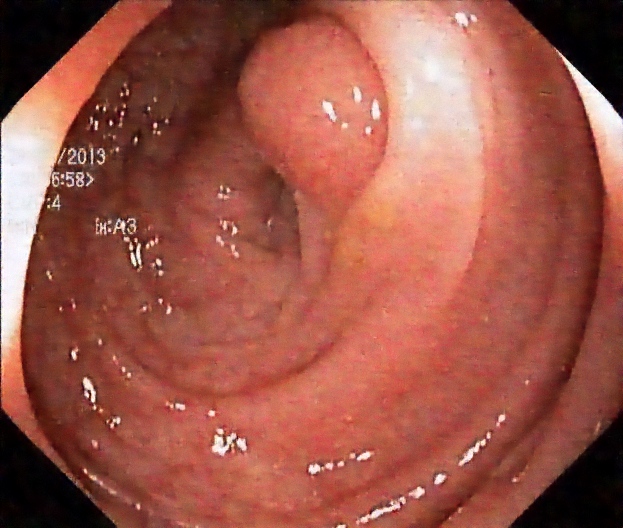
\includegraphics[width=\linewidth]{img/presentazione/ridnet/kvasir_denoise_ridnet_pre_50.png}\\[0.3em]
            PSNR=29.4796
        \end{minipage} &
        \begin{minipage}{0.28\linewidth}
            \centering
            \small{\textbf{RidNet Student pre}}\\[0.3em]
            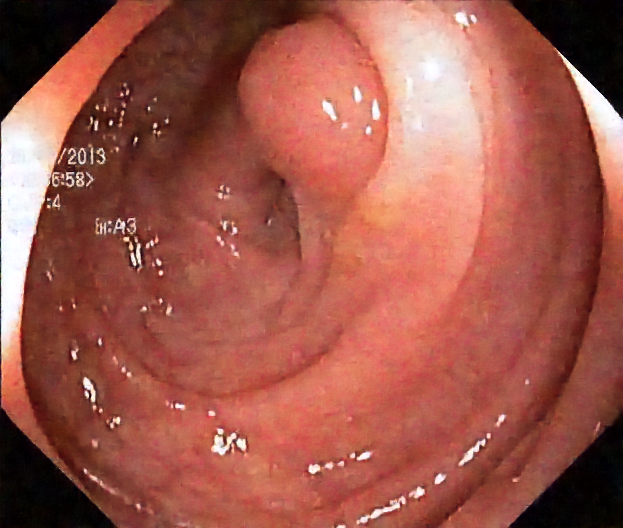
\includegraphics[width=\linewidth]{img/presentazione/ridnetstudent/kvasir_denoise_ridnetstudent_pre_50.png}\\[0.3em]
            PSNR=29.8349
        \end{minipage} \\[1em]
        \begin{minipage}{0.28\linewidth}
            \centering
            \textbf{GT}\\[0.3em]
            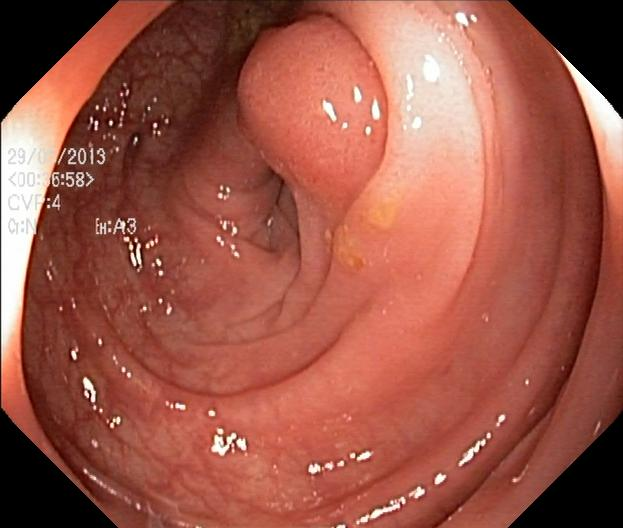
\includegraphics[width=\linewidth]{img/presentazione/kvasir.jpg}\\[0.3em]
            --
        \end{minipage} &
        \begin{minipage}{0.28\linewidth}
            \centering
            \small{\textbf{RidNet Teacher post}}\\[0.3em]
            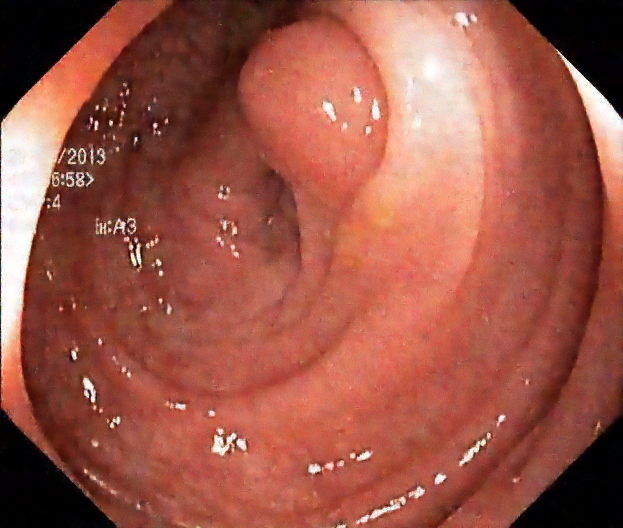
\includegraphics[width=\linewidth]{img/presentazione/ridnet/kvasir_denoise_ridnet_post_50.png}\\[0.3em]
            PSNR=29.8183
        \end{minipage} &
        \begin{minipage}{0.28\linewidth}
            \centering
            \small{\textbf{RidNet Student post}}\\[0.3em]
            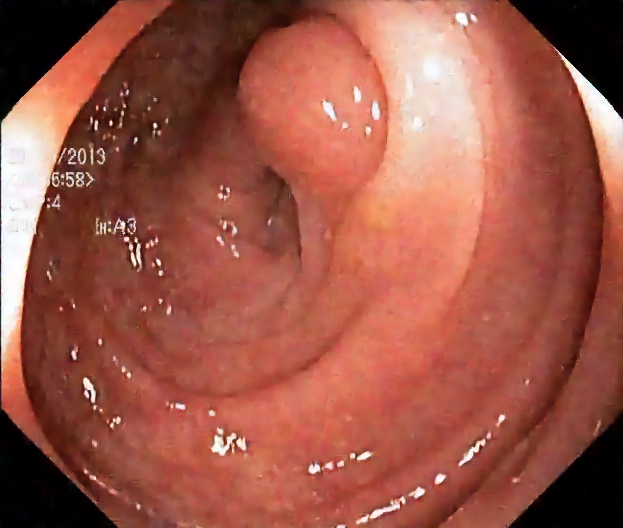
\includegraphics[width=\linewidth]{img/presentazione/ridnetstudent/kvasir_denoise_ridnetstudent_post_50.png}\\[0.3em]
            PSNR=30.9769
        \end{minipage}  \\
    \end{tabular}
\end{frame}







% Slide 13: Conclusioni
\begin{frame}{Conclusioni}
    \begin{itemize}
        \item Il denoising è un problema centrale nell'elaborazione delle immagini
        \item Le reti moderne offrono risultati superiori ai metodi classici
        \item La scelta del modello dipende dal contesto e dal tipo di rumore
    \end{itemize}
\end{frame}

\begin{frame}
    \centering
    \Huge{Grazie per l'attenzione!}
\end{frame}


\end{document}
